\chapter{Simulation}
Two levels are discussed in this section. First the simulation of single time series.
This is necessary to investigate the power of particle filters in 
identifying the BOLD model in a noisy environment. If the particle filter is unable
to get back to the "true" time-series in spite of noise then the particle filter
will not be useful. Additionally, determination of reasonable parameters from the
time-series is also desirable. The second simulation technique will be on a 
large group of voxels. Although the current technique treats each voxel separately,
the "Possum" FMRI simulation tool models noise more realistically, and provides additional
incite into the applicability of particle filters in modeling the BOLD signal on a large
scale.

\section{Single Timeseries}
Given the state-space equations for the BOLD signal, simulating a single time 
series is relatively straight forward. After a "true" signal is generated,
I then add identically and independently distributed (I.I.D.) Gaussian noise and a Wiener
process with Gaussian, I.I.D. steps. Finally a "carrier level" is added, since BOLD is typically
measured as a \% difference from the baseline. Although technically the particle filter
algorithm will immediately remove this, and calculate the \% difference, adding a carrier 
level means that the exact same algorithm which will is used for 
simulated data may be used for the real data. 

Once this noisy simulated time series has been generated, the particle filter algorithm
 is then run on this single time series "image". Here I will include two sets of tests 
to determine the power of the particle filter in modeling. The first set are 
used to demonstrate the ability of the particle filter to find the most likely
set of parameters/state variables over the course of the run. The second type
of test will investigate the problem of false-positives. As the first
round of tests will show, given that there is an underlying BOLD signal, 
the particle filter is excellent at finding the most probable cause of 
the observed signal; however, given enough noise it will also determine
the most likely underlying signal; which may not be flat. Thus, it is 
important to investigate methods of determining false positives using 
average residuals.

\subsection{Signal with Low Noise}
%tests had noise of $ \{\sigma_y = .01, \sigma_x = .005\} $, where $\sigma_y$ is the
%measurement noise, and $\sigma_x$ is the wiener step size. Both signals used the
%parameters .
%The particle filter used the parameters defined in \autoref{tab:Prior} (\autoref{sec:PriorDistrib}),
%thus the particle filter was not centered over the correct values. 

To begin the single voxel simulation; I generated a signal using the following parameters:
$\{\tau_0 = 1.45, \alpha = .3, E_0 = .47, V_0 = .044, \tau_s = 1.94, \tau_f = 1.99, \epsilon = 1.8\}$.
These same parameters will used again in the high noise case. The noise realizations were
then based on a measurement noise, $\sigma_y$, of $.001$ and a drift standard deviation,
$\sigma_x$ of $.0005$. The measurement noise as well as the steps of the drift
were taken to be Gaussian
For this low noise case, the eleven realizations are shown in \autoref{fig:LowNoiseRealization}.
\begin{figure}
\label{fig:LowNoiseRealization}
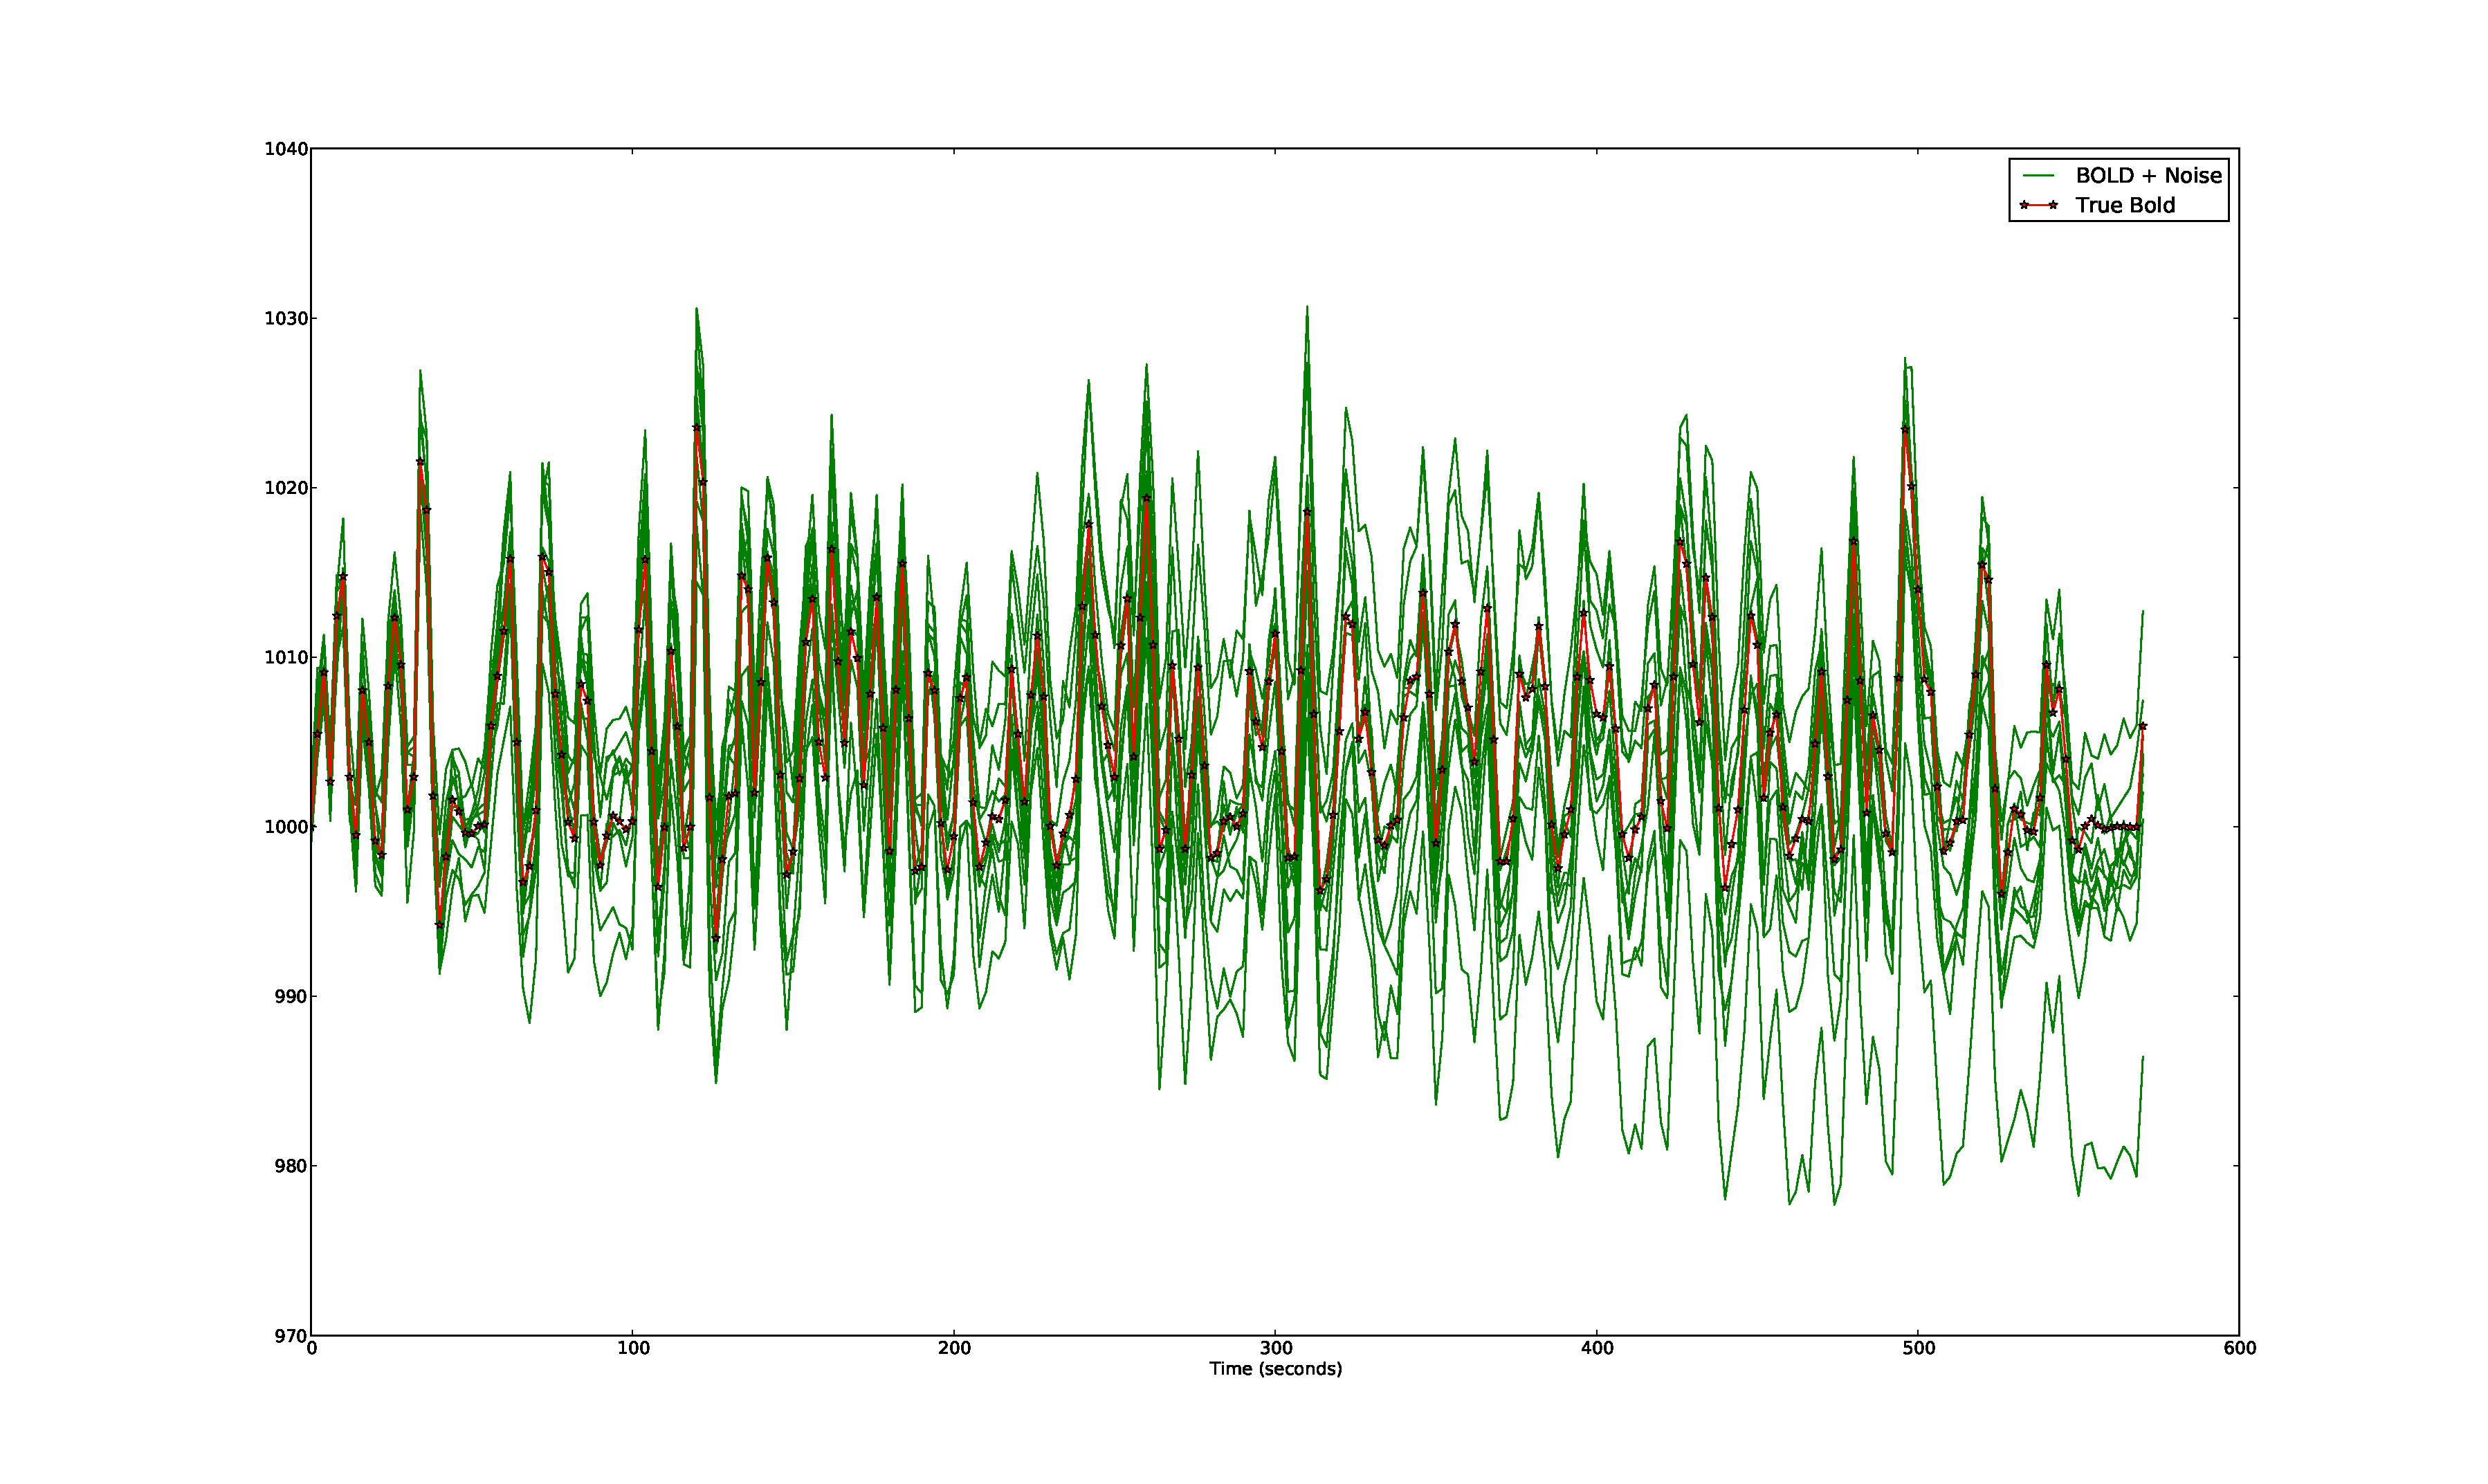
\includegraphics[trim=6cm 3cm 6cm 3cm,width=16cm]{images/realization_lownoise}
\caption{Test Signals with low noise compared to the clean signal}
\end{figure}
The resulting fits compared to the \emph{true} BOLD signal are shown in \autoref{fig:FitComparisonLowNoise}.
While the error between the true signal and the estimated signal are low, the noise
is also relatively low. The actual signal that was delivered into the particle filter
is the result of some preprocessing to remove drift, as described in 
\autoref{sec:Preprocessing}. The preprocessed signal is compared
to the true BOLD signal in \autoref{fig:PreprocessedLowNoise}.
\begin{figure}
\label{fig:PreprocessedLowNoise}
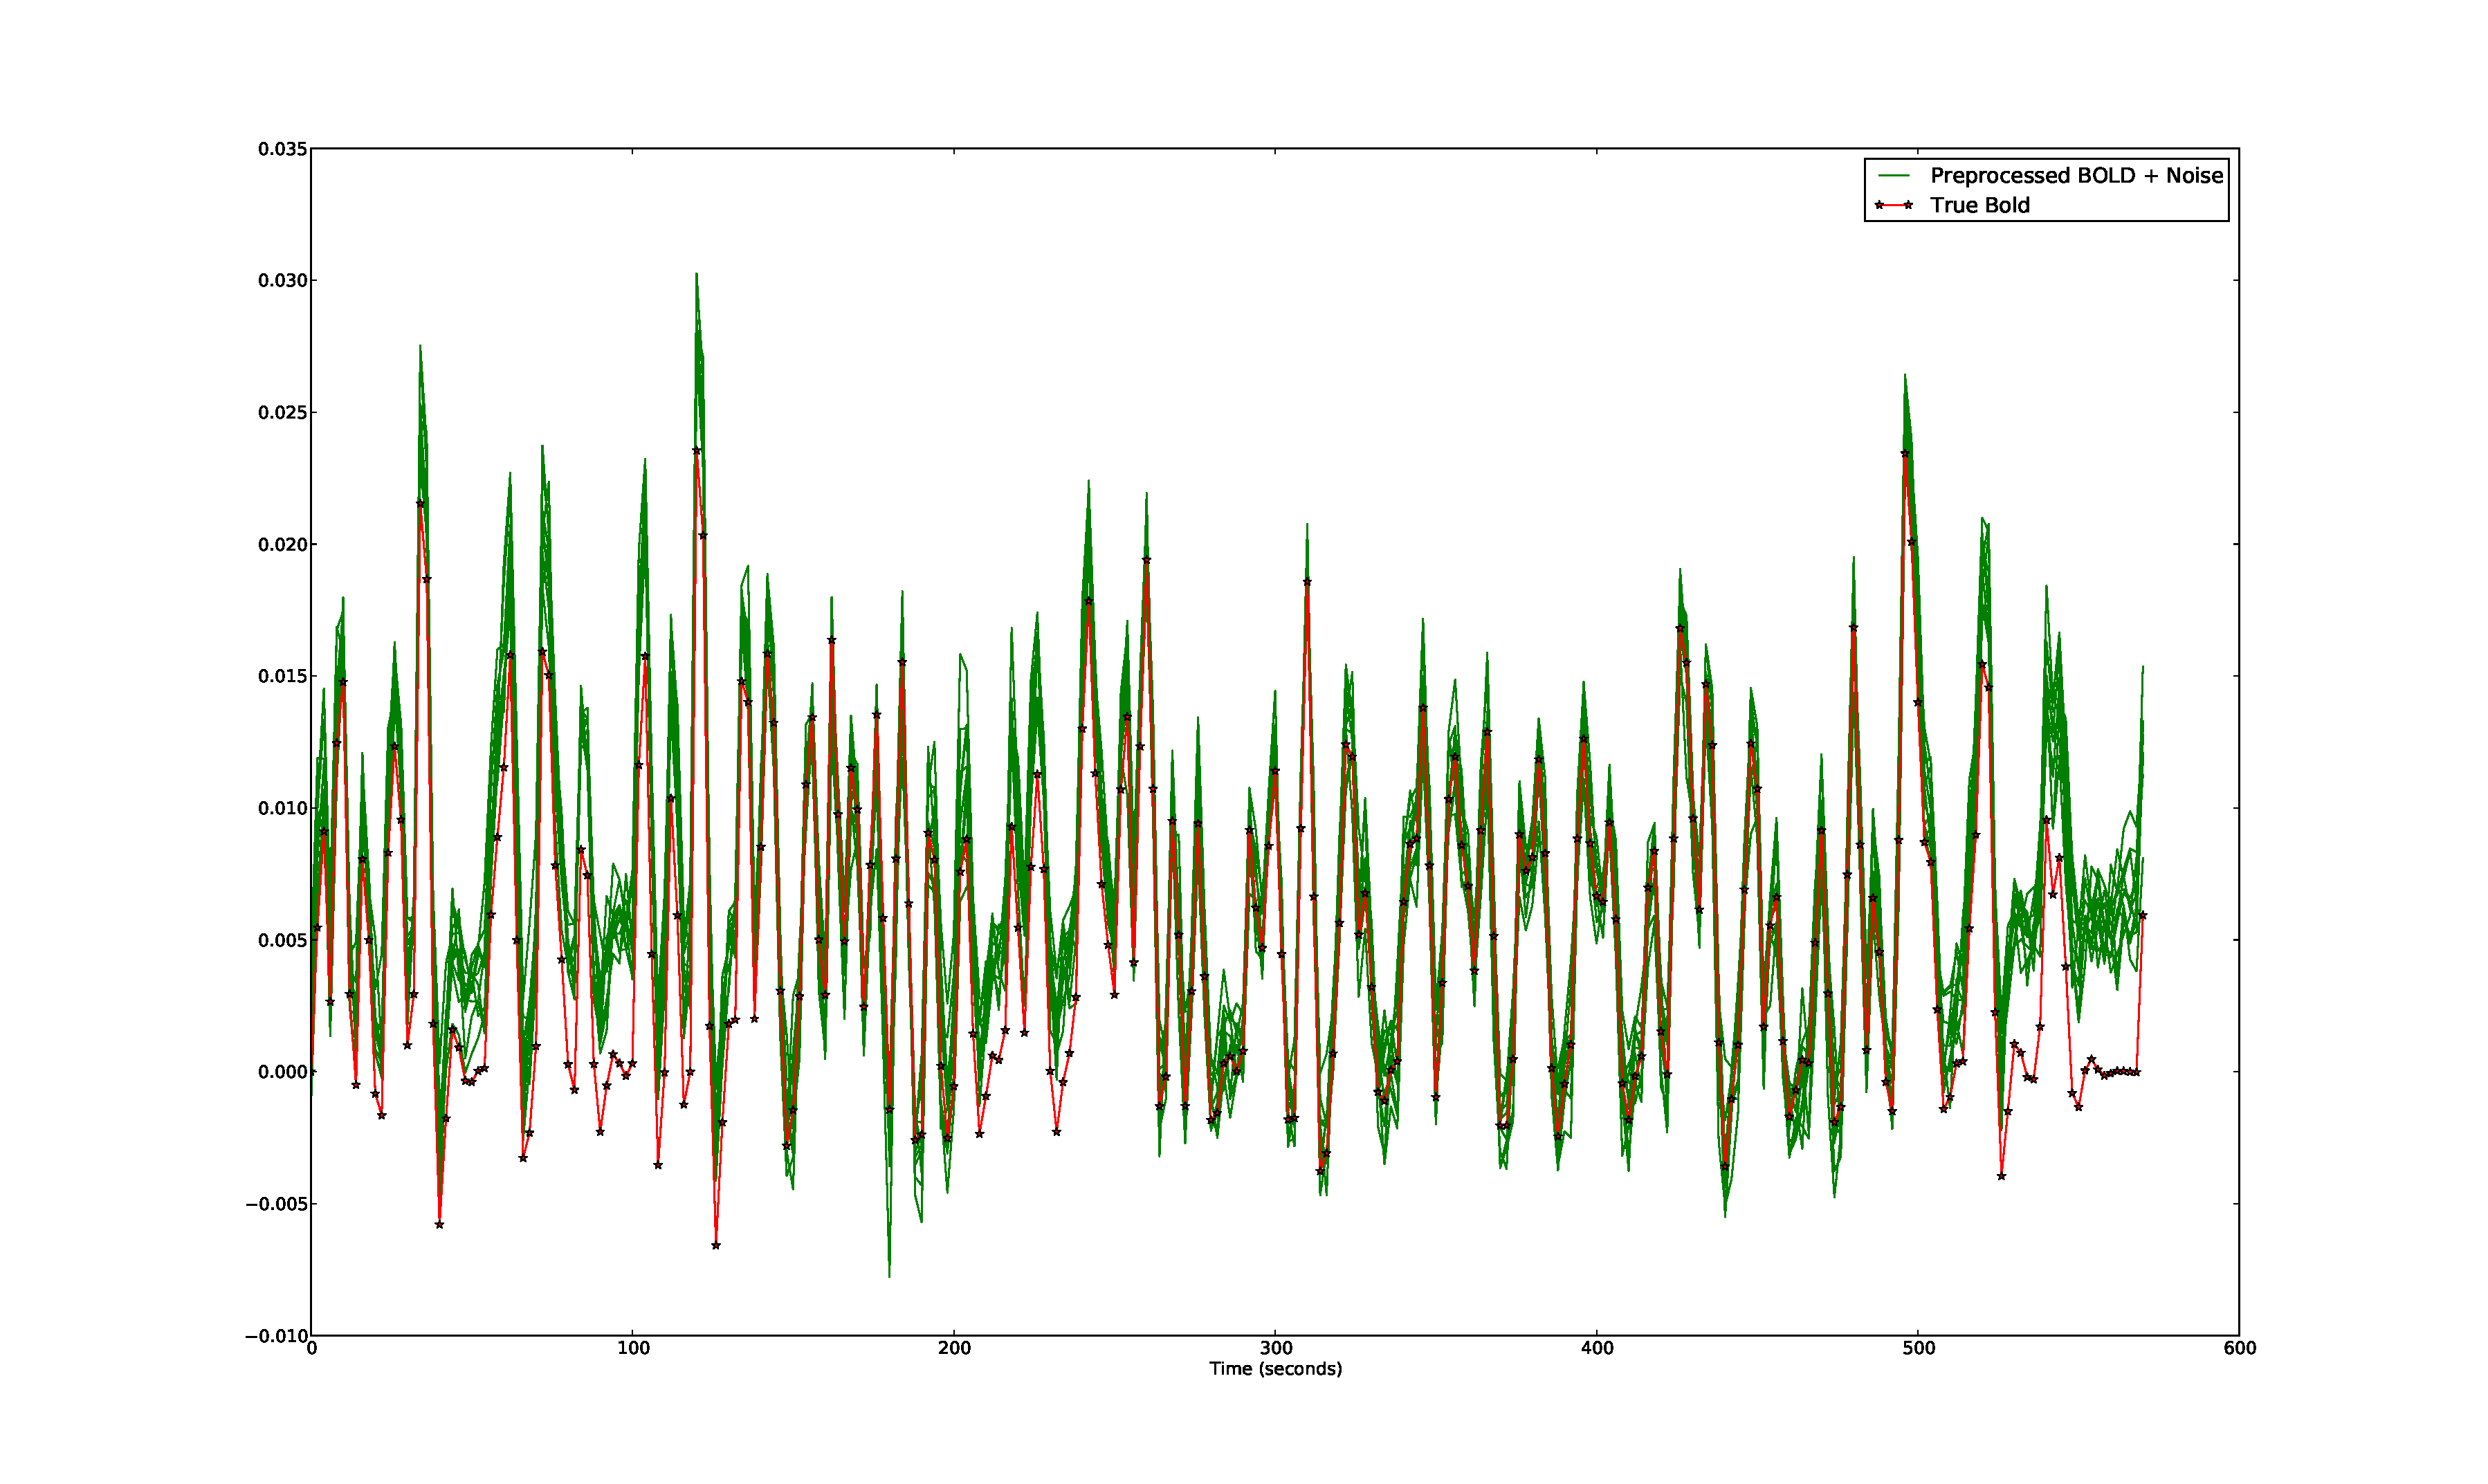
\includegraphics[trim=6cm 3cm 6cm 3cm,width=16cm]{images/preprocessed_lownoise}
\caption{A comparison of the preprocessed signals for the low noise case. This is the
noisy input to the actual particle filter algorithm.}
\end{figure}
The preprocessing consists of several steps, which are discussed in detail in \autoref{sec:Preprocessing}.
Obviously the spline struggles to match the signal near the end, as the graph shows, although 
overall the preprocessing seems to have been successful at removing trends. Finally, the 
set of fits to the preprocessed data, and in 
the true BOLD signal is shown in \autoref{fig:FitComparisonLowNoise}.
\begin{figure}
\label{fig:FitComparisonLowNoise}
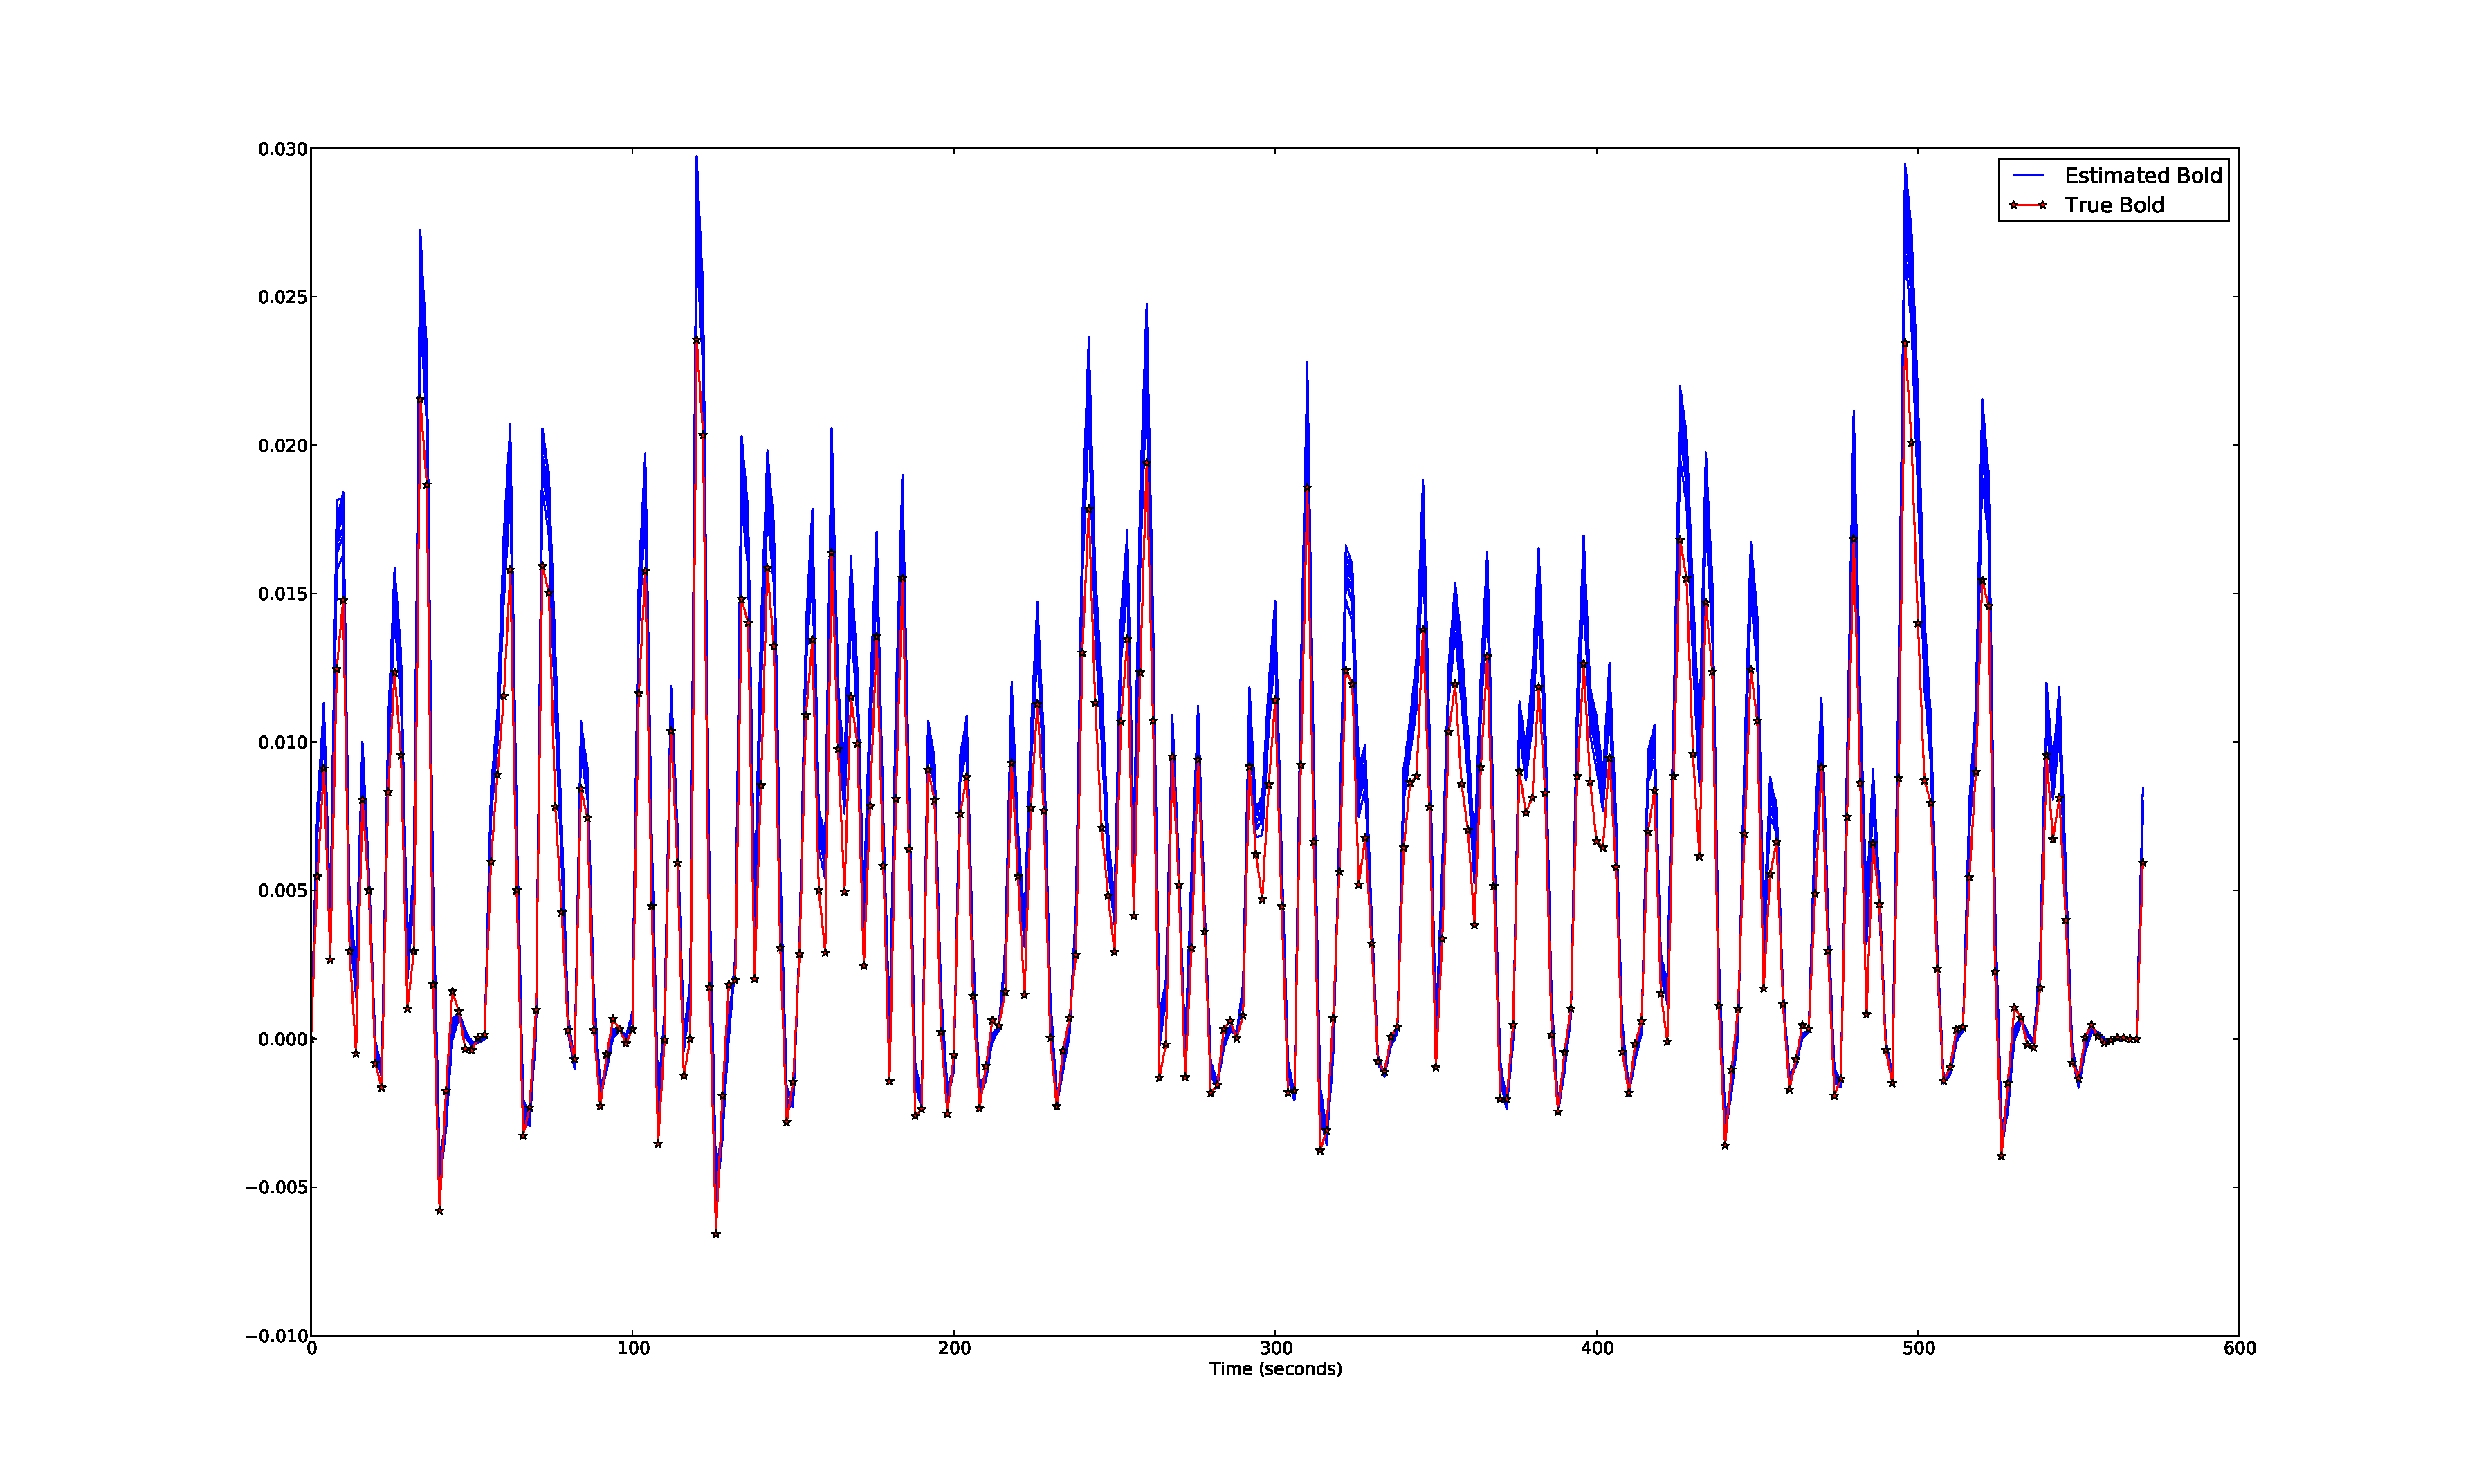
\includegraphics[trim=6cm 3cm 6cm 3cm,width=16cm]{images/comparison_lownoise}
\caption{A comparison of the fitted signals for the low noise case.}
\end{figure}
The filtering property of the particle filter is clear from the results here.  In several locations the output
of the particle filter looks like a filtered version of the input. For instance toward the
end, the estimates stay flat in spite of the preprocessed data drifting off a bit. By
this point, the algorithm had converged sufficiently to know that that such a movement in
signal isn't possible. A similar circumstance occurs at 100 seconds in. 
In general the fits are good, although because
of the slightly higher signal levels in the preprocessed signals, the fits tend to overestimate
the peaks. The final parameter sets are shown in \autoref{tab:LowNoiseParams}
\begin{table}[t]
\centering
\begin{tabular}{|c | c | c | c | c | c | c | c | c | c |}
\hline 
$\tau_0$ & $\alpha$ & $E_0$    & $V_0$    & $\tau_s$ & $\tau_f$ & $\epsilon$  & $ \sum \tau $ & $\sqrt{MSE}$ (Res.) &$\sqrt{MSE}$\\
\hline 
\rowcolor[gray]{.8}
1.45 & .3 & .47 & .044 & 1.94 & 1.99 & 1.8  & 5.38 &  & \\
\hline 
\hline 
1.22214 & 0.3449 & 0.33462 & 0.07138 & 1.60446 & 2.27529 & 1.59454 & 5.10189  &  0.00321067  & 0.00987647  \\
1.37493 & 0.33183 & 0.36296 & 0.07327 & 1.64076 & 2.10299 & 1.57627 & 5.11867 &  0.00305475  & 0.00993227  \\
1.16604 & 0.32205 & 0.34057 & 0.08217 & 1.64768 & 2.35351 & 1.24515 & 5.16722 &  0.00328932  & 0.00967961  \\
1.23176 & 0.32707 & 0.34028 & 0.07961 & 1.62698 & 2.18519 & 1.30326 & 5.04394 &  0.00284719  & 0.00912005  \\
1.1832 & 0.31787 & 0.34718 & 0.0821 & 1.54961 & 2.29115 & 1.27817 & 5.02396   &  0.00300634  & 0.00971258  \\
1.1424 & 0.33395 & 0.34725 & 0.07366 & 1.62208 & 2.29084 & 1.4025 & 5.05531   &  0.00283287  & 0.00948483  \\
1.30041 & 0.3596 & 0.35643 & 0.07679 & 1.56406 & 2.13234 & 1.60338 & 4.99681  &  0.00302802  & 0.01021885  \\
1.24008 & 0.34601 & 0.33978 & 0.08903 & 1.64989 & 2.23655 & 1.29004 & 5.12651 &  0.00304378  & 0.01007964  \\
1.1709 & 0.32739 & 0.34644 & 0.08255 & 1.53734 & 2.28262 & 1.37828 & 4.99087  &  0.00334488  & 0.01032886  \\
1.18967 & 0.34344 & 0.33554 & 0.07976 & 1.53582 & 2.30746 & 1.42774 & 5.03295 &  0.00317542  & 0.01001503  \\
1.184 & 0.34053 & 0.35017 & 0.08917 & 1.61025 & 2.27926 & 1.16448 & 5.07352   &  0.00288855  & 0.00950536  \\
\hline                                                                           
1.21868 & 0.33588 & 0.34557 & 0.07995 & 1.59899 & 2.24884 & 1.38762 & 5.06651 & 0.00306562     & 0.00981396 \\
\hline 
\end{tabular}
\caption{Estimated Parameters on 11 different runs with low noise. First row is the true parameters,
last is mean over the 10 runs. The $\sqrt{MSE}$ (Res.) is the square root of the mean square of the
residuals. Essentially this is the is the MSE between the estimated signal and the noisy signal which 
was available to the particle filter. Square root of MSE is the actual \emph{error}, with the true signal,
which of course was not available to the particle filter.}
\label{tab:LowNoiseResults} 
\end{table}
There are a few results worth noting here. First the time constants vary greatly across
runs with different noise realizations, yet the sum of the individual time constants
($\tau_f$, $\tau_s$ and $\tau_0$) seem to be more consistent. In general the 
time constants are falling short of the true time constant. This could be a limitation
based on the prior distribution (which notably has an initial mean below the values used
in the simulation) or it could be caused by the dissassociated benefits of a correct time
constant with correct output. It often takes several measurement periods before a difference
in time constants becomes relevent. It is possible that in that time other parameters 
may be more relevent. As a result, by the time the time constant has made a substantial
difference in the weight, the 
particle with the better $\tau$ will have been weighted based on other parameters several
times. Another interesting result in the huge variation in the levels of $V_0$. In general,
with this admittedly small amount of noise, it would appear that the relation between a set
of parameters/stimuli and the output is not injective. In other words, it would appear
that a timeseries is not unique to a single set of parameters. This is good justification that 
simultaneous blood volume or tagged flow calculations with the conventional FMRI 
could definitely benefit the model. 
\begin{table}[t]
\centering
\begin{tabular}{|c | c  c  c  c  c  c  c |}
\hline 
  & $\tau_0$ & $\alpha$ & $E_0$    & $V_0$    & $\tau_s$ & $\tau_f$ & $\epsilon$ \\
\hline 
\rowcolor[gray]{.8} $\tau_0$ &   0.0189481 & -0.0014269 & -0.0011267 & -1.13e-05 & -0.0025616 & -0.0189559 & 0.0070405 \\
$\alpha$ &                       -0.0014269 & 0.0026716 & 9.93e-05 & -0.0002041 & -0.0008632 & -0.0016823 & 0.0071891 \\
\rowcolor[gray]{.8} $E_0$    &   -0.0011267 & 9.93e-05 & 0.0010701 & -0.0002277 & -0.0001177 & 0.0001013 & 0.0016972 \\
$V_0$    &                       -1.13e-05 & -0.0002041 & -0.0002277 & 0.0005401 & 4.3e-06 & 4.56e-05 & -0.0080494 \\
\rowcolor[gray]{.8} $\tau_s$ &   -0.0025616 & -0.0008632 & -0.0001177 & 4.3e-06 & 0.0128056 & 0.012878 & -0.005516 \\
$\tau_f$ &                       -0.0189559 & -0.0016823 & 0.0001013 & 4.56e-05 & 0.012878 & 0.0416927 & -0.0158182 \\
\rowcolor[gray]{.8} $\epsilon$&  0.0070405 & 0.0071891 & 0.0016972 & -0.0080494 & -0.005516 & -0.0158182 & 0.1567165 \\
\hline 
\end{tabular}
\caption{Typical Covariance matrix of the parameters at the end of a run.}
\label{tab:CovSim} 
\end{table}

\begin{figure}[H]
\subfigure[Converging histogram for $\tau_0$, $\alpha$, $E_0$, and $V_0$ of the first run, low noise simulation.]
{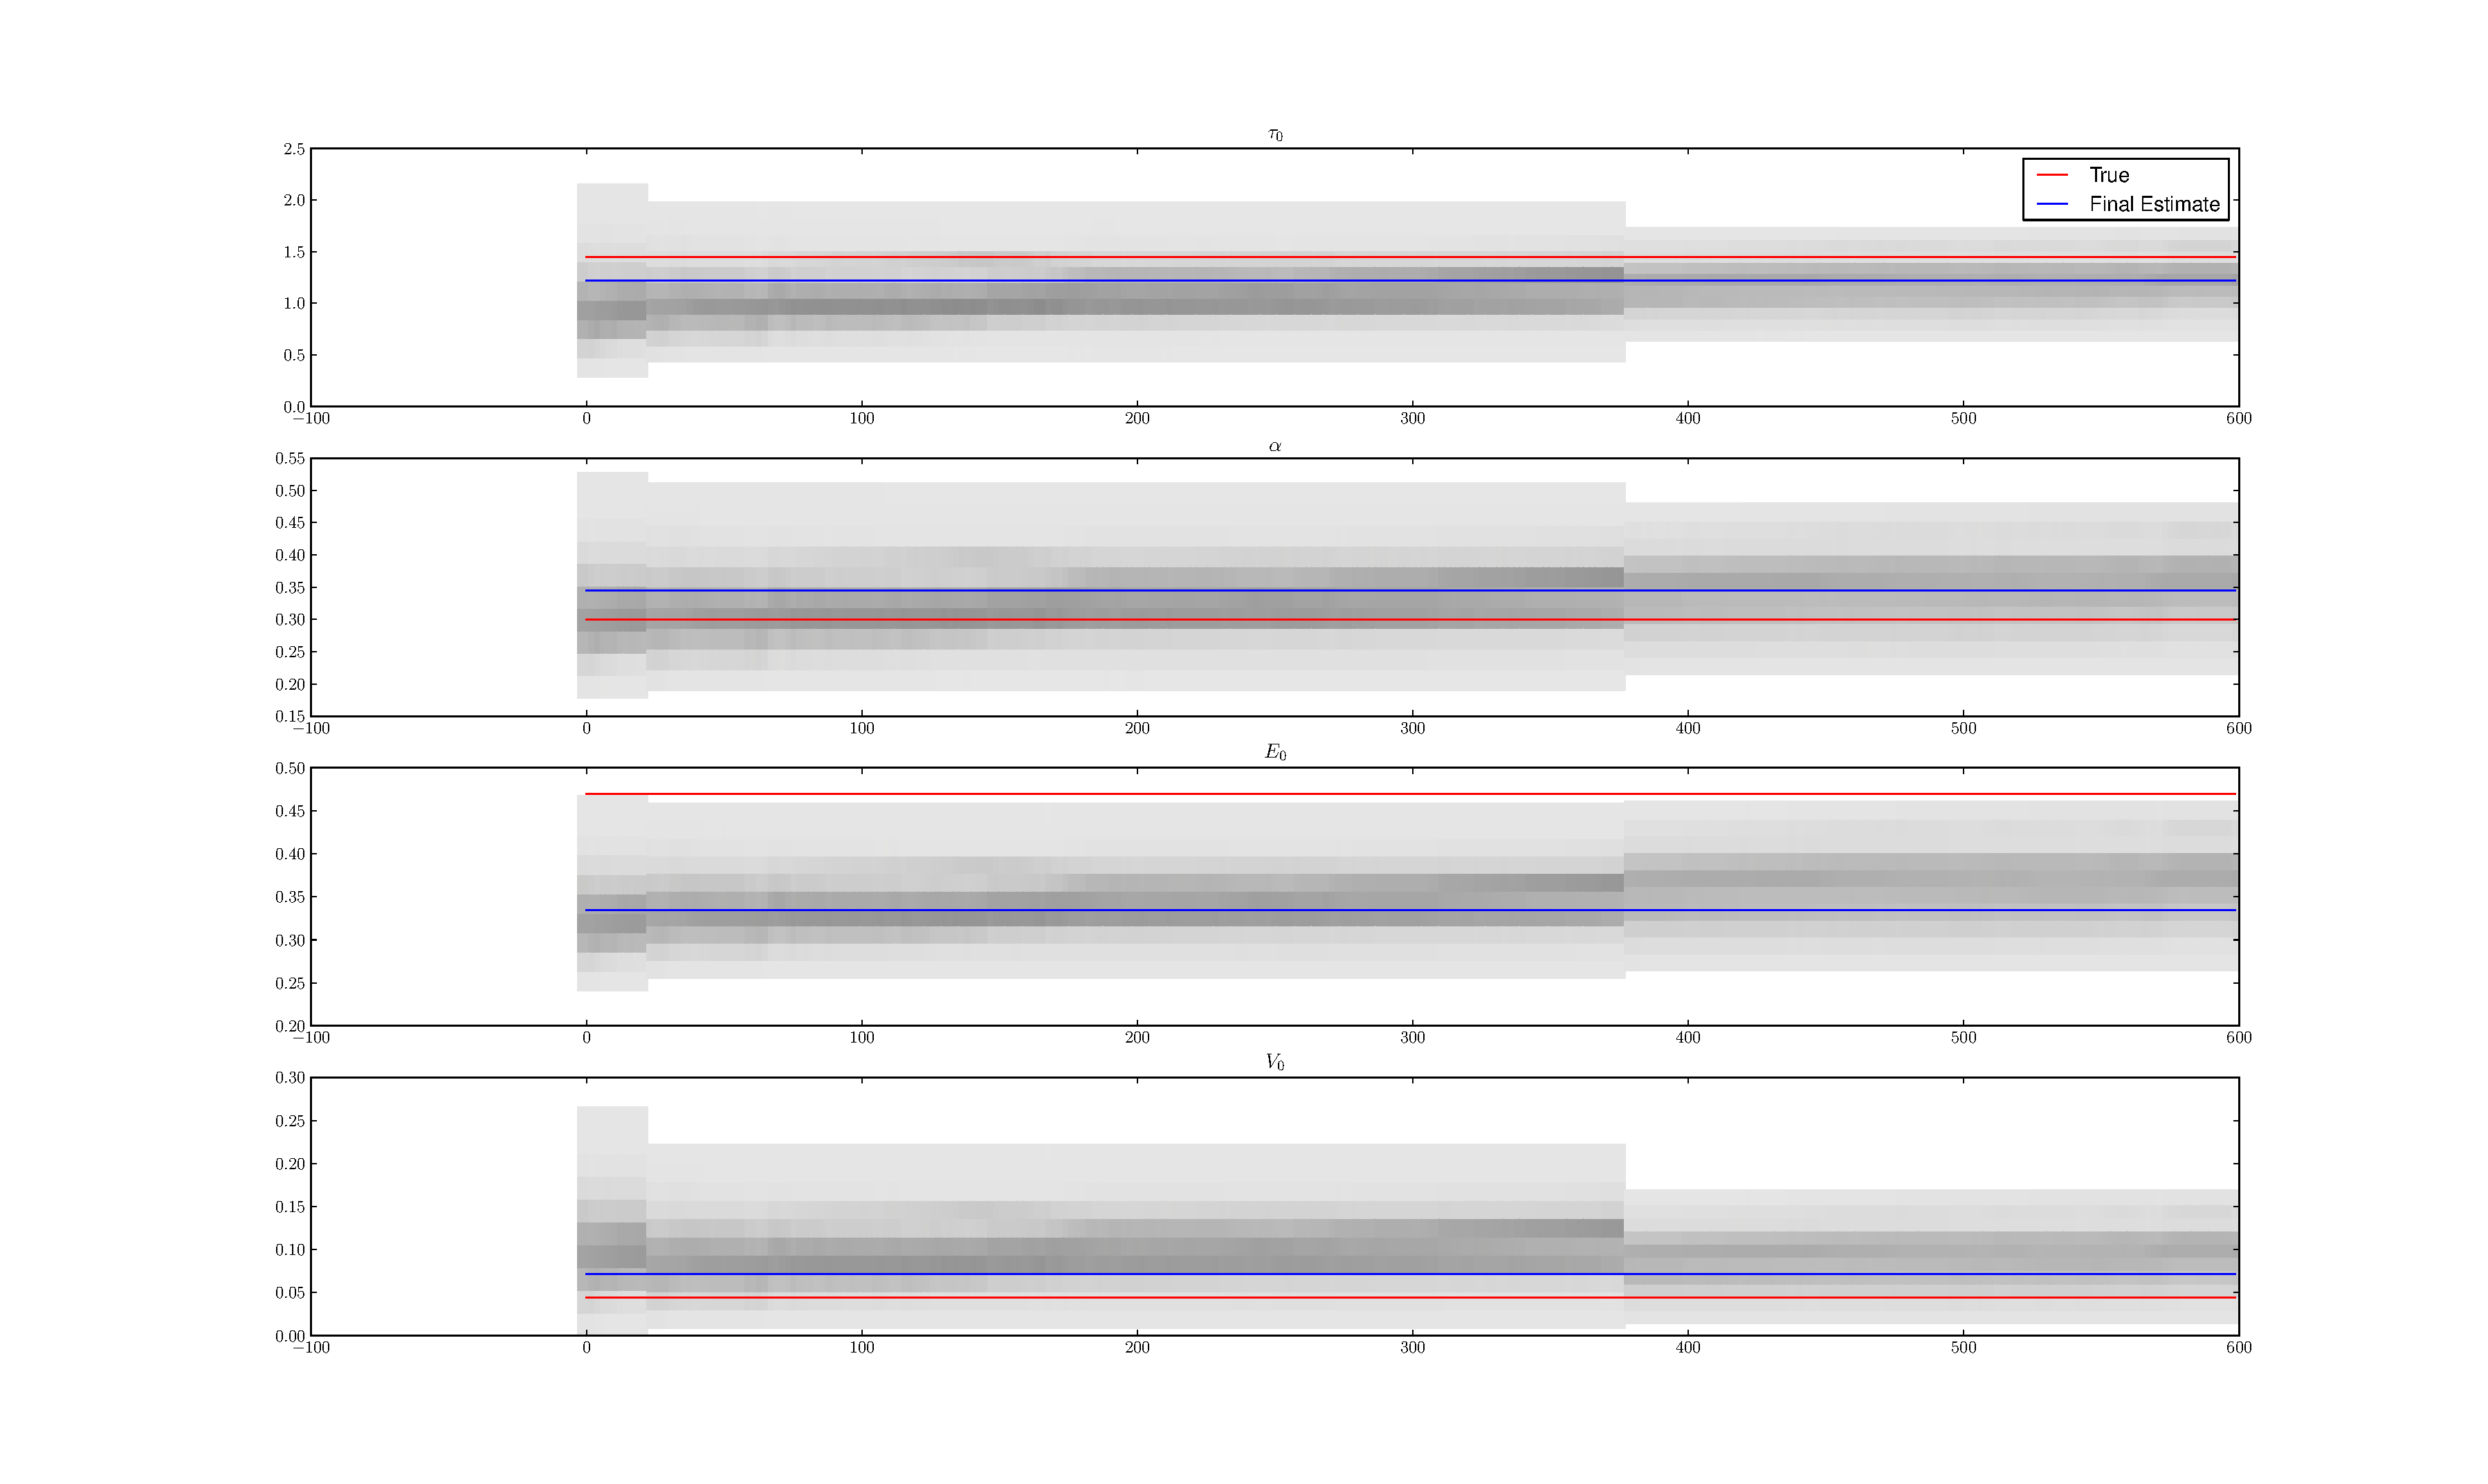
\includegraphics[trim=7cm 4cm 7cm 4cm, width=15cm]{images/converge_lownoise1}}\\

\subfigure[Converging histogram for $\tau_s$, $\tau_f$, $\epsilon$, and $V$ of the first run, low noise simulation.]
{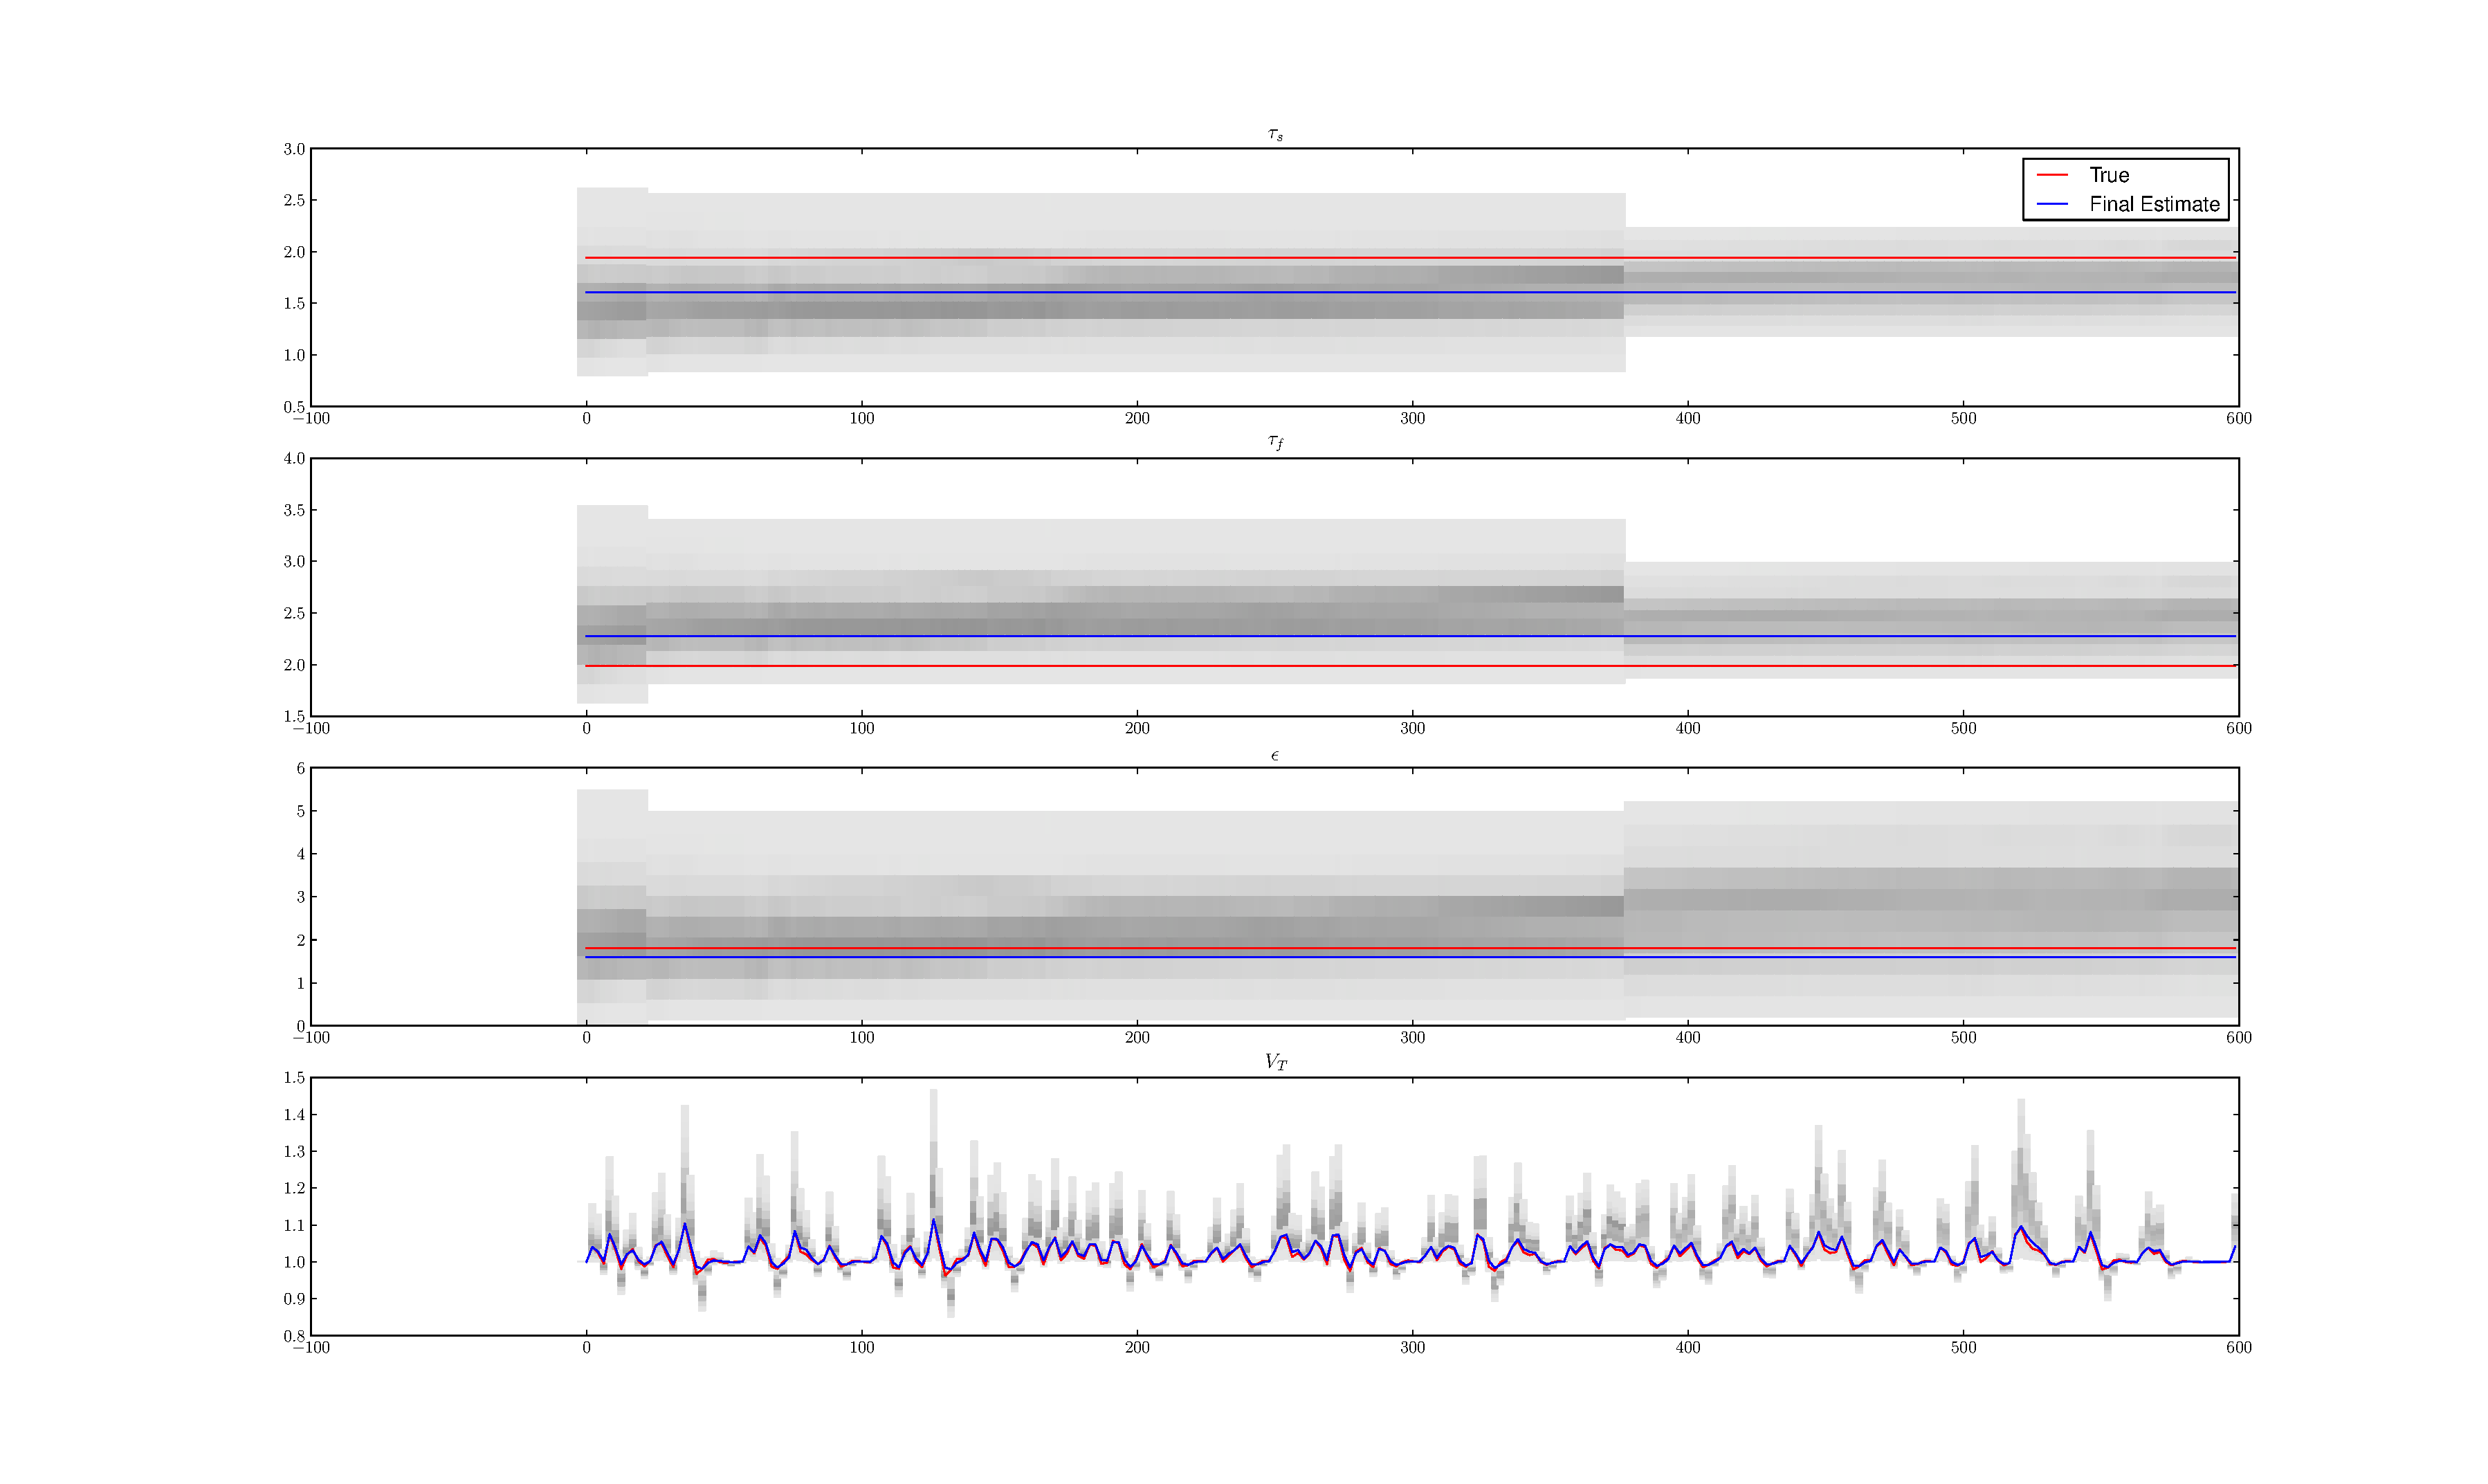
\includegraphics[trim=7cm 4cm 7cm 1cm, width=15cm]{images/converge_lownoise2}}\\
\end{figure}

\begin{figure}
\subfigure[Converging histogram for $Q$, $S$, $F$, and $BOLD$ of the first run, low noise simulation.]
{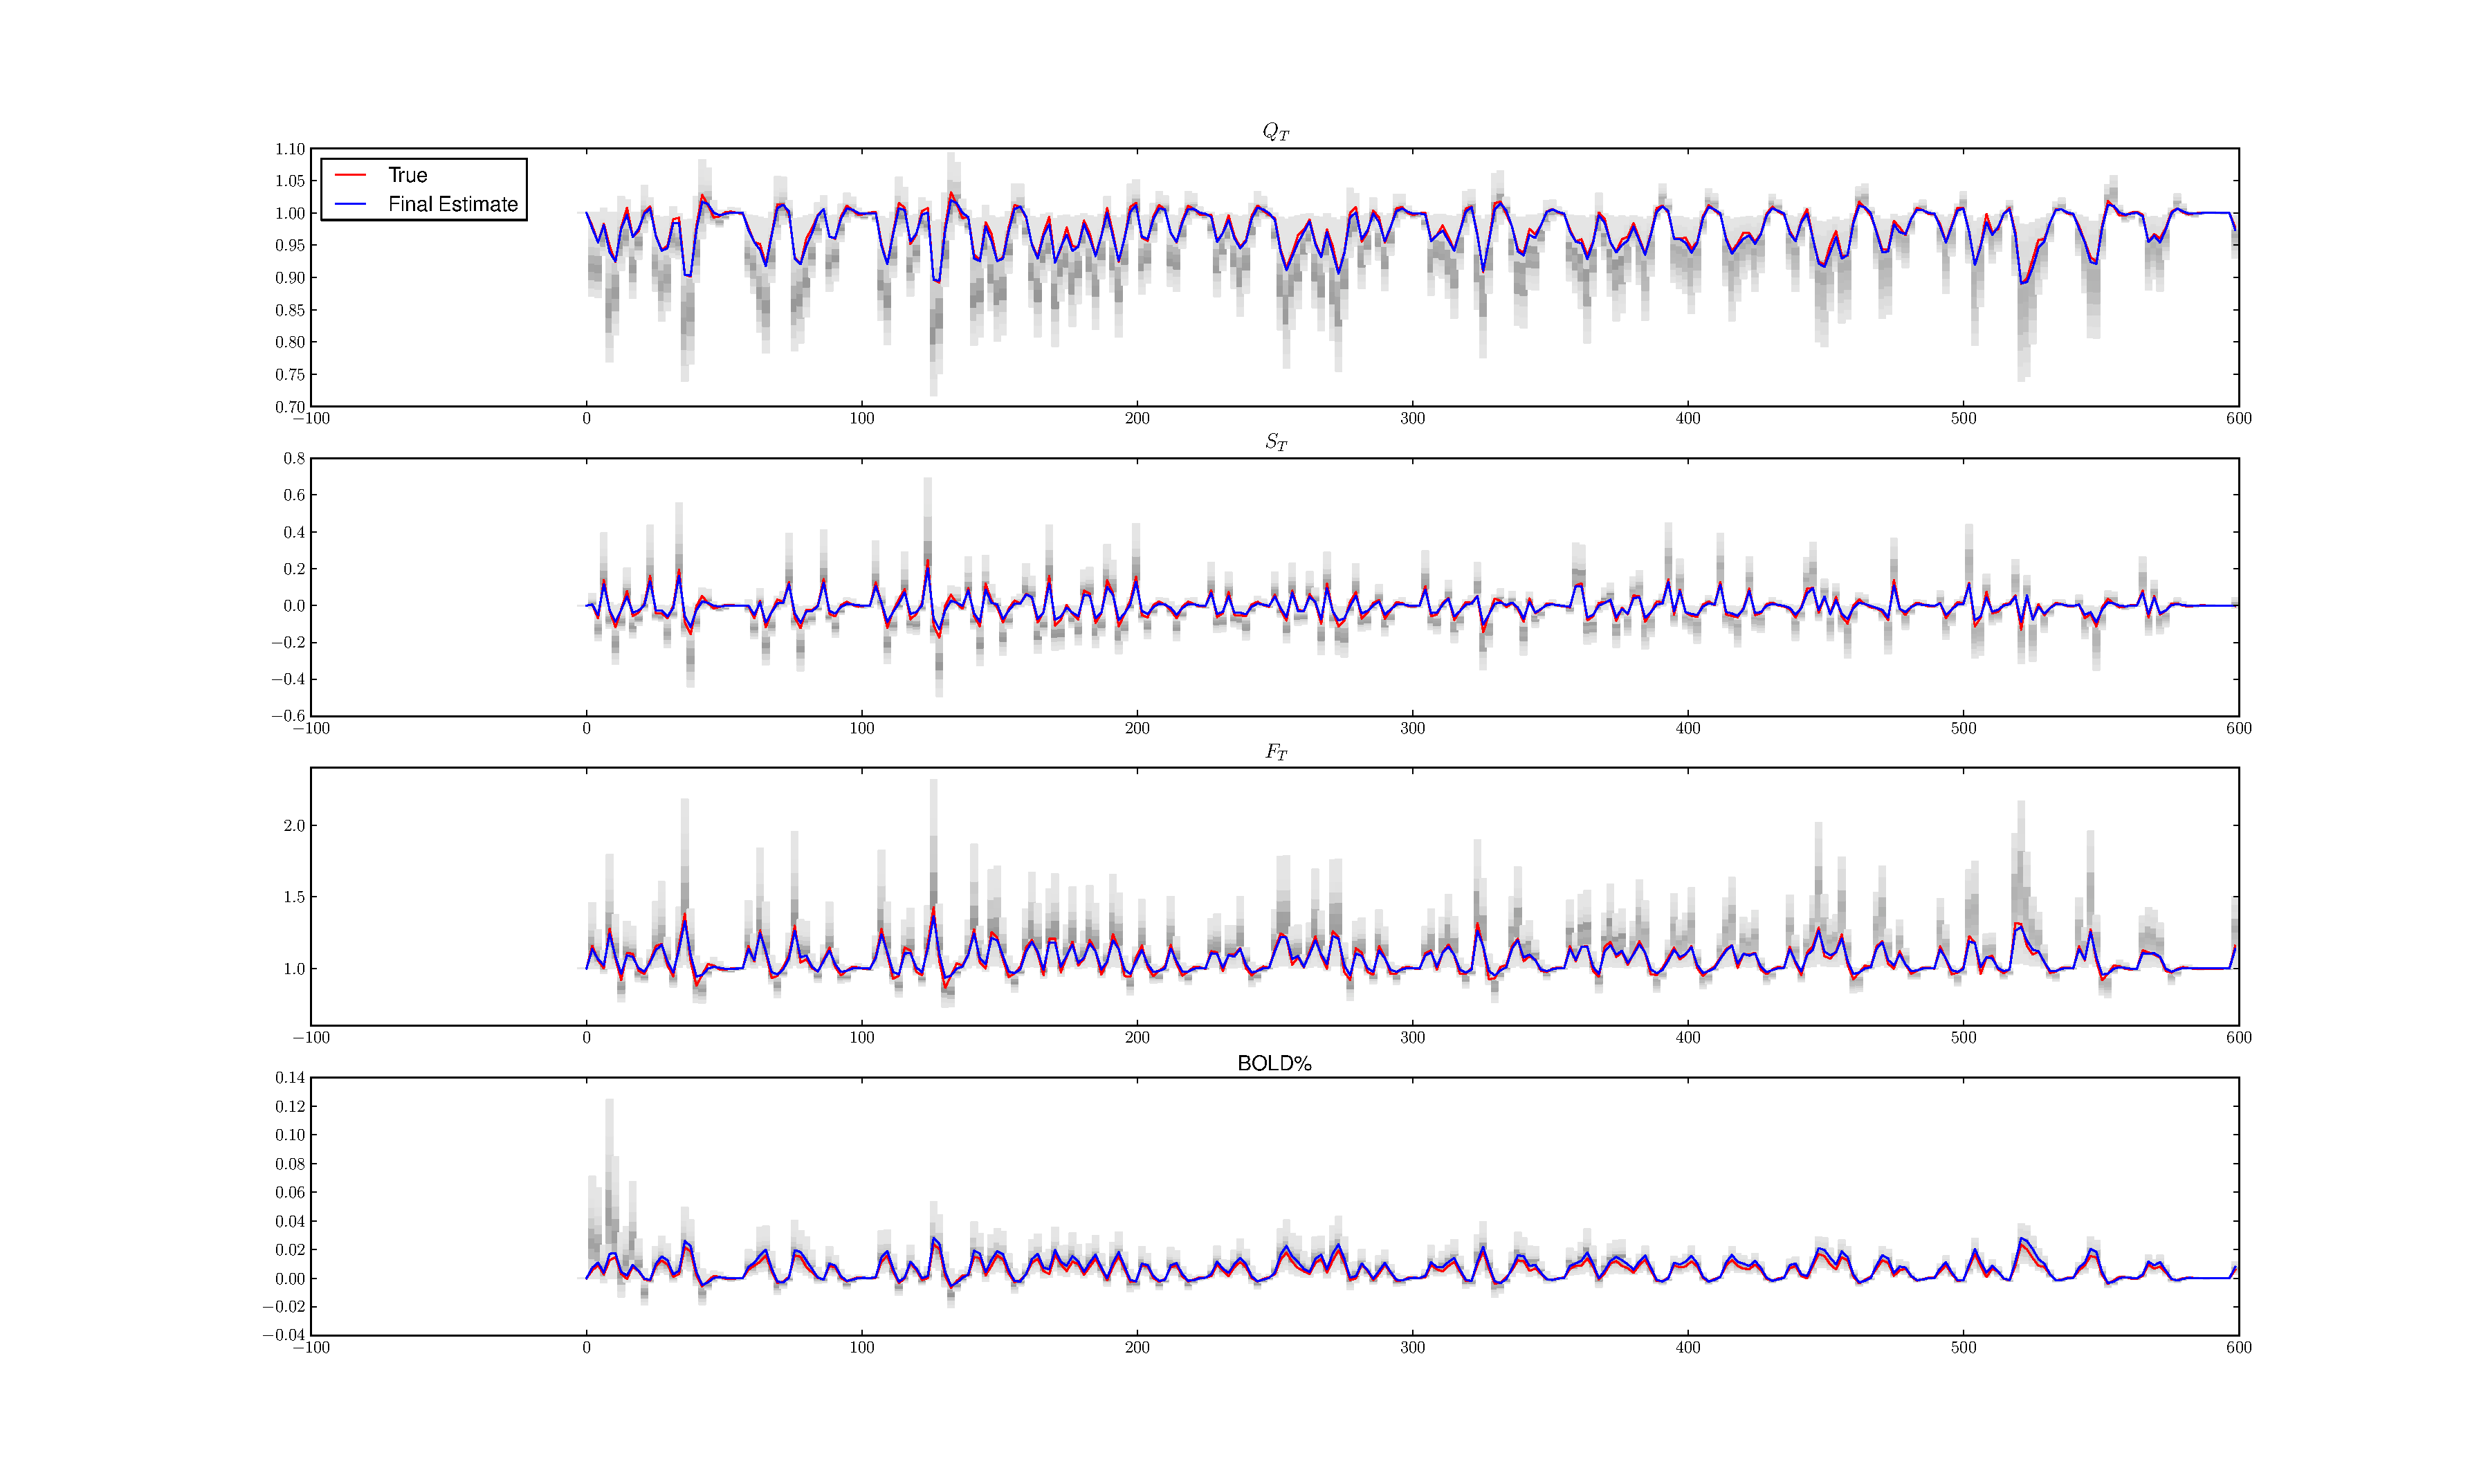
\includegraphics[trim=7cm 2cm 7cm 2cm, width=15cm]{images/converge_lownoise3}}
\label{fig:LowNoiseHist}
\end{figure}
The covariance matrix (\autoref{tab:CovSim}) also confirms the idea that the $\tau$ parameters are interchangeable
as far as the BOLD signal goes. Notice the covariance of $\tau_f$ and $\tau_0$ is $-0.019$ whereas
the variance of $\tau_0$ and $\tau_f$ are $0.019$ and $0.04$ respectively. Clearly there is 
some measure of ill-defined behavior between the differen time-constants, as well as several
other variables.  The convergence properties of the first run in \autoref{tab:LowNoiseResults} may be
viewed in \autoref{fig:LowNoiseHist}.

TODO more about convergence

\subsection{High Noise}
\label{sec:HighNoise}
For the high noise simulation, the exact same procedure was performed again, but with 
measurement error and drift standard
deviations an order of magnitude higher. The noisy signals versus the base signal are shown
in \autoref{fig:HighNoiseRealization} and the preprocessed signals which the particle
filter attempt to fit are in \autoref{fig:PreprocessedHighNoise}.
\begin{figure}[H]
\label{fig:LowNoiseRealization}
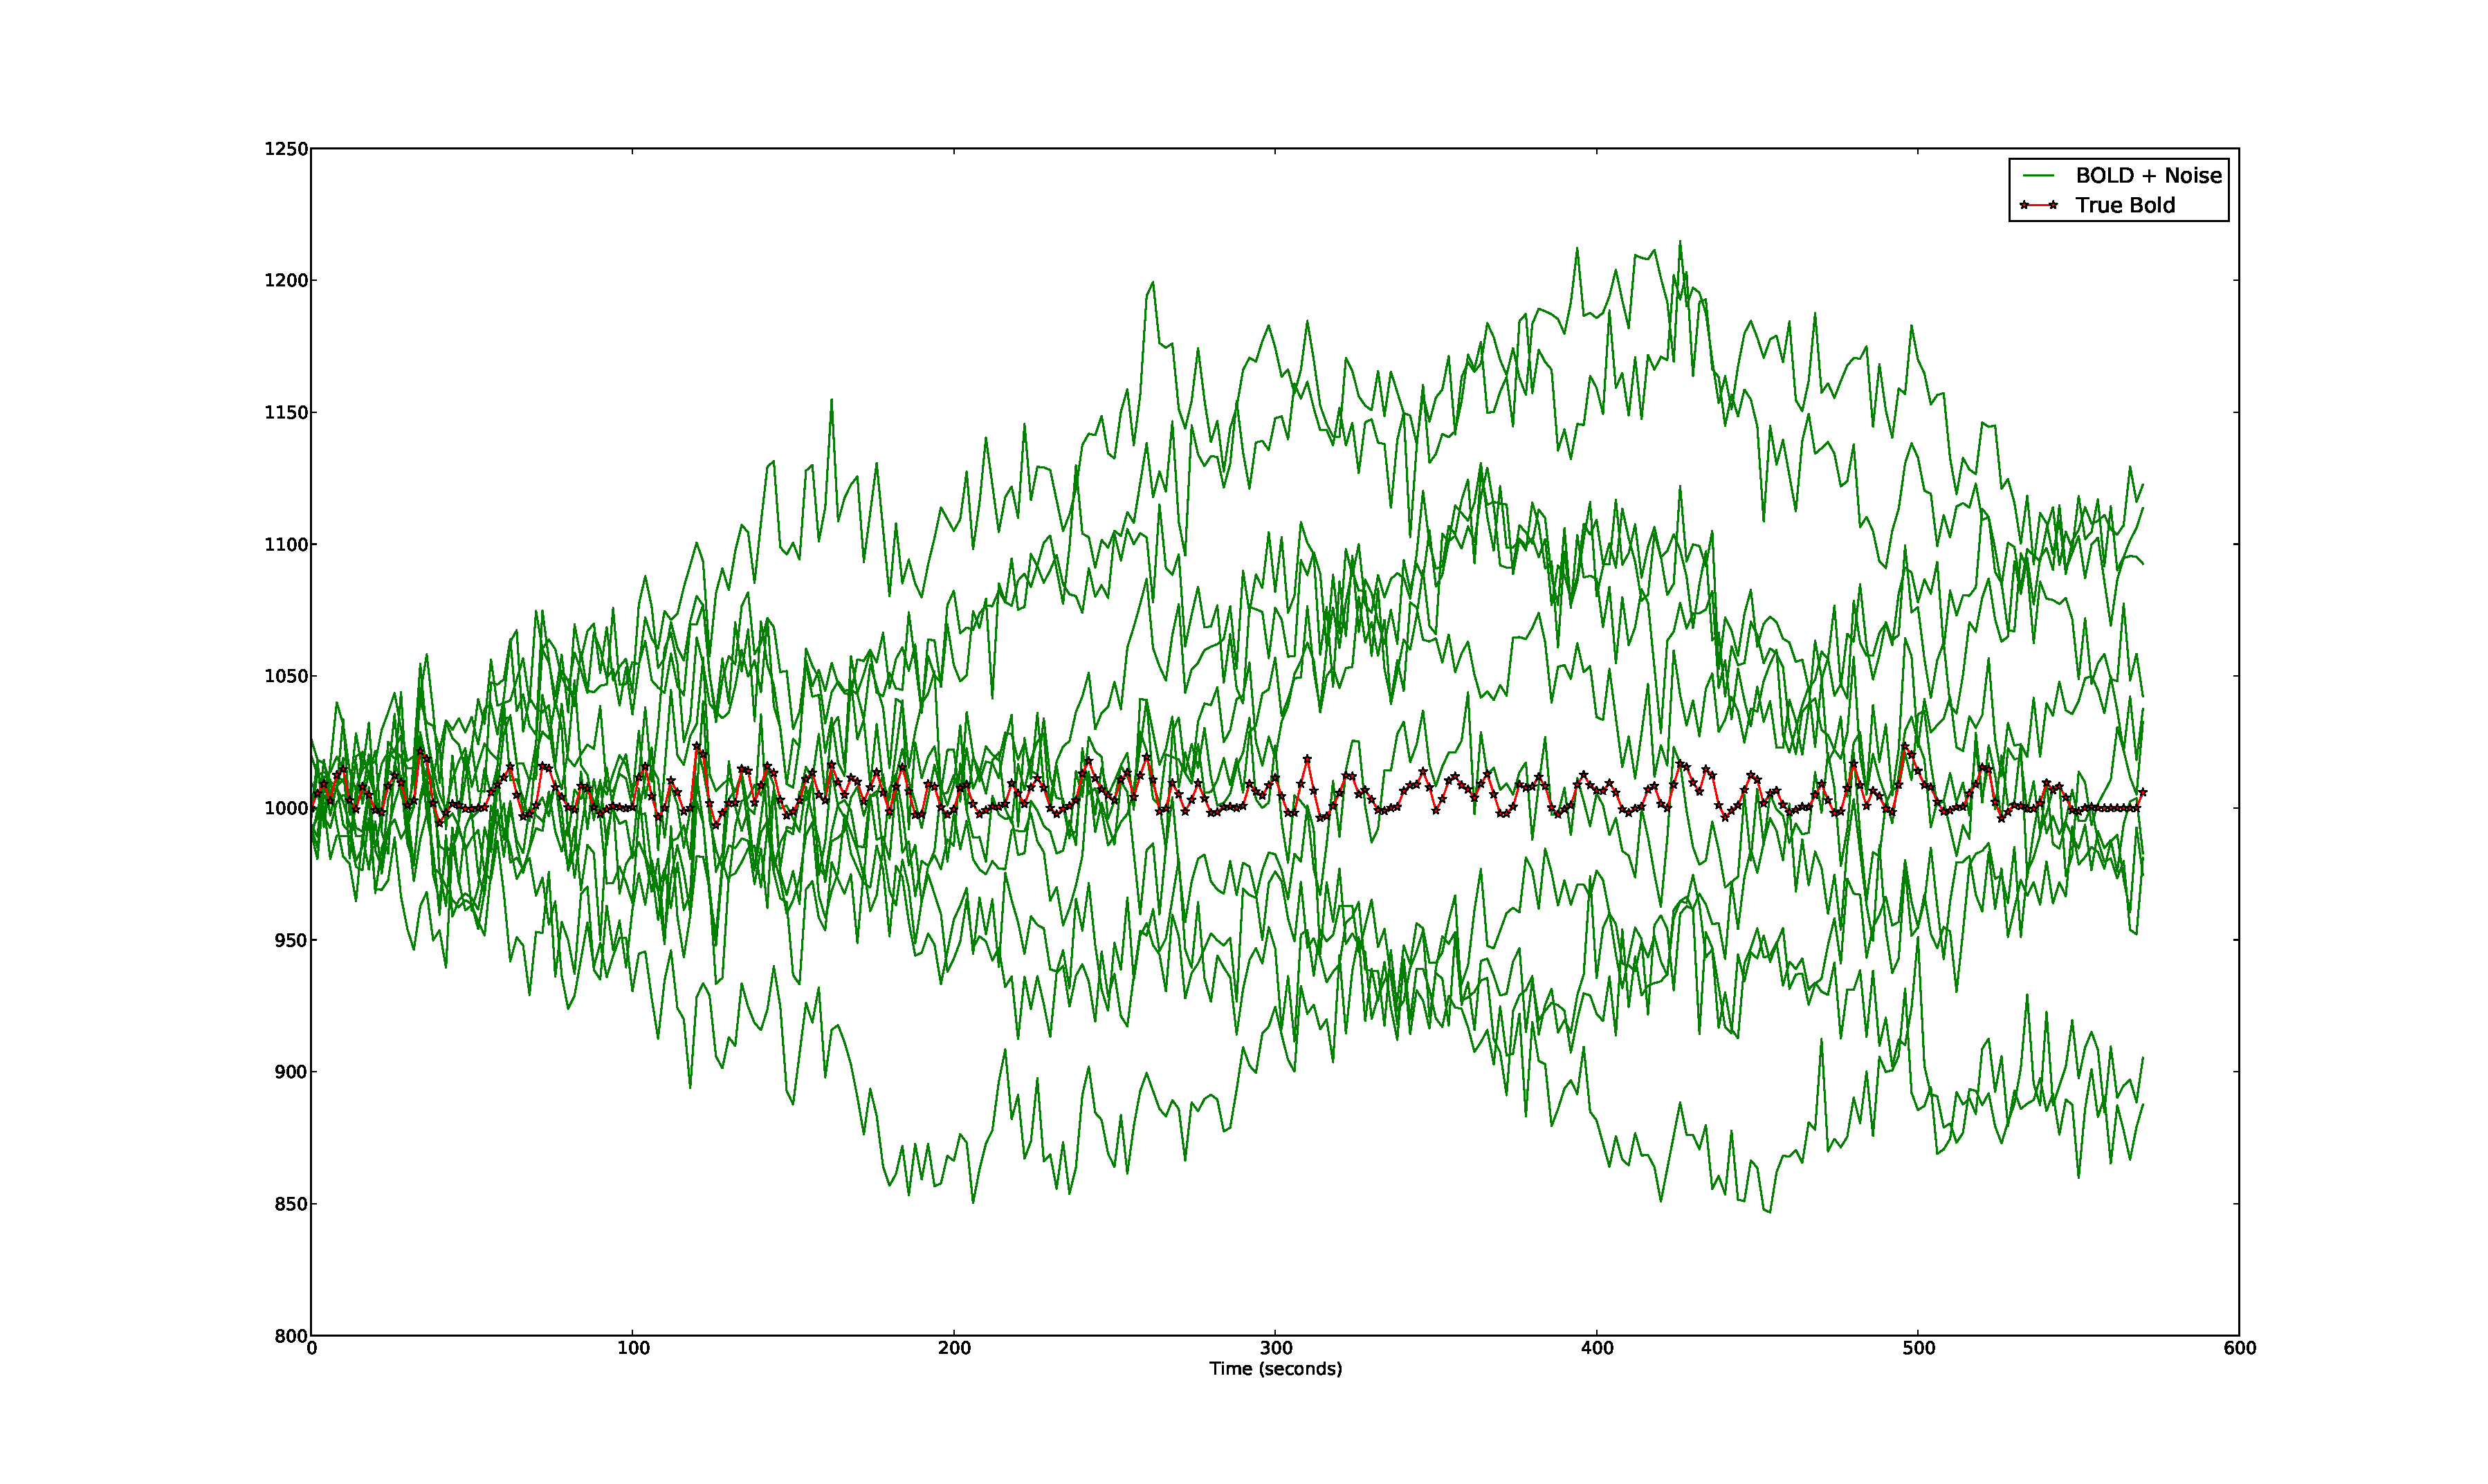
\includegraphics[trim=6cm 3cm 6cm 3cm,width=16cm]{images/realization_highnoise}
\caption{Test Signals with high noise compared to the clean signal, $\sigma_x = .01, \sigma_y=.005$}
\end{figure}
\begin{figure}[H]
\label{fig:PreprocessedHighNoise}
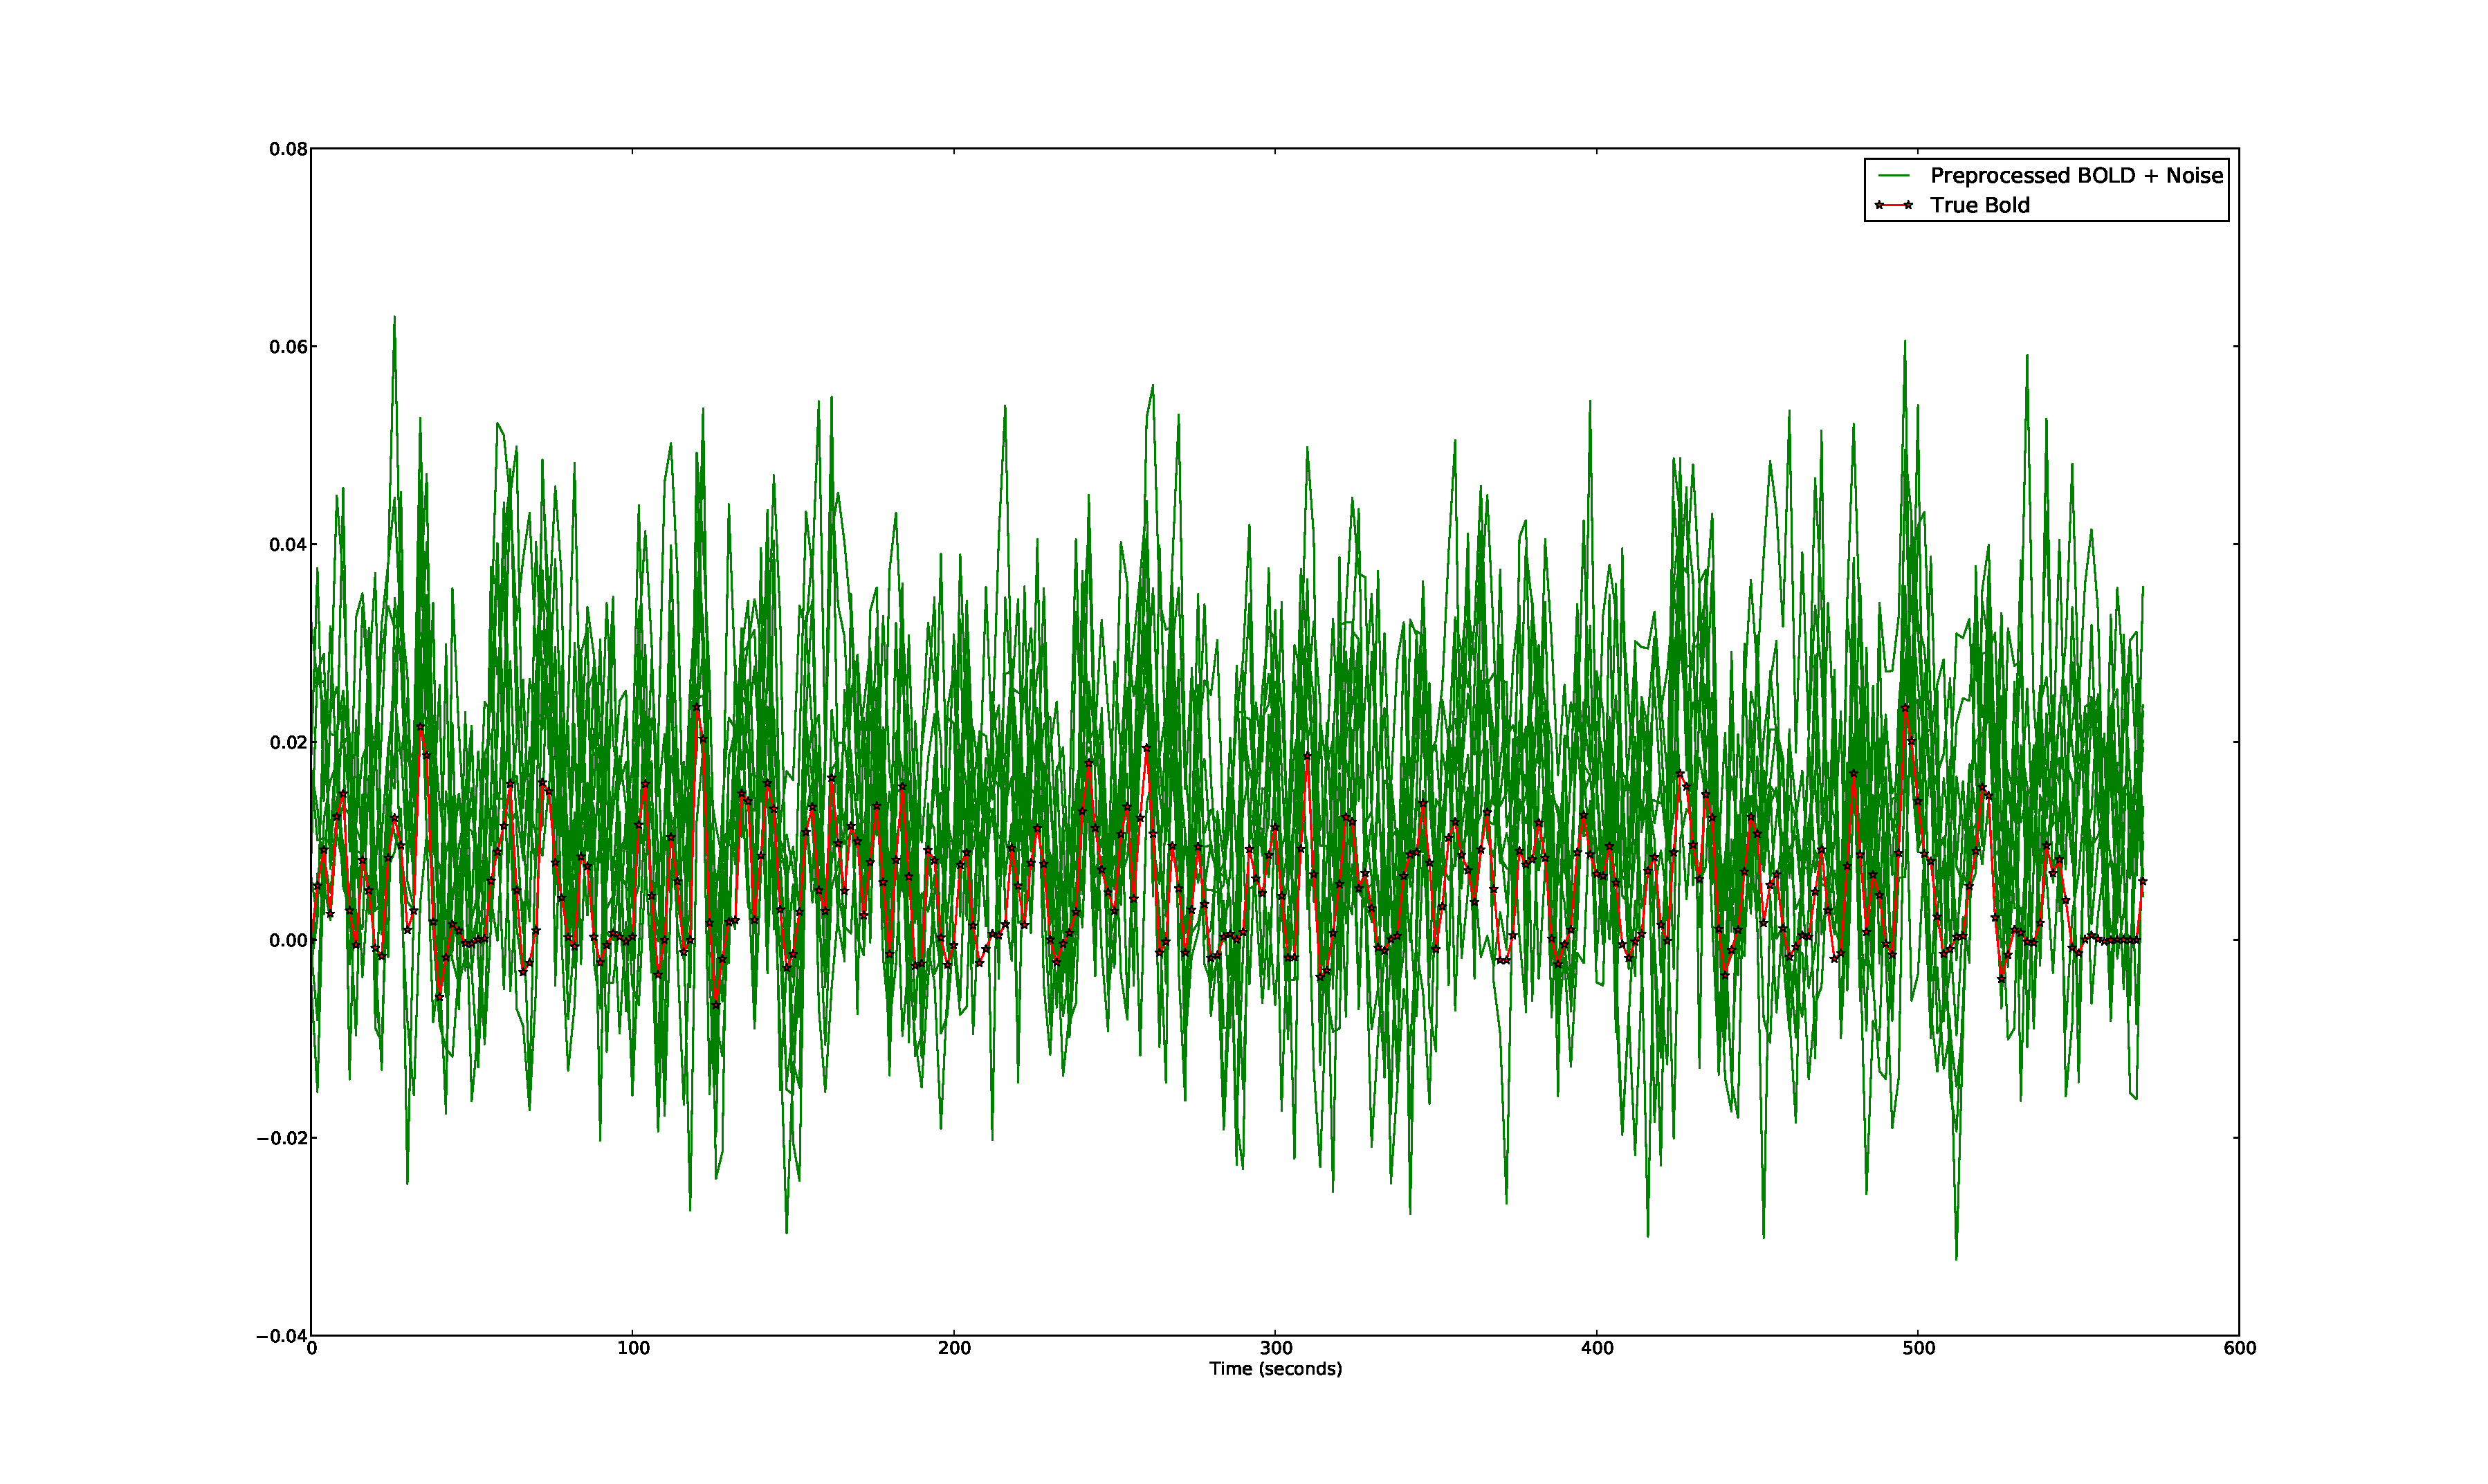
\includegraphics[trim=6cm 3cm 6cm 3cm,width=16cm]{images/preprocessed_highnoise}
\caption{A comparison of the preprocessed signals for the high noise case.}
\end{figure}

The results of the particle filter, for each of the ten runs may be seen in 
\autoref{fig:FitComparisonHighNoise}. Clearly the preprocessing led the algorithm
to somewhat higher activation levels, and it would appear that the subtleties of
different time constants are also lost for most of the runs, although a few seem
to manage quite accurate results. 

\begin{figure}[H]
\label{fig:FitComparisonHighNoise}
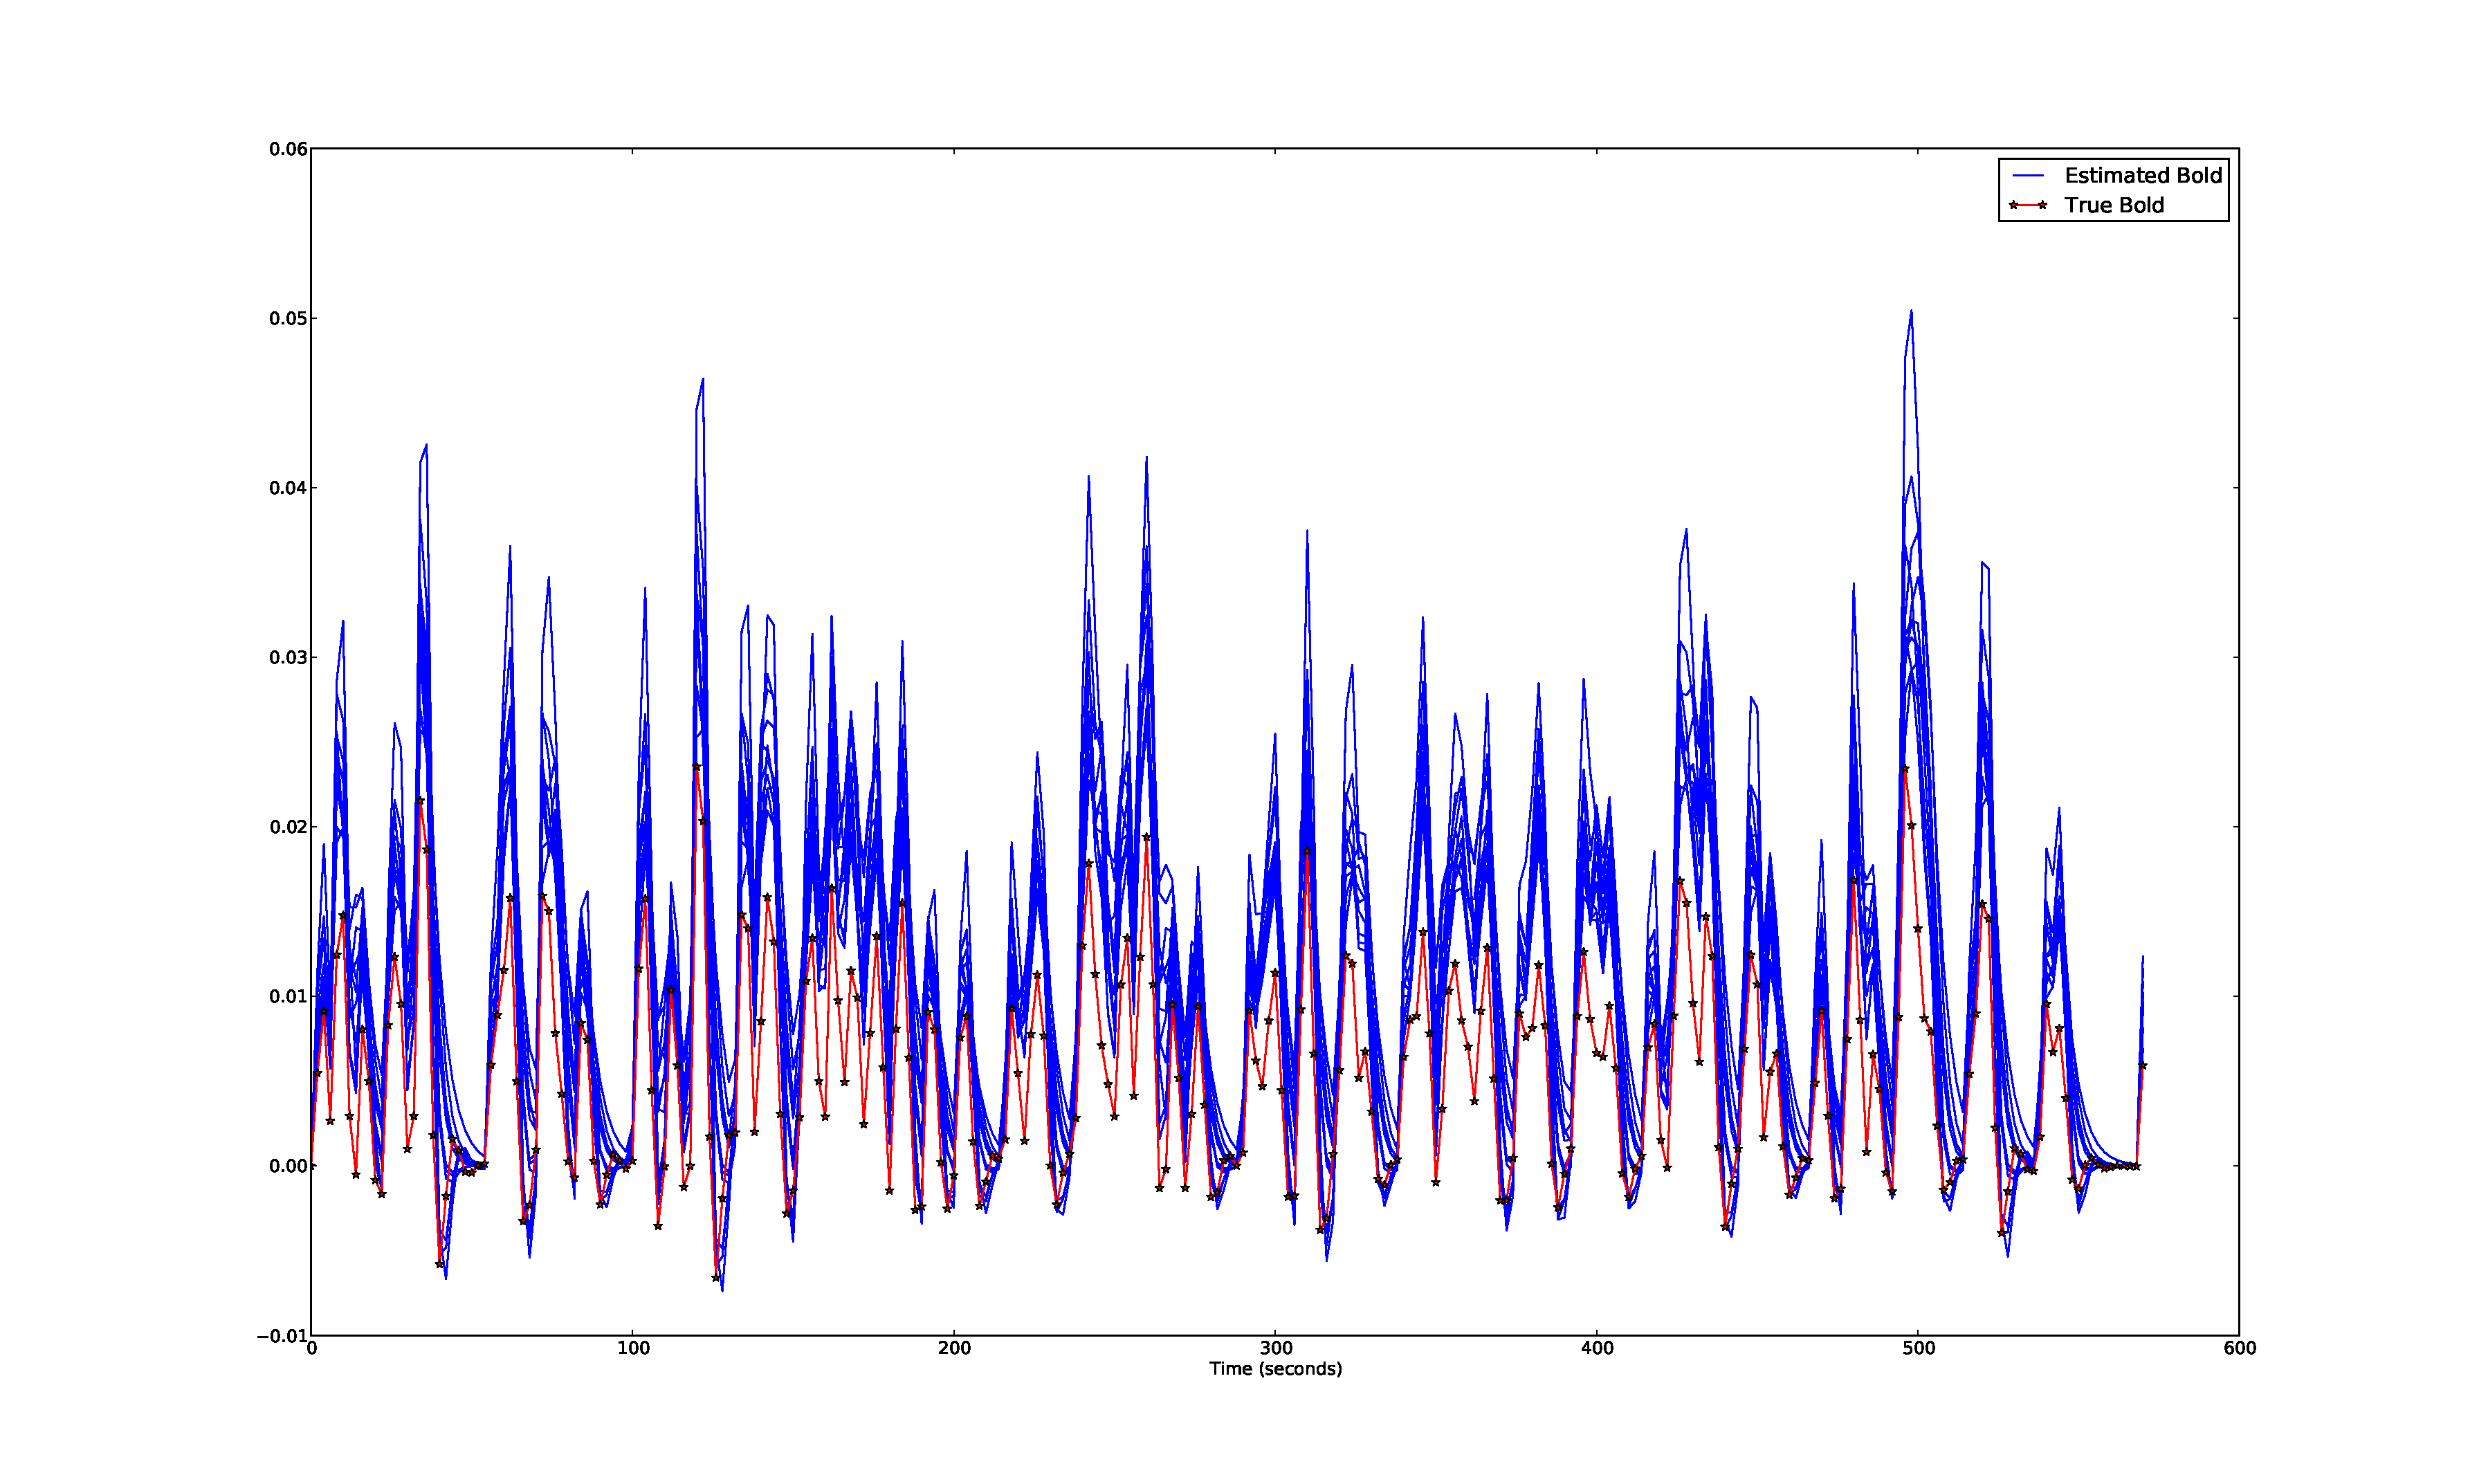
\includegraphics[trim=6cm 3cm 6cm 3cm,width=16cm]{images/comparison_highnoise}
\caption{A comparison of the fitted signals for the high noise case.}
\end{figure}
\begin{figure}[H]
\label{fig:NoiseComparisonJustTwo}
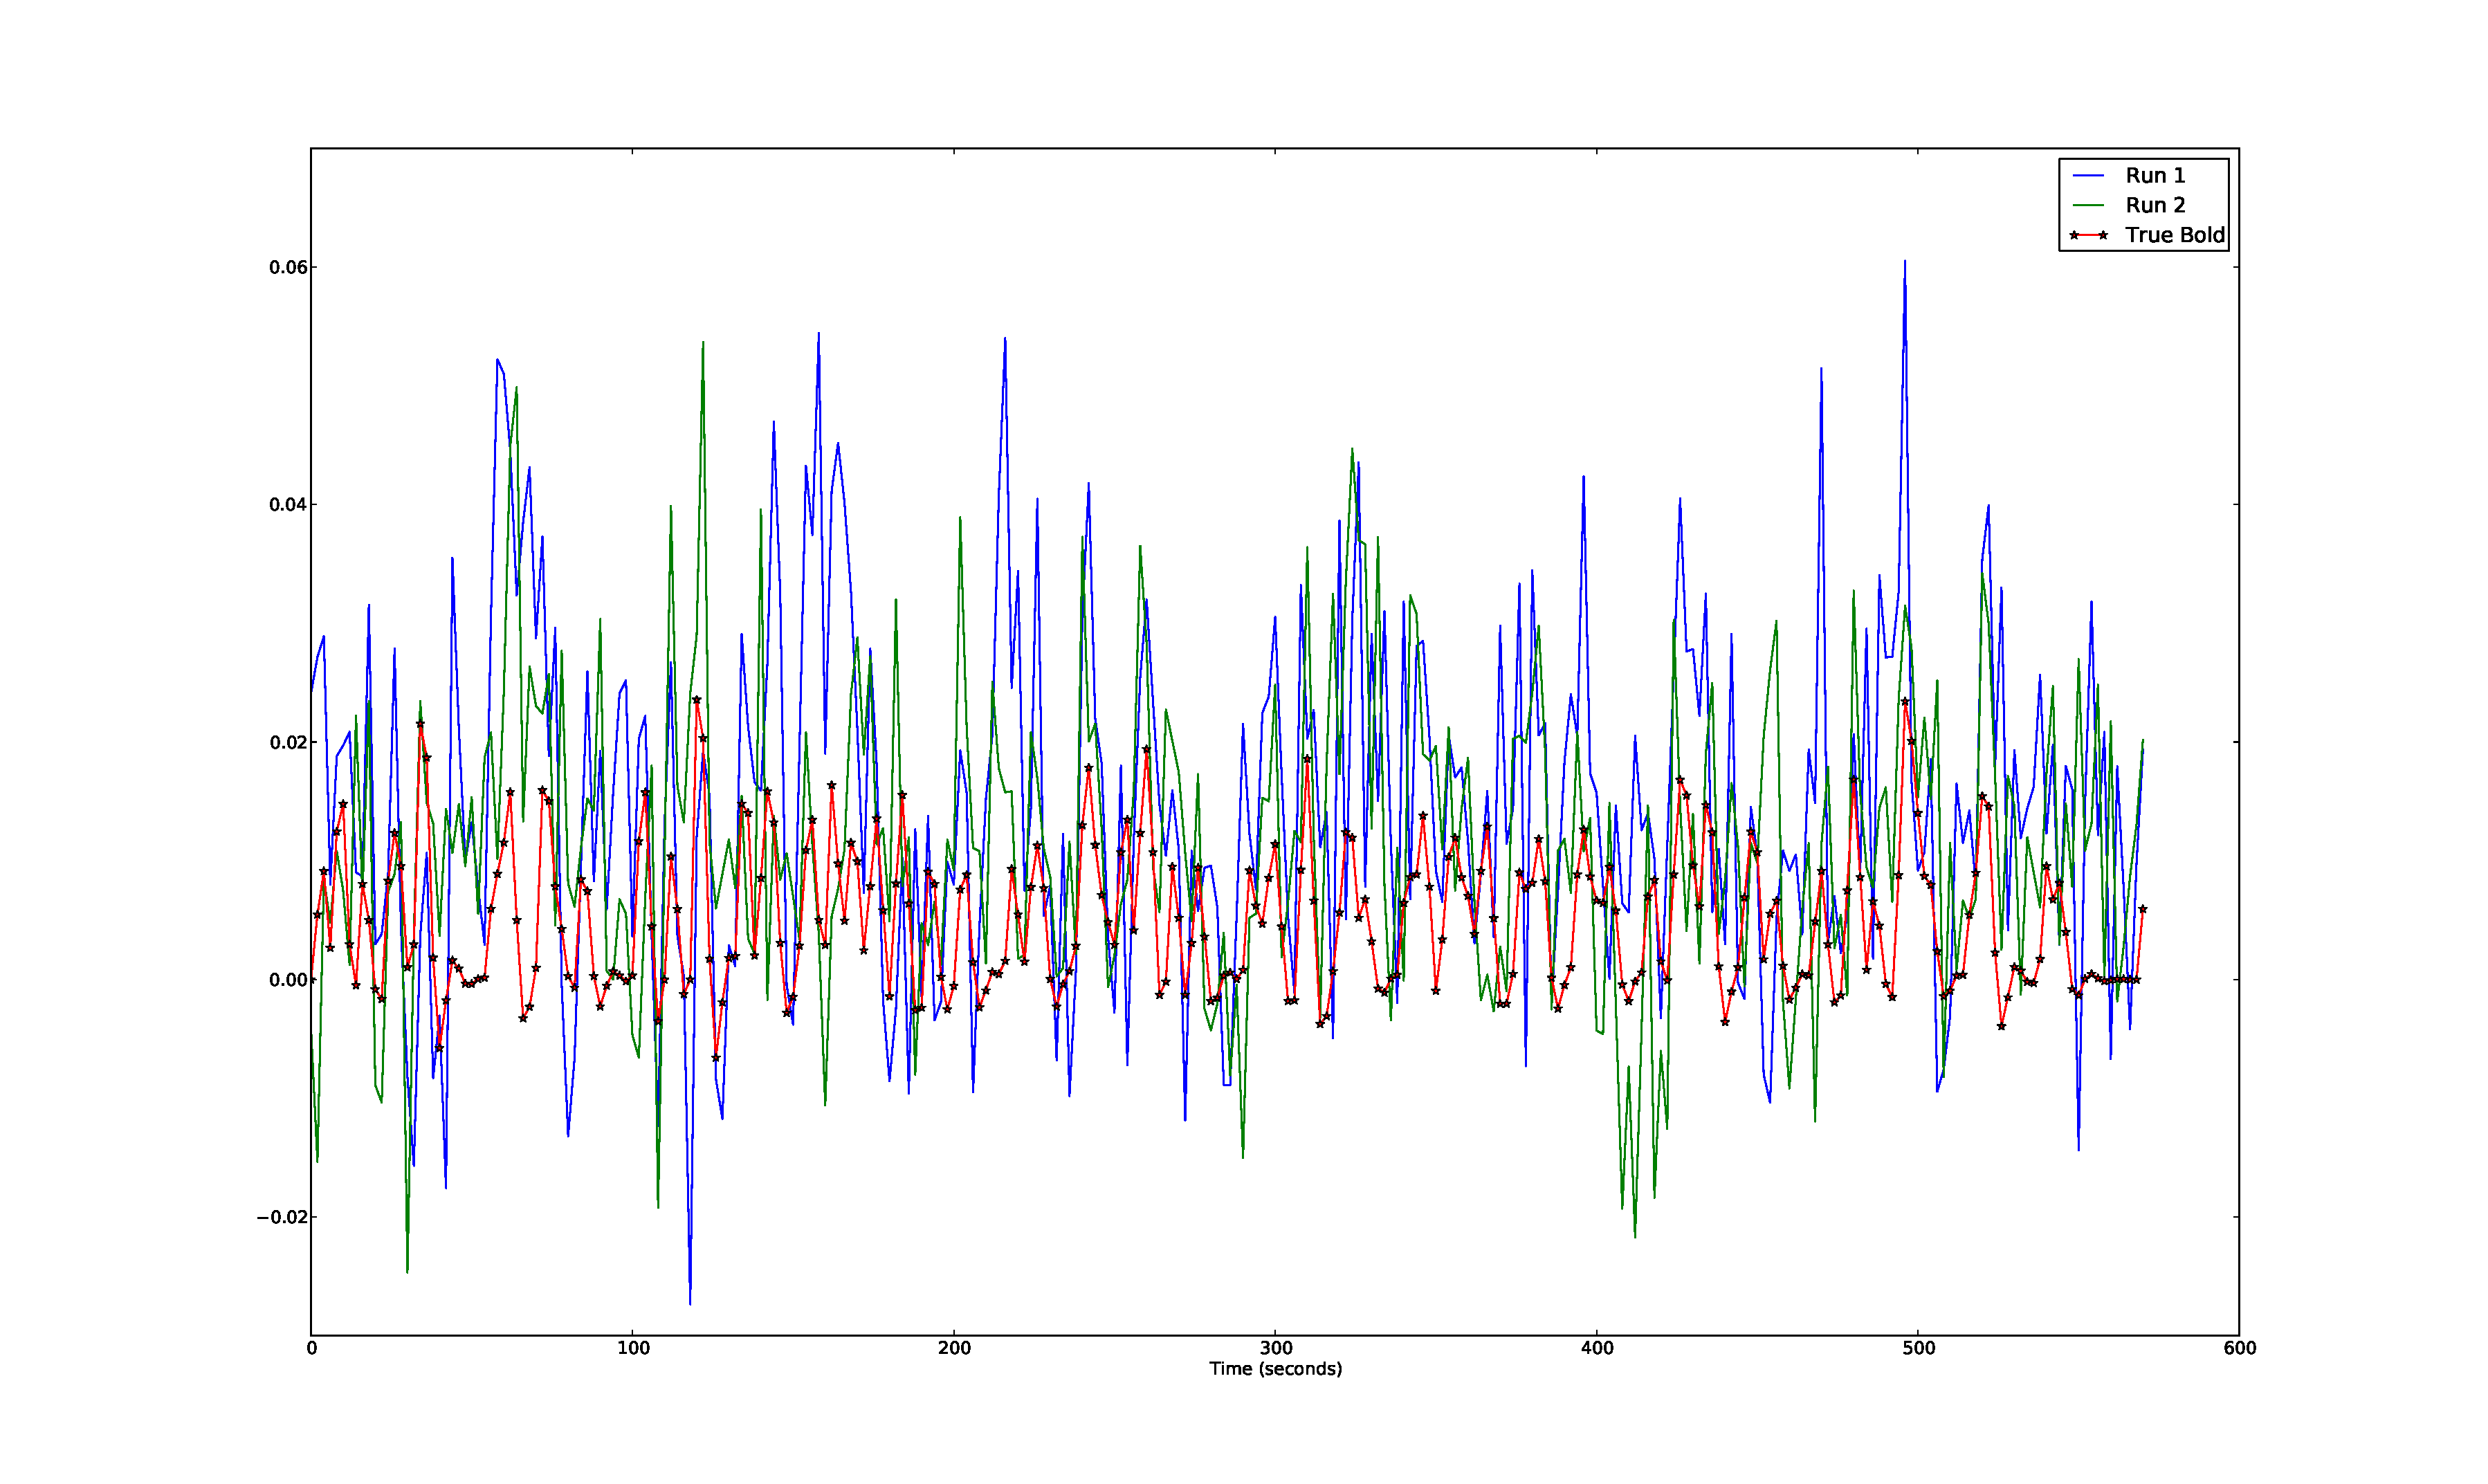
\includegraphics[trim=6cm 3cm 6cm 3cm,width=16cm]{images/highnoise_56_noise}
\caption{Two particular preprocessed noise realizations for the high noise case.}
\end{figure}
\begin{figure}[H]
\label{fig:FitComparisonHighNoiseJust2}
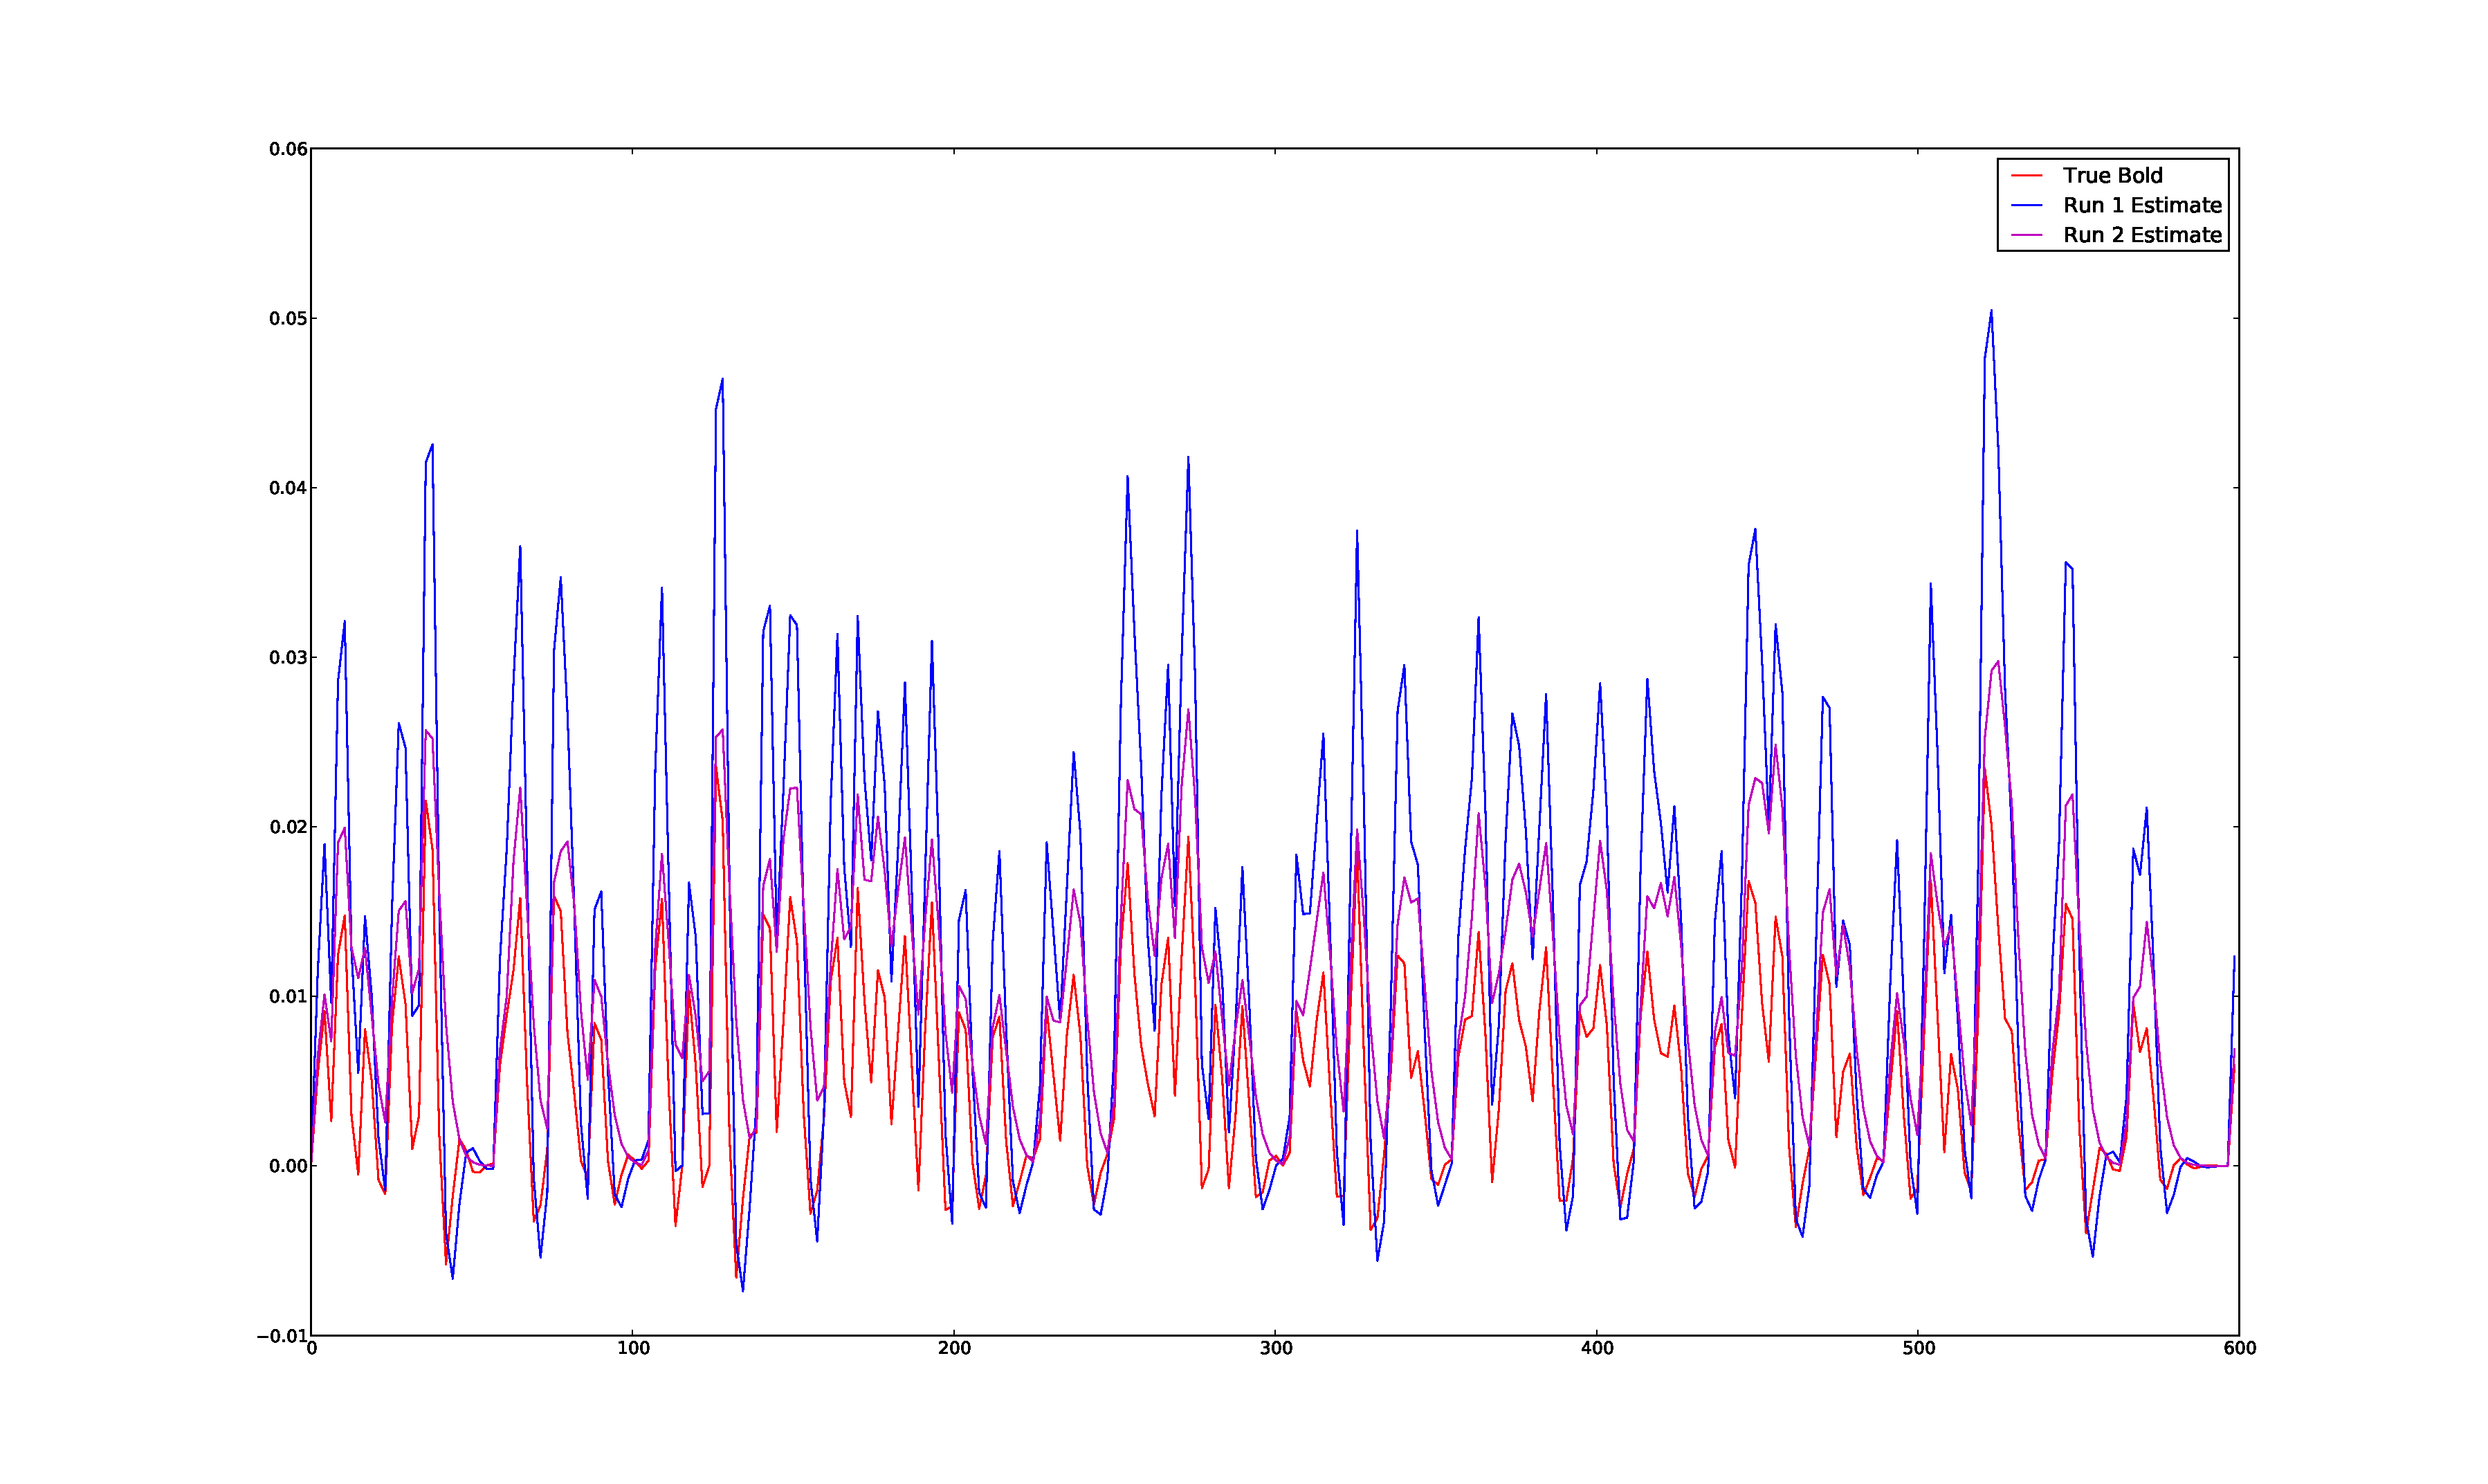
\includegraphics[trim=6cm 3cm 6cm 3cm,width=16cm]{images/comparison_highnoise_just2}
\caption{The results for the noise realizations shown in \autoref{fig:NoiseComparisonJustTwo}.}
\end{figure}

It is interesting to consider how the preprocessing and noise may effect the
parameters of the fitting model. For instance run 1 in \autoref{fig:NoiseComparisonJustTwo}
certainly seems to be more biased toward higher peaks than run 2. There also appears
to be more drift than the 20 points per knot could fit, which explains the 
prolonged increase at 170 seconds. Despite run 1's bias toward higher peaks, for
some reason the particle filter was able to get a much better match for the
modeled post-stimulus undershoot (which is likely significantly shorter than it
should be). Ultimately the results are pretty good. \autoref{tab:SimMSE} shows
the mean squared error for all two runs, and highlights the two runs analyzed here and 
in \autoref{fig:ConvergenceRuns1} and \autoref{fig:ConvergenceRuns2}.

\begin{figure}[H]
\subfigure[$\tau_0$, $\alpha$, $E_0$, $V_0$]
{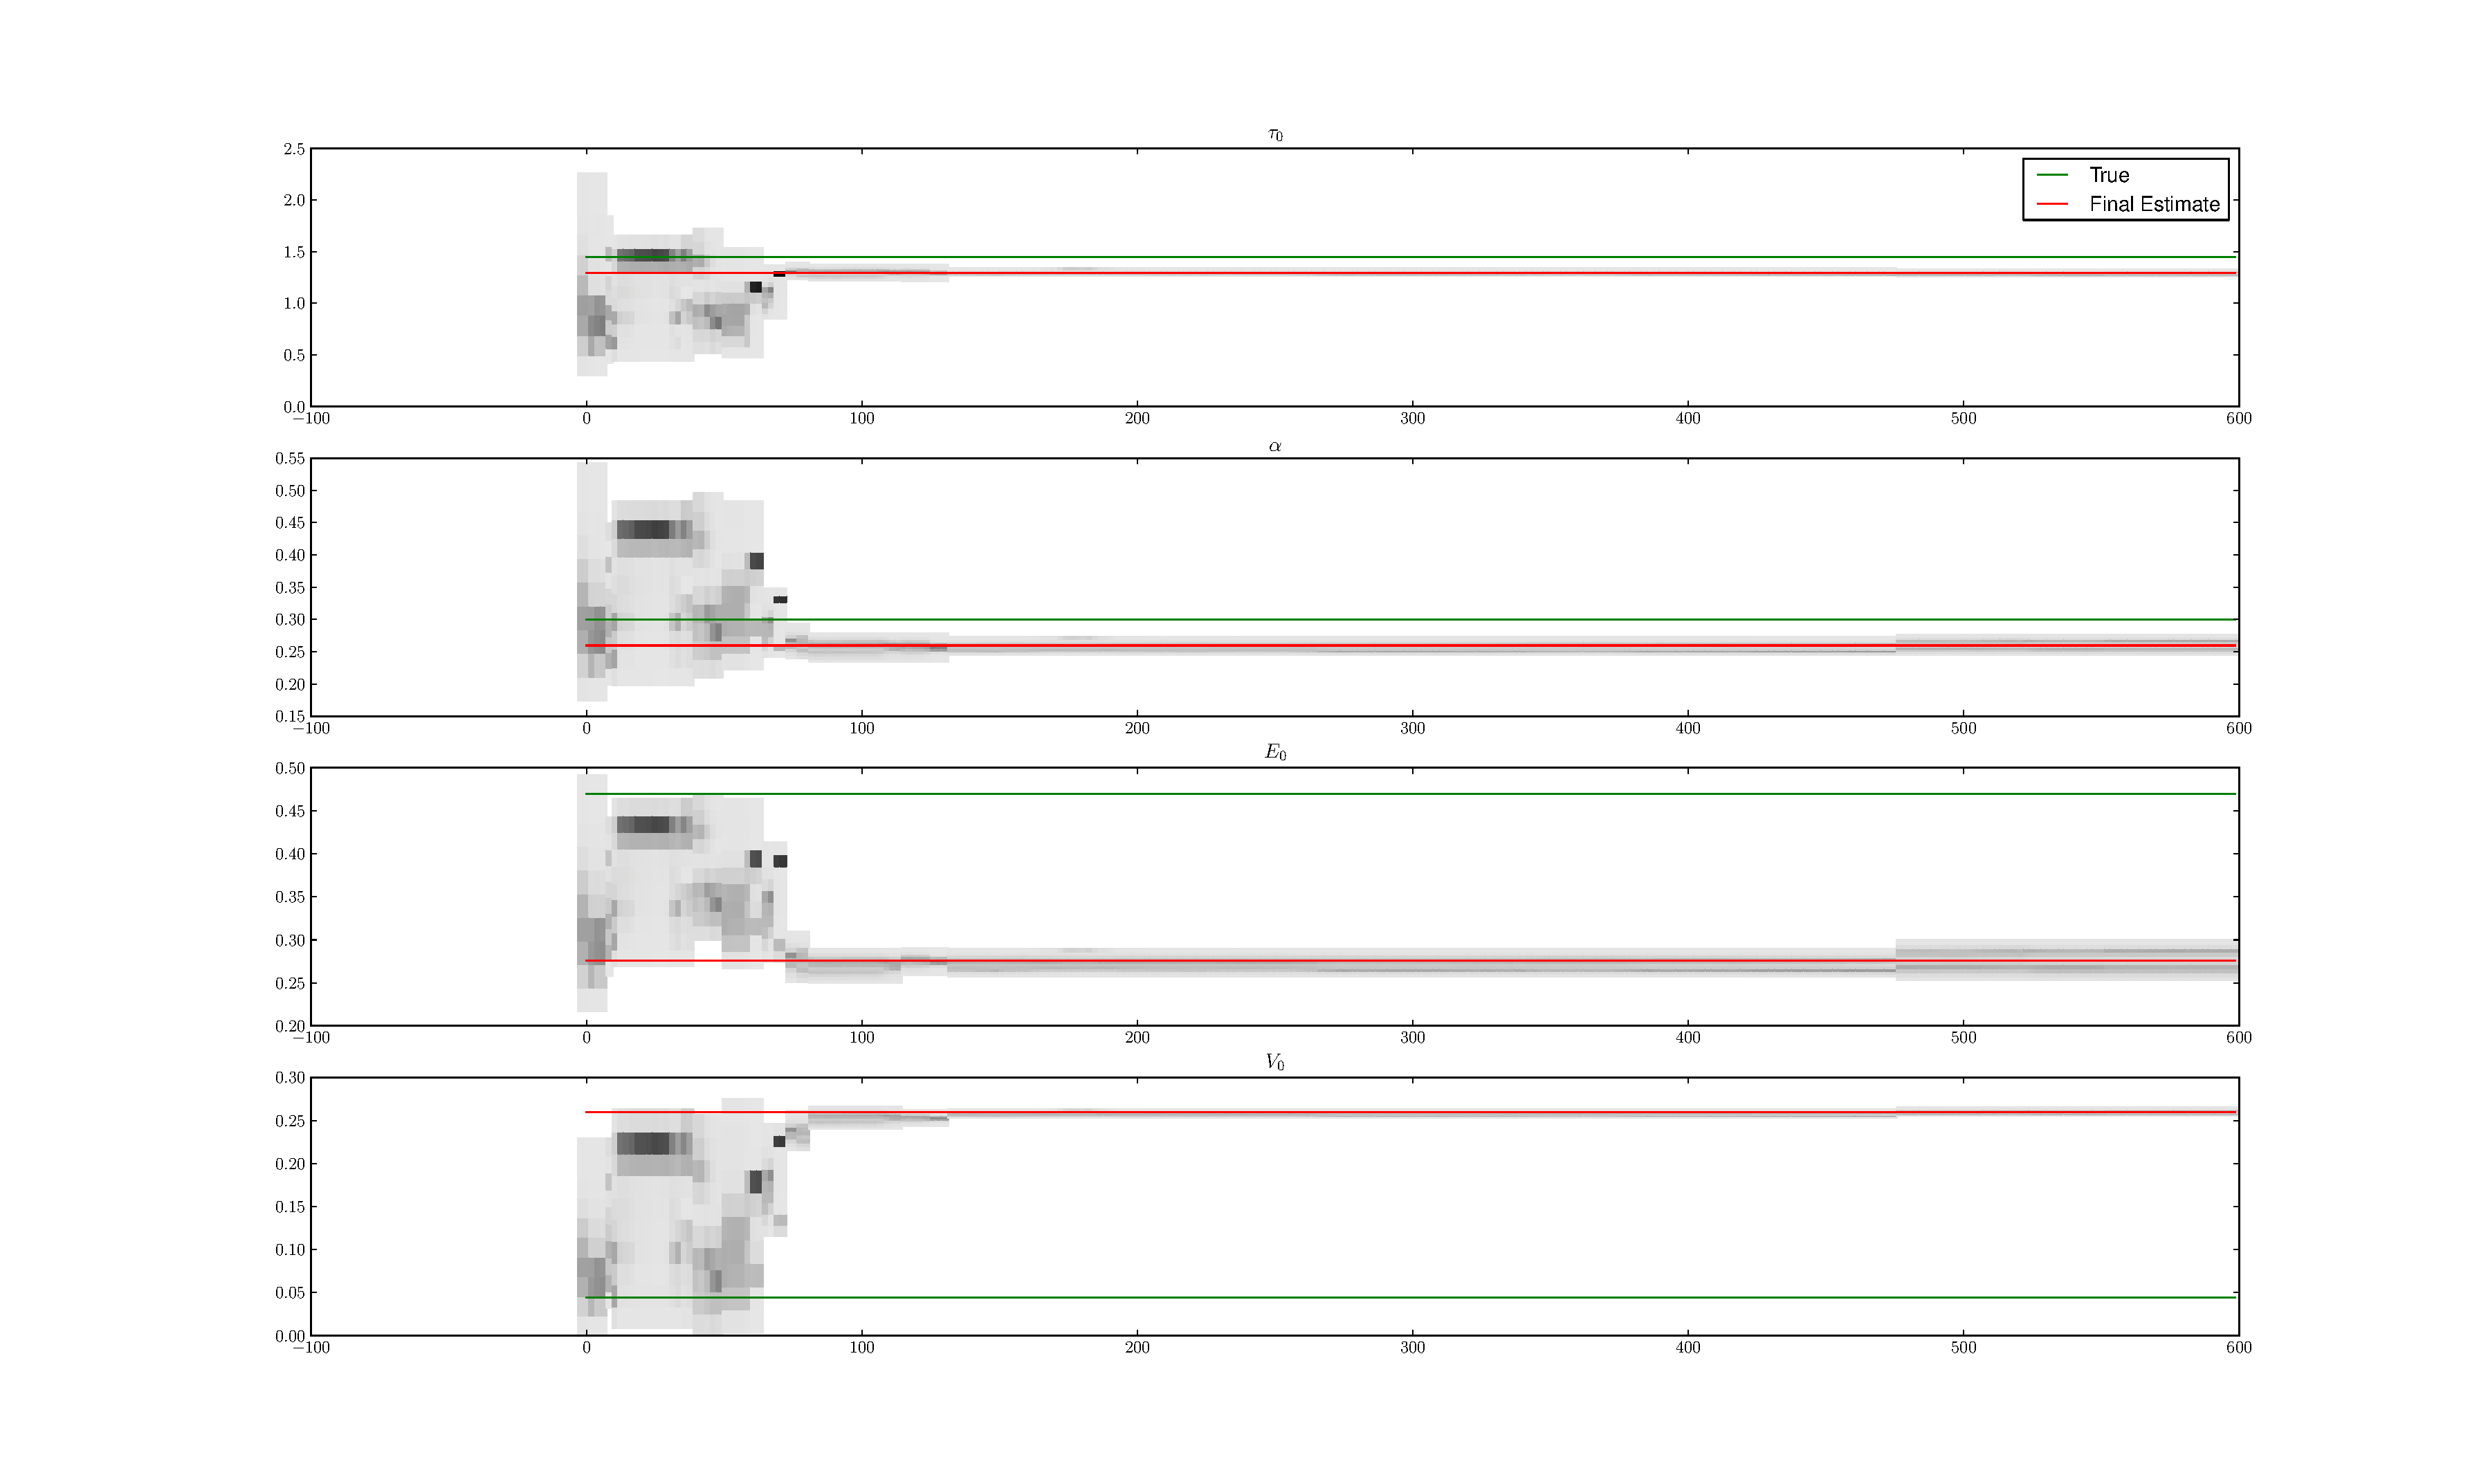
\includegraphics[trim=7cm 3cm 7cm 4cm, width=15cm]{images/highnoise_run5_1}}\\
\end{figure}
\begin{figure}[H]
\subfigure[$\tau_s$, $\tau_f$, $\epsilon$, $V$] 
{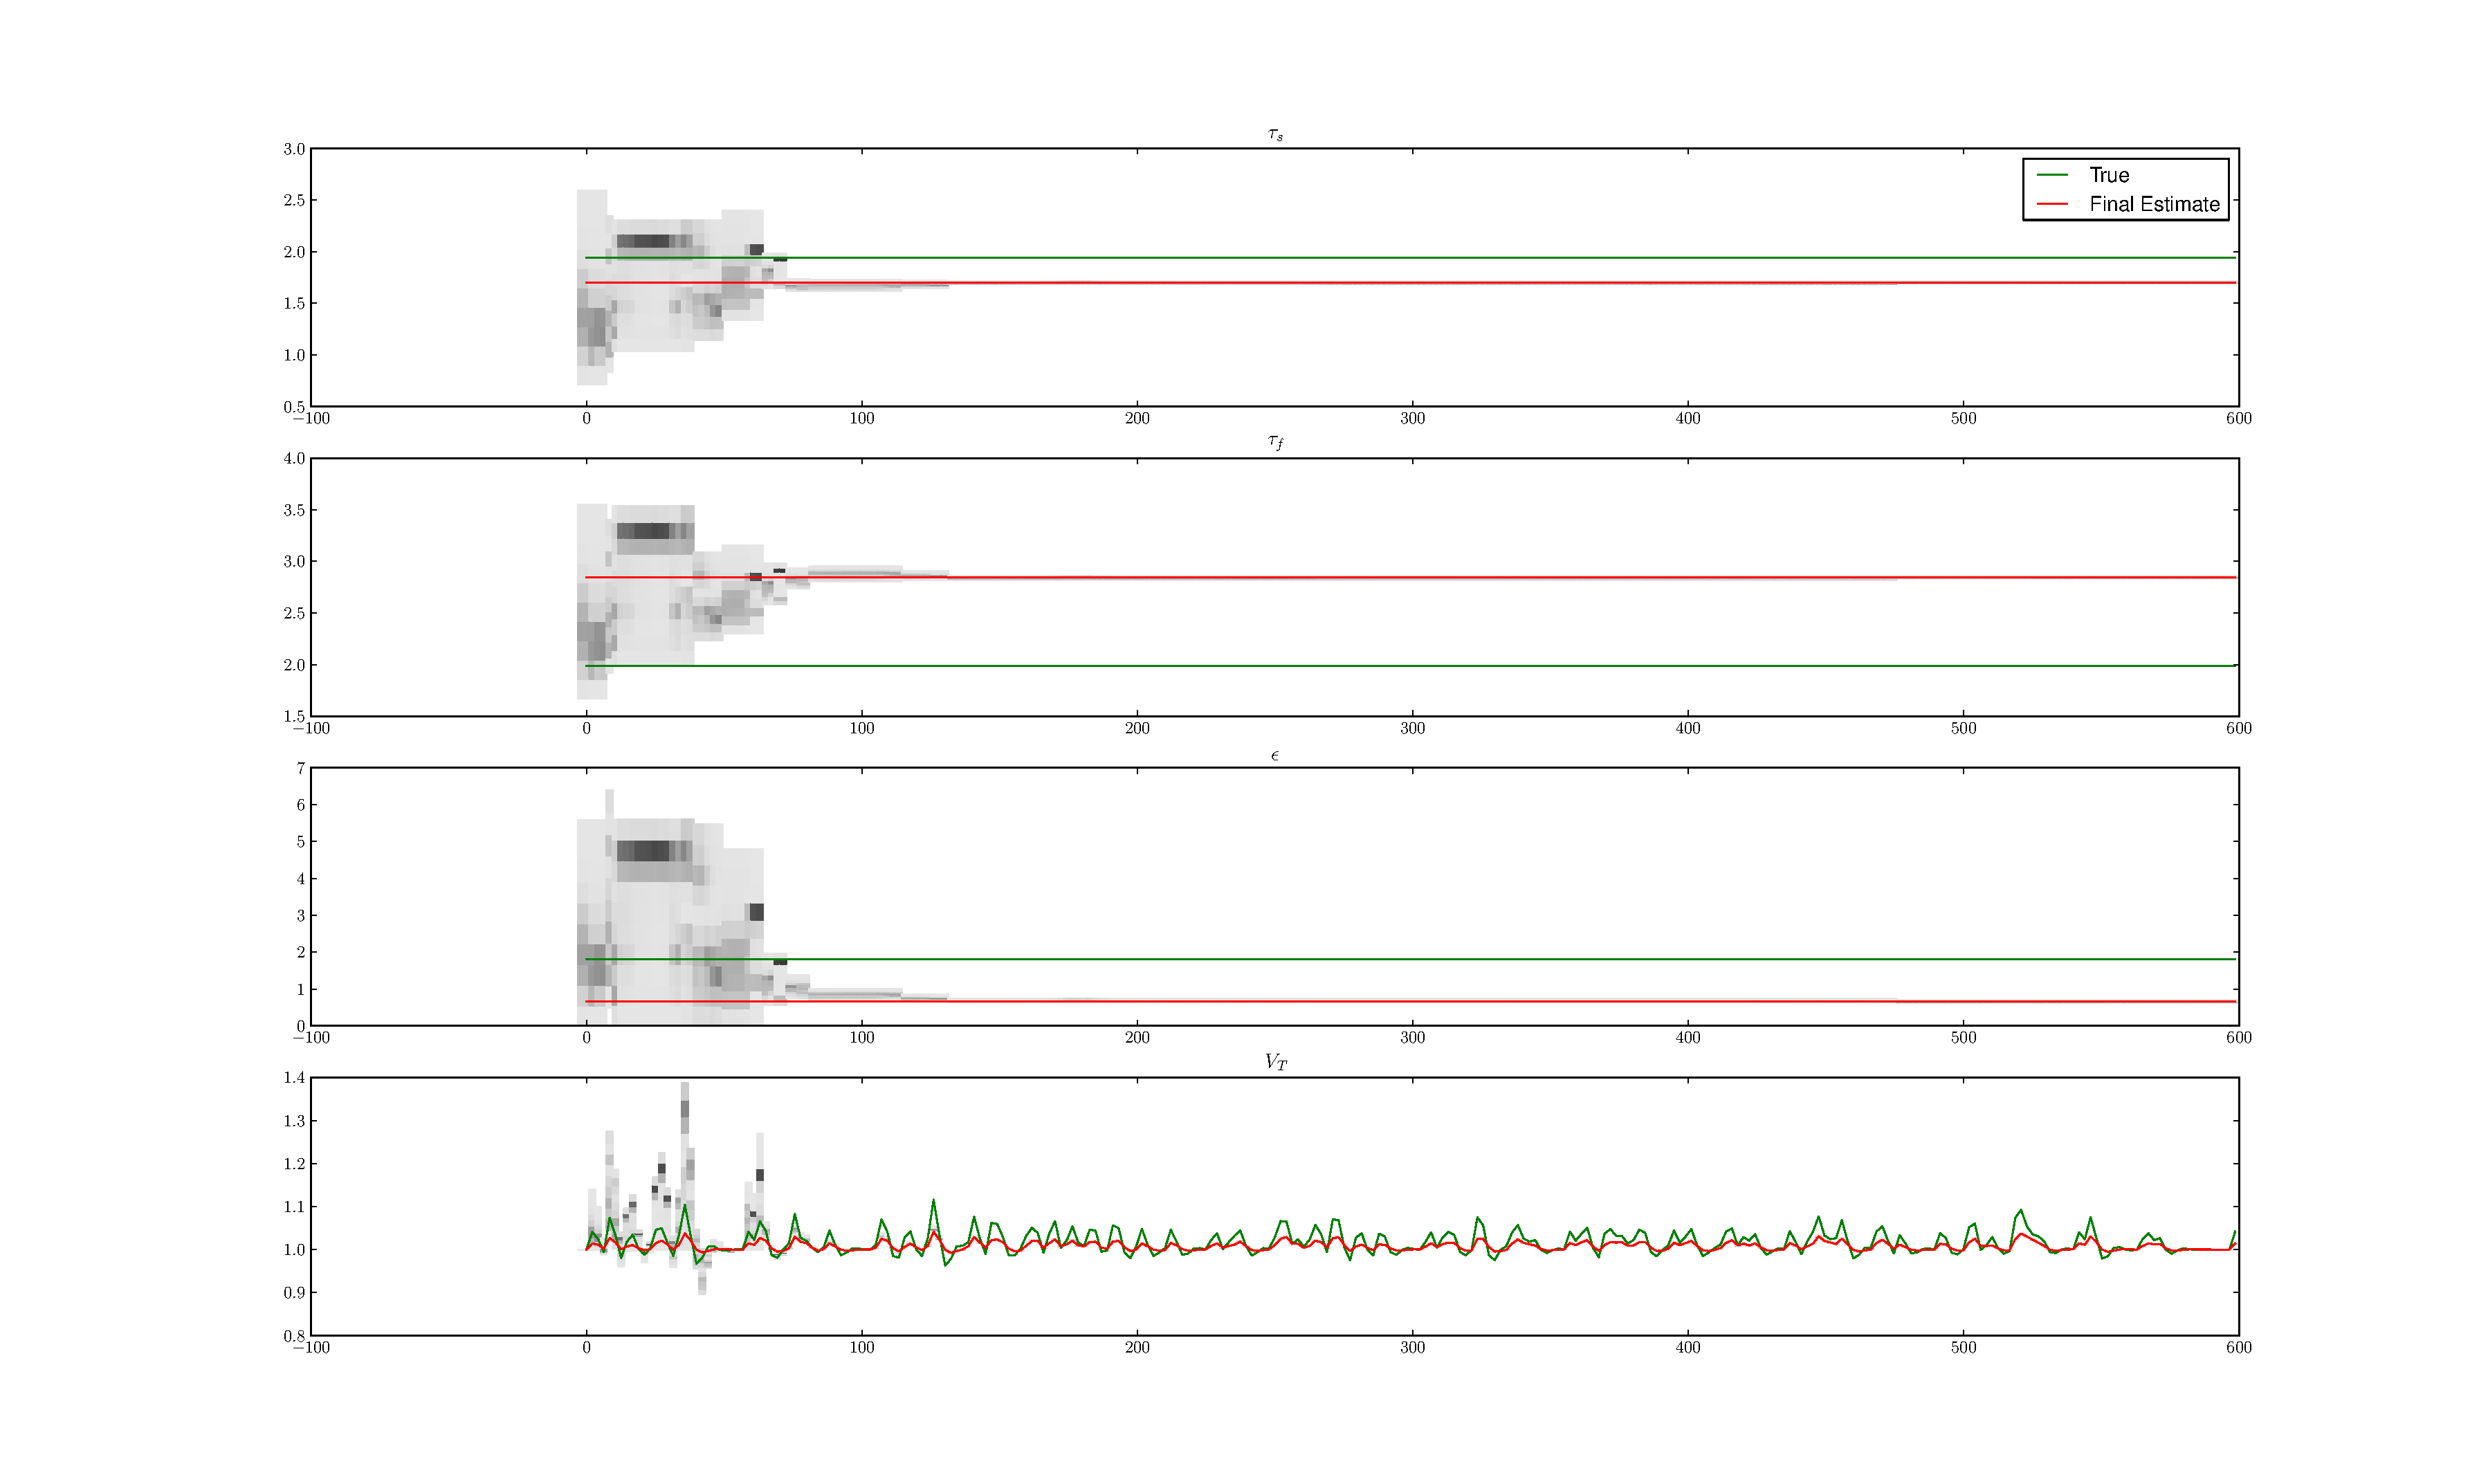
\includegraphics[trim=7cm 3cm 7cm 1cm, width=15cm]{images/highnoise_run5_2}}\\
\end{figure}
\begin{figure}[H]
\subfigure[$Q$, $S$, $F$, $BOLD$ ]
{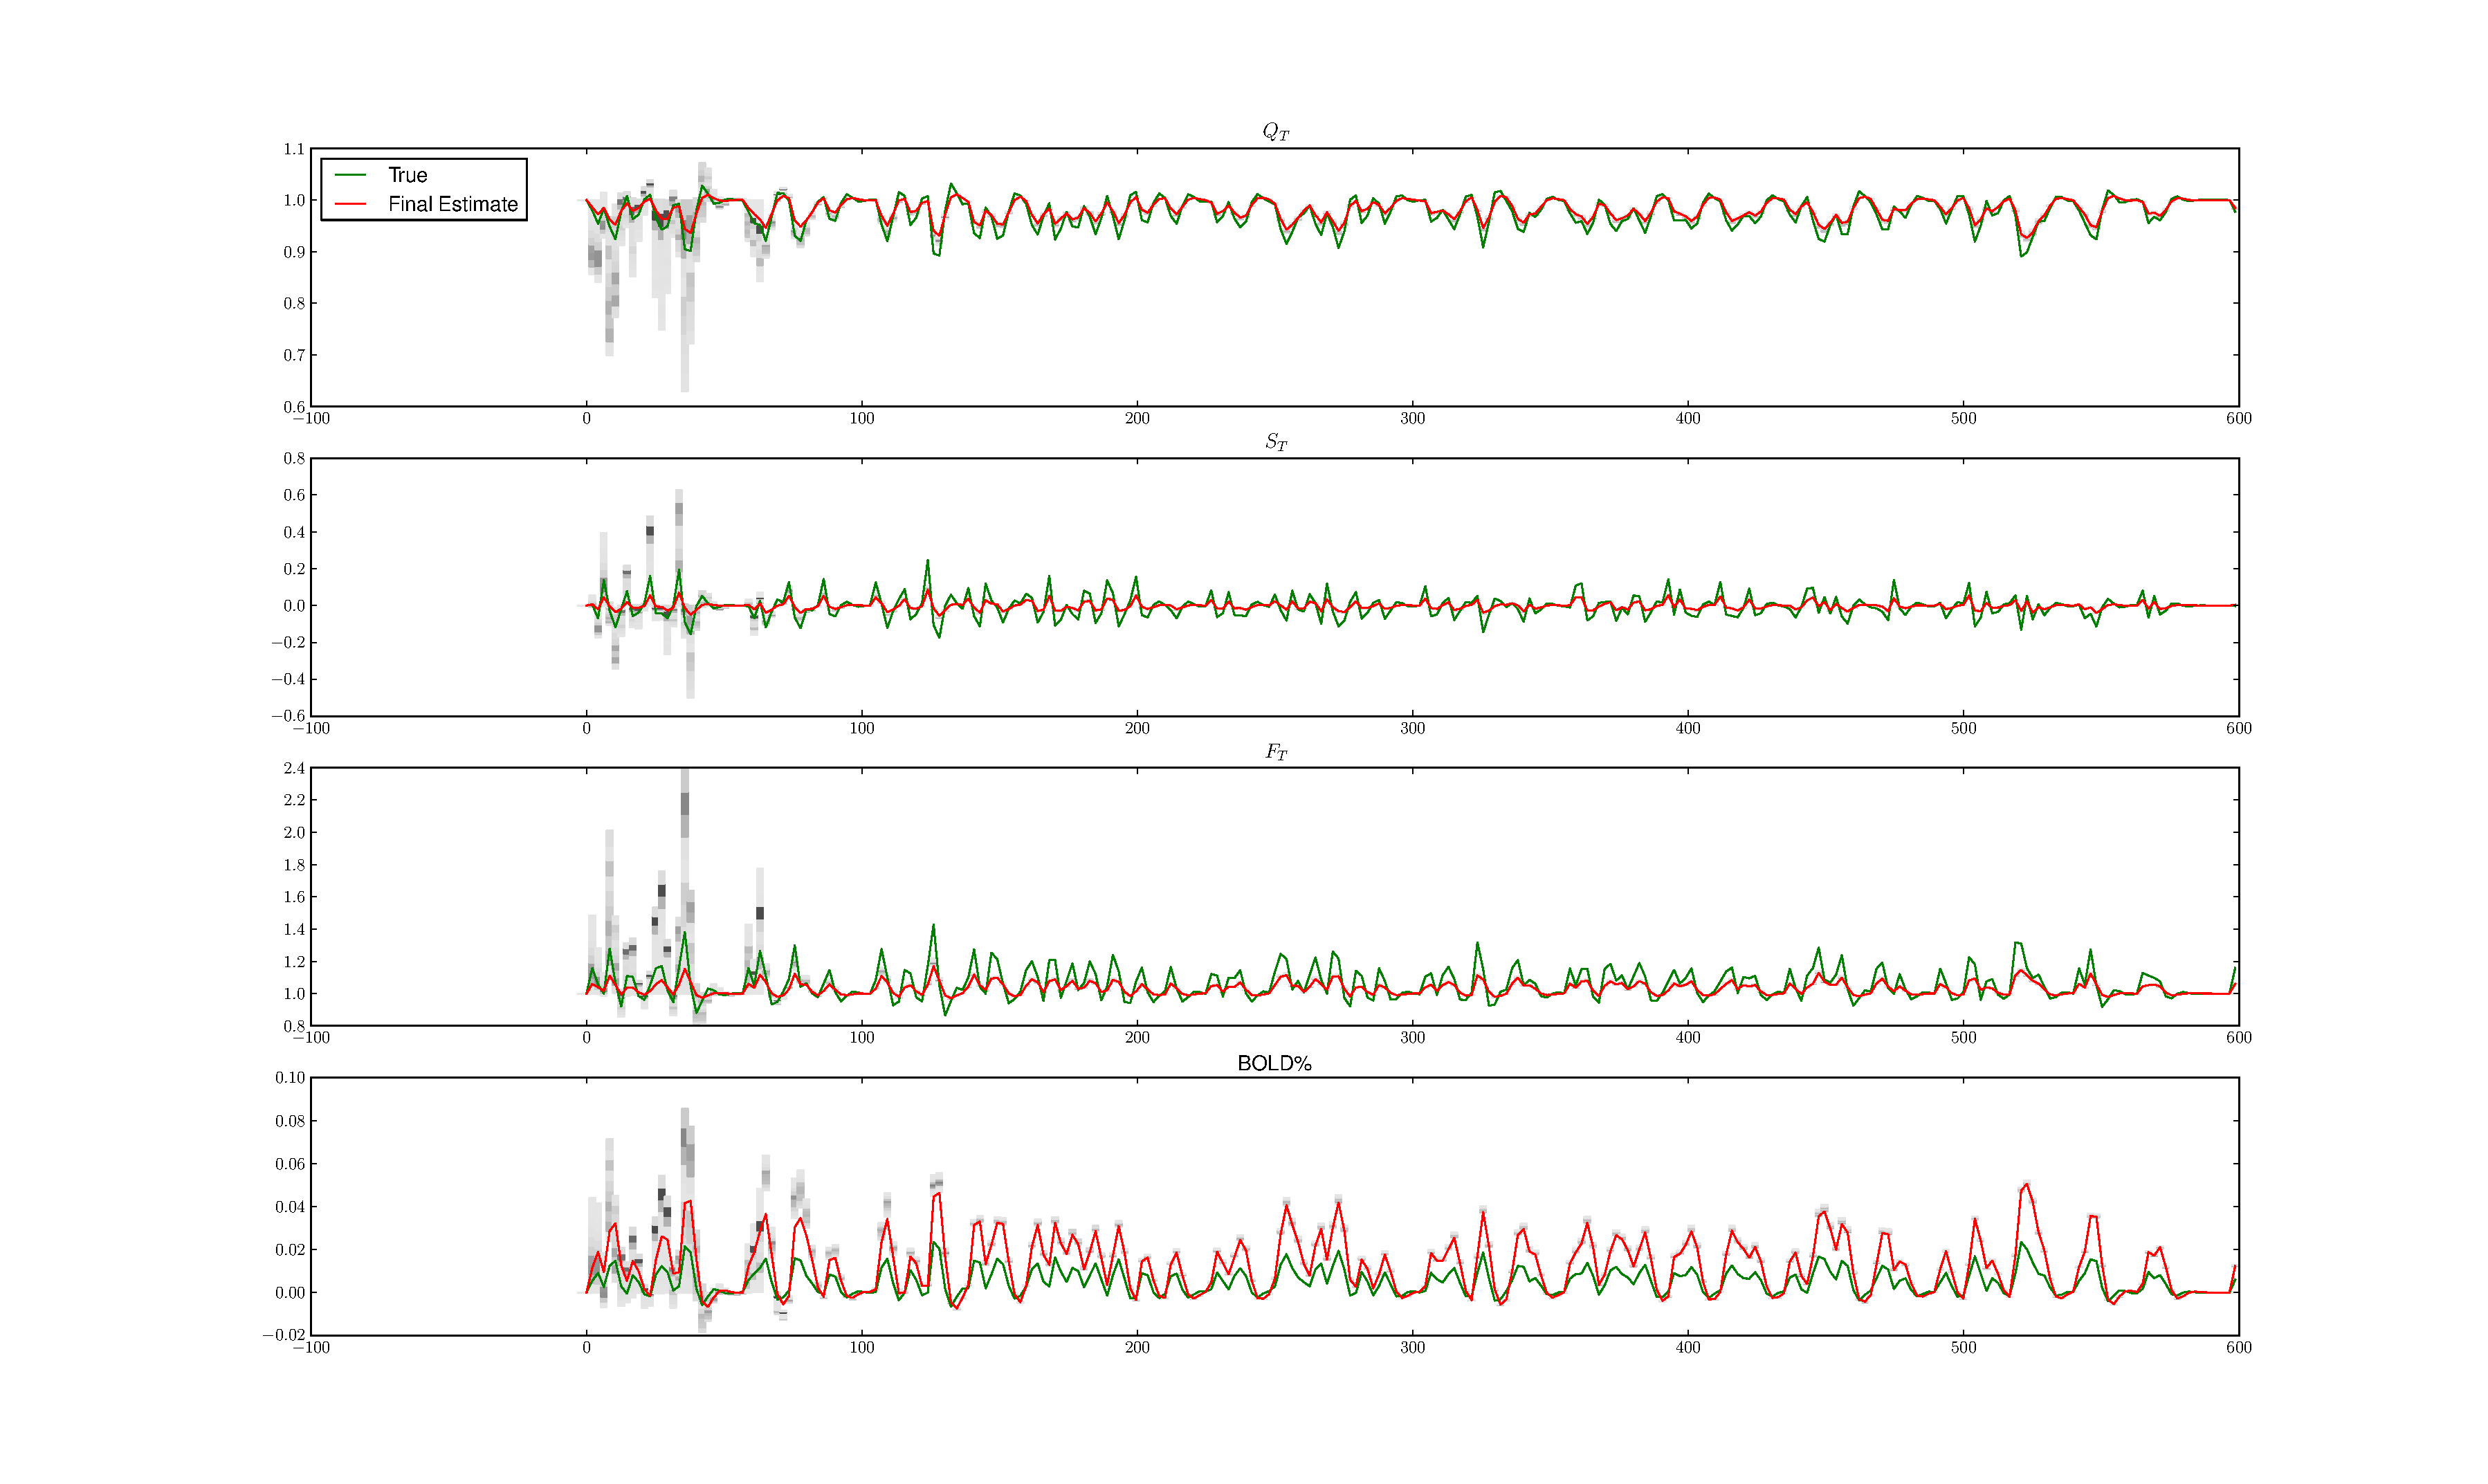
\includegraphics[trim=7cm 3cm 7cm 2cm, width=15cm]{images/highnoise_run5_3}}
\label{fig:ConvergenceRuns1}
\caption{Converging histogram for parameters during run 1, as in \autoref{fig:NoiseComparisonJustTwo}.}
\end{figure}

There are a number of interesting convergence properties of the
particle filter when more noise is present, as both \autoref{fig:ConvergenceRuns1} and
\autoref{fig:ConvergenceRuns2} show. Obviously the particle filter seems to converge
significantly faster, as points tend to be further out on the weighting function. This
also causes significantly more resampling which is the explanation for the seeming
jumps in resolution that occur from time to time. 

\begin{figure}[H]
\subfigure[$\tau_0$, $\alpha$, $E_0$, $V_0$]
{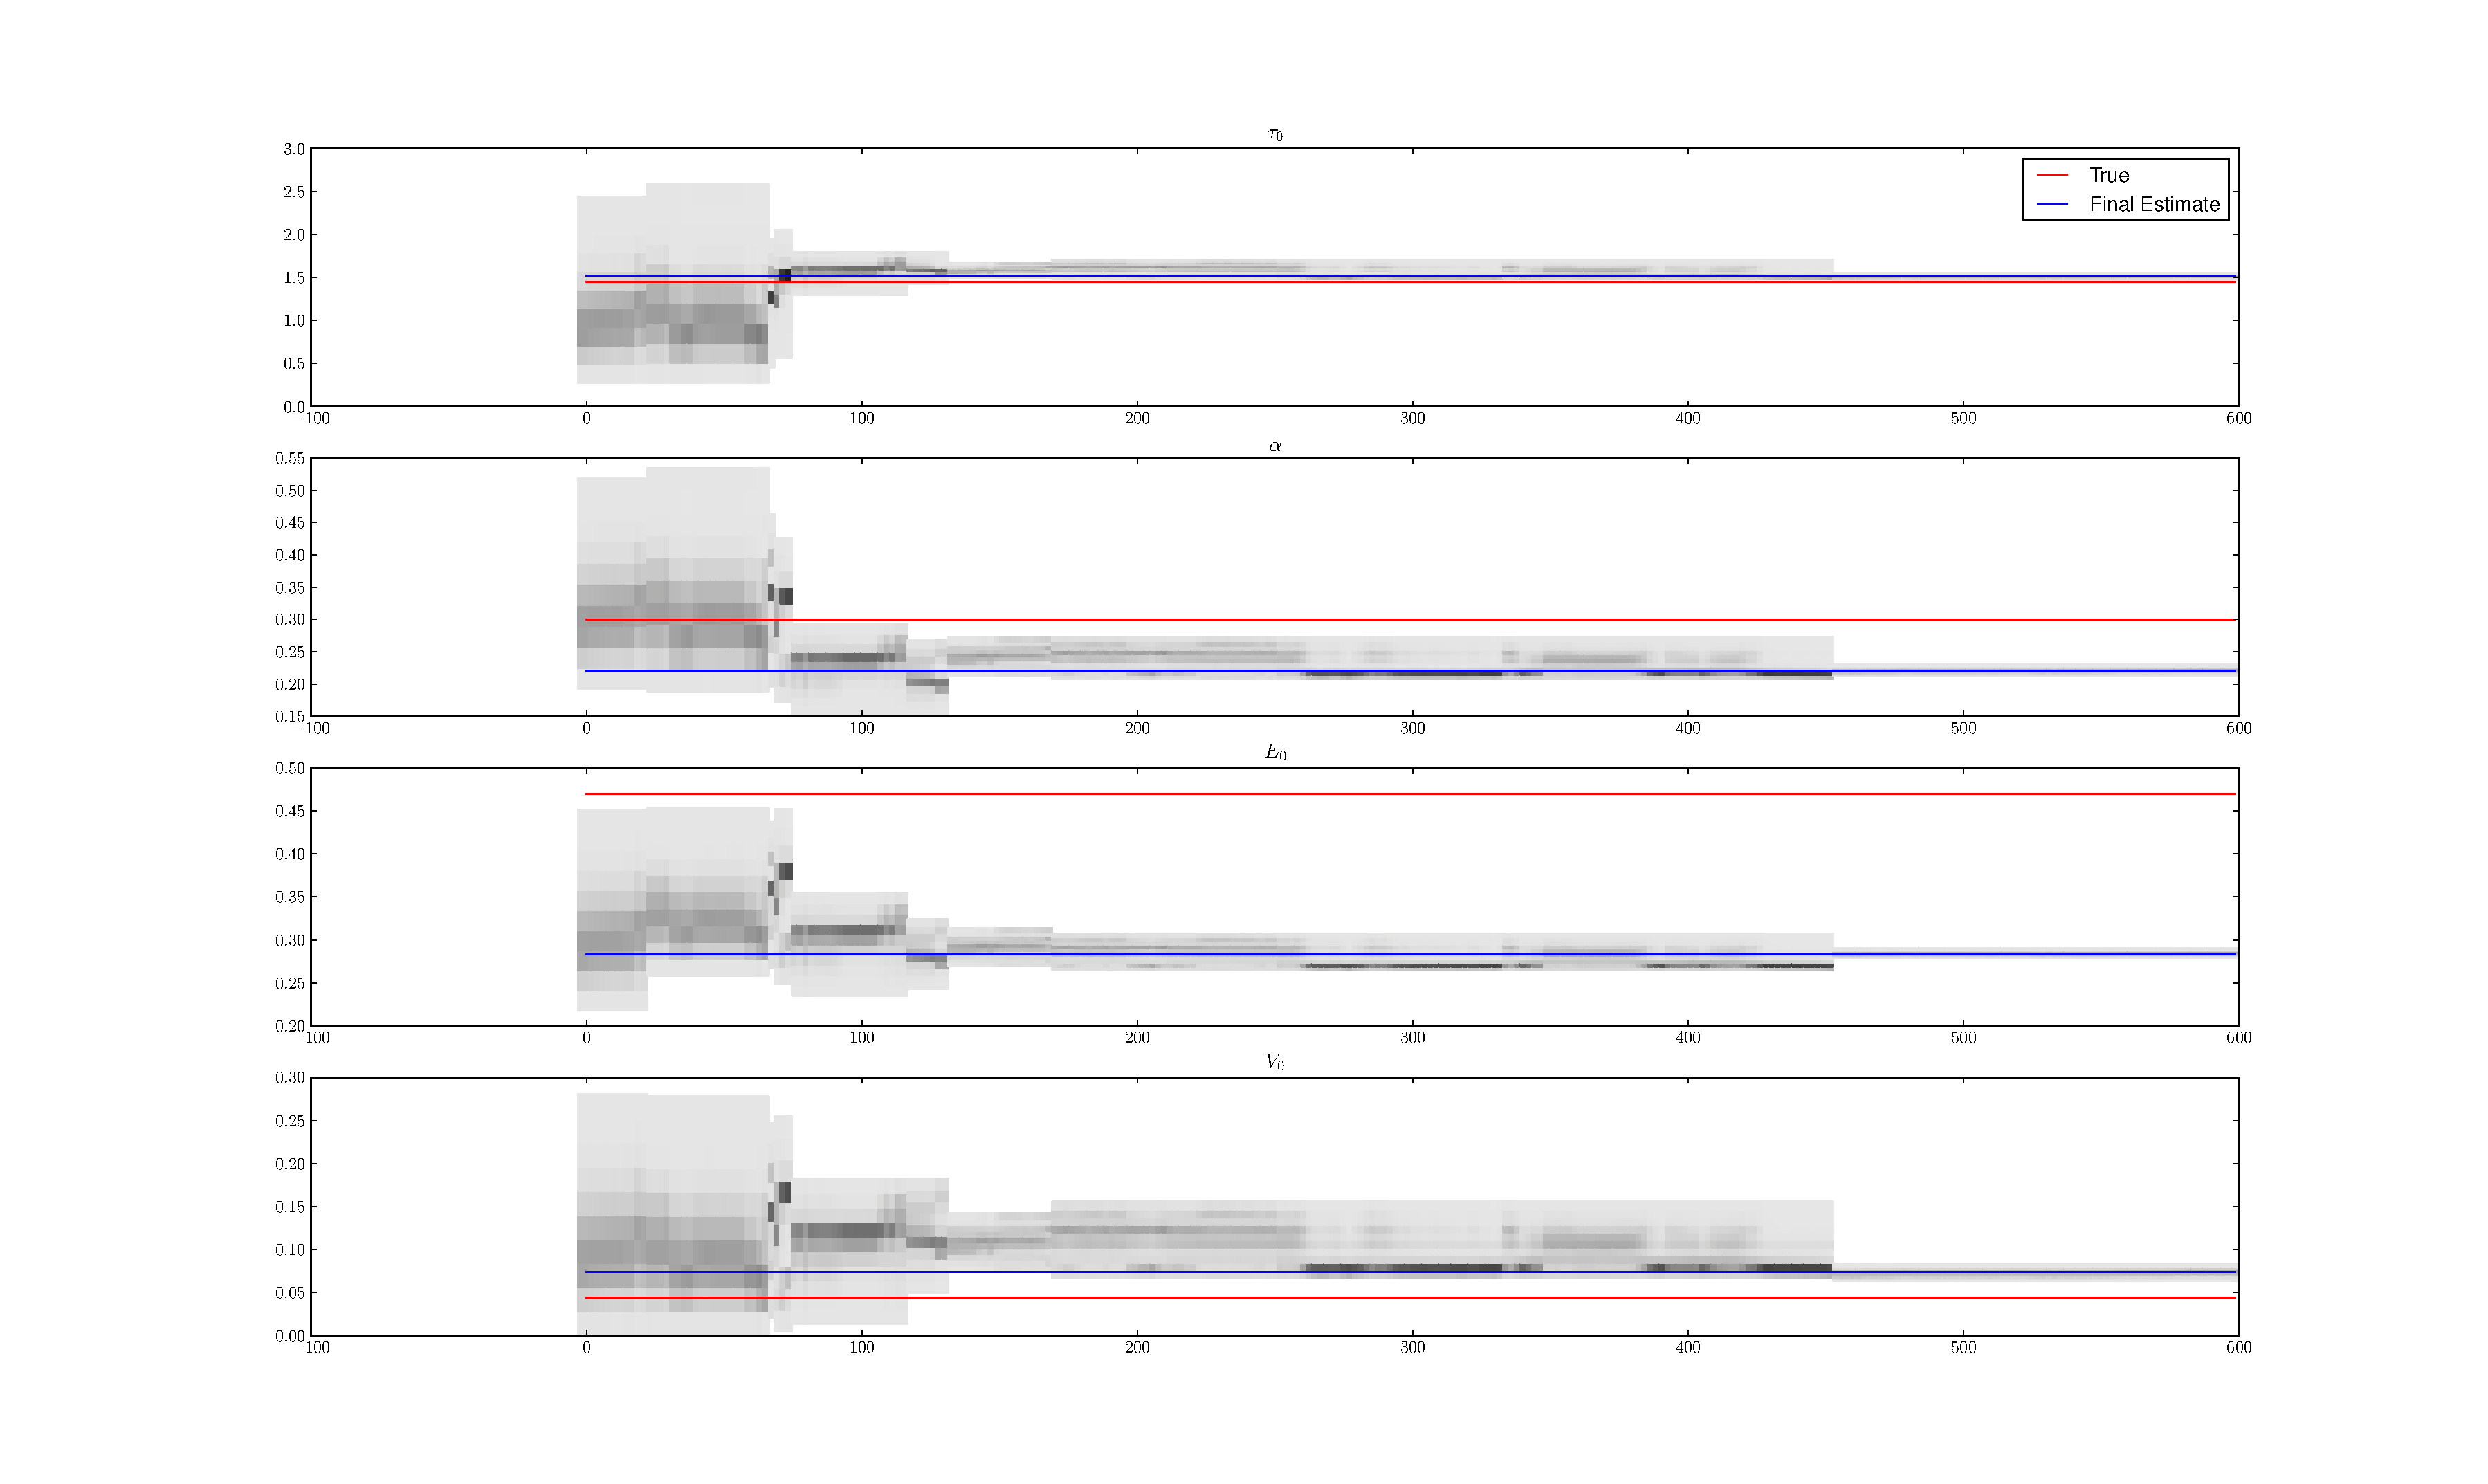
\includegraphics[trim=7cm 3cm 7cm 4cm, width=15cm]{images/highnoise_run6_1}}\\
\end{figure}
\begin{figure}[H]
\subfigure[$\tau_s$, $\tau_f$, $\epsilon$, $V$] 
{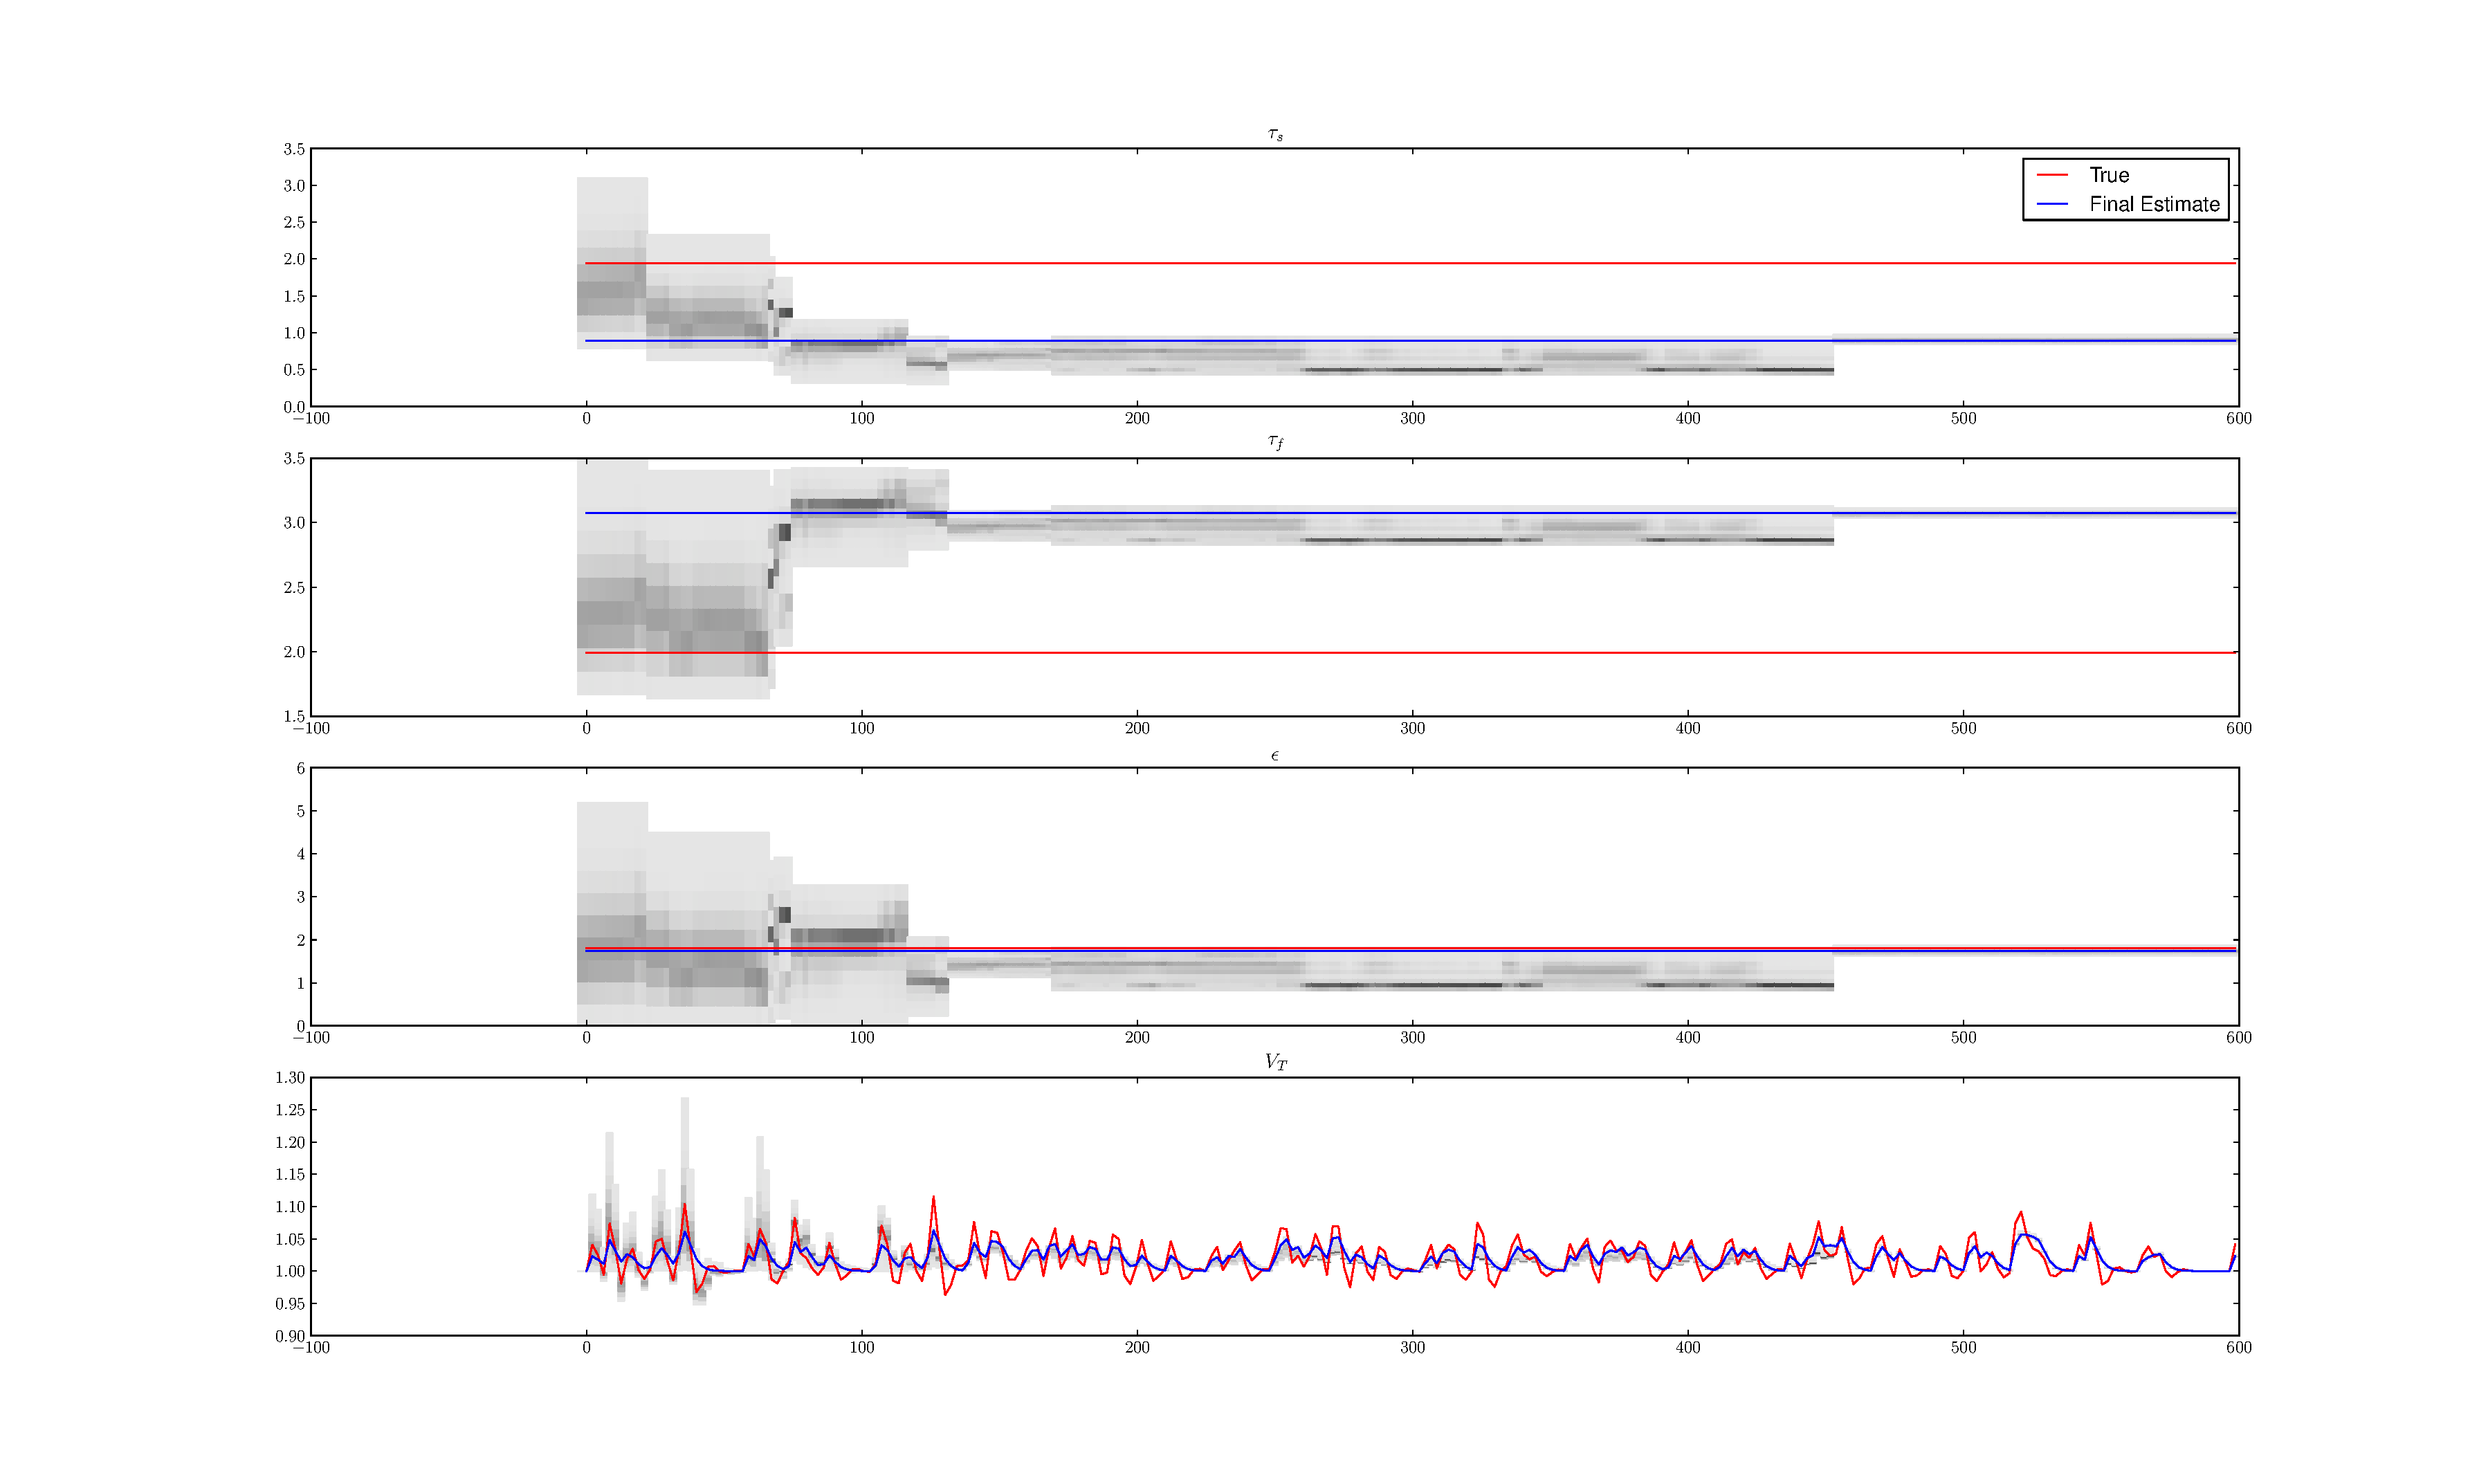
\includegraphics[trim=7cm 3cm 7cm 1cm, width=15cm]{images/highnoise_run6_2}}\\
\end{figure}
\begin{figure}[H]
\subfigure[$Q$, $S$, $F$, $BOLD$ ]
{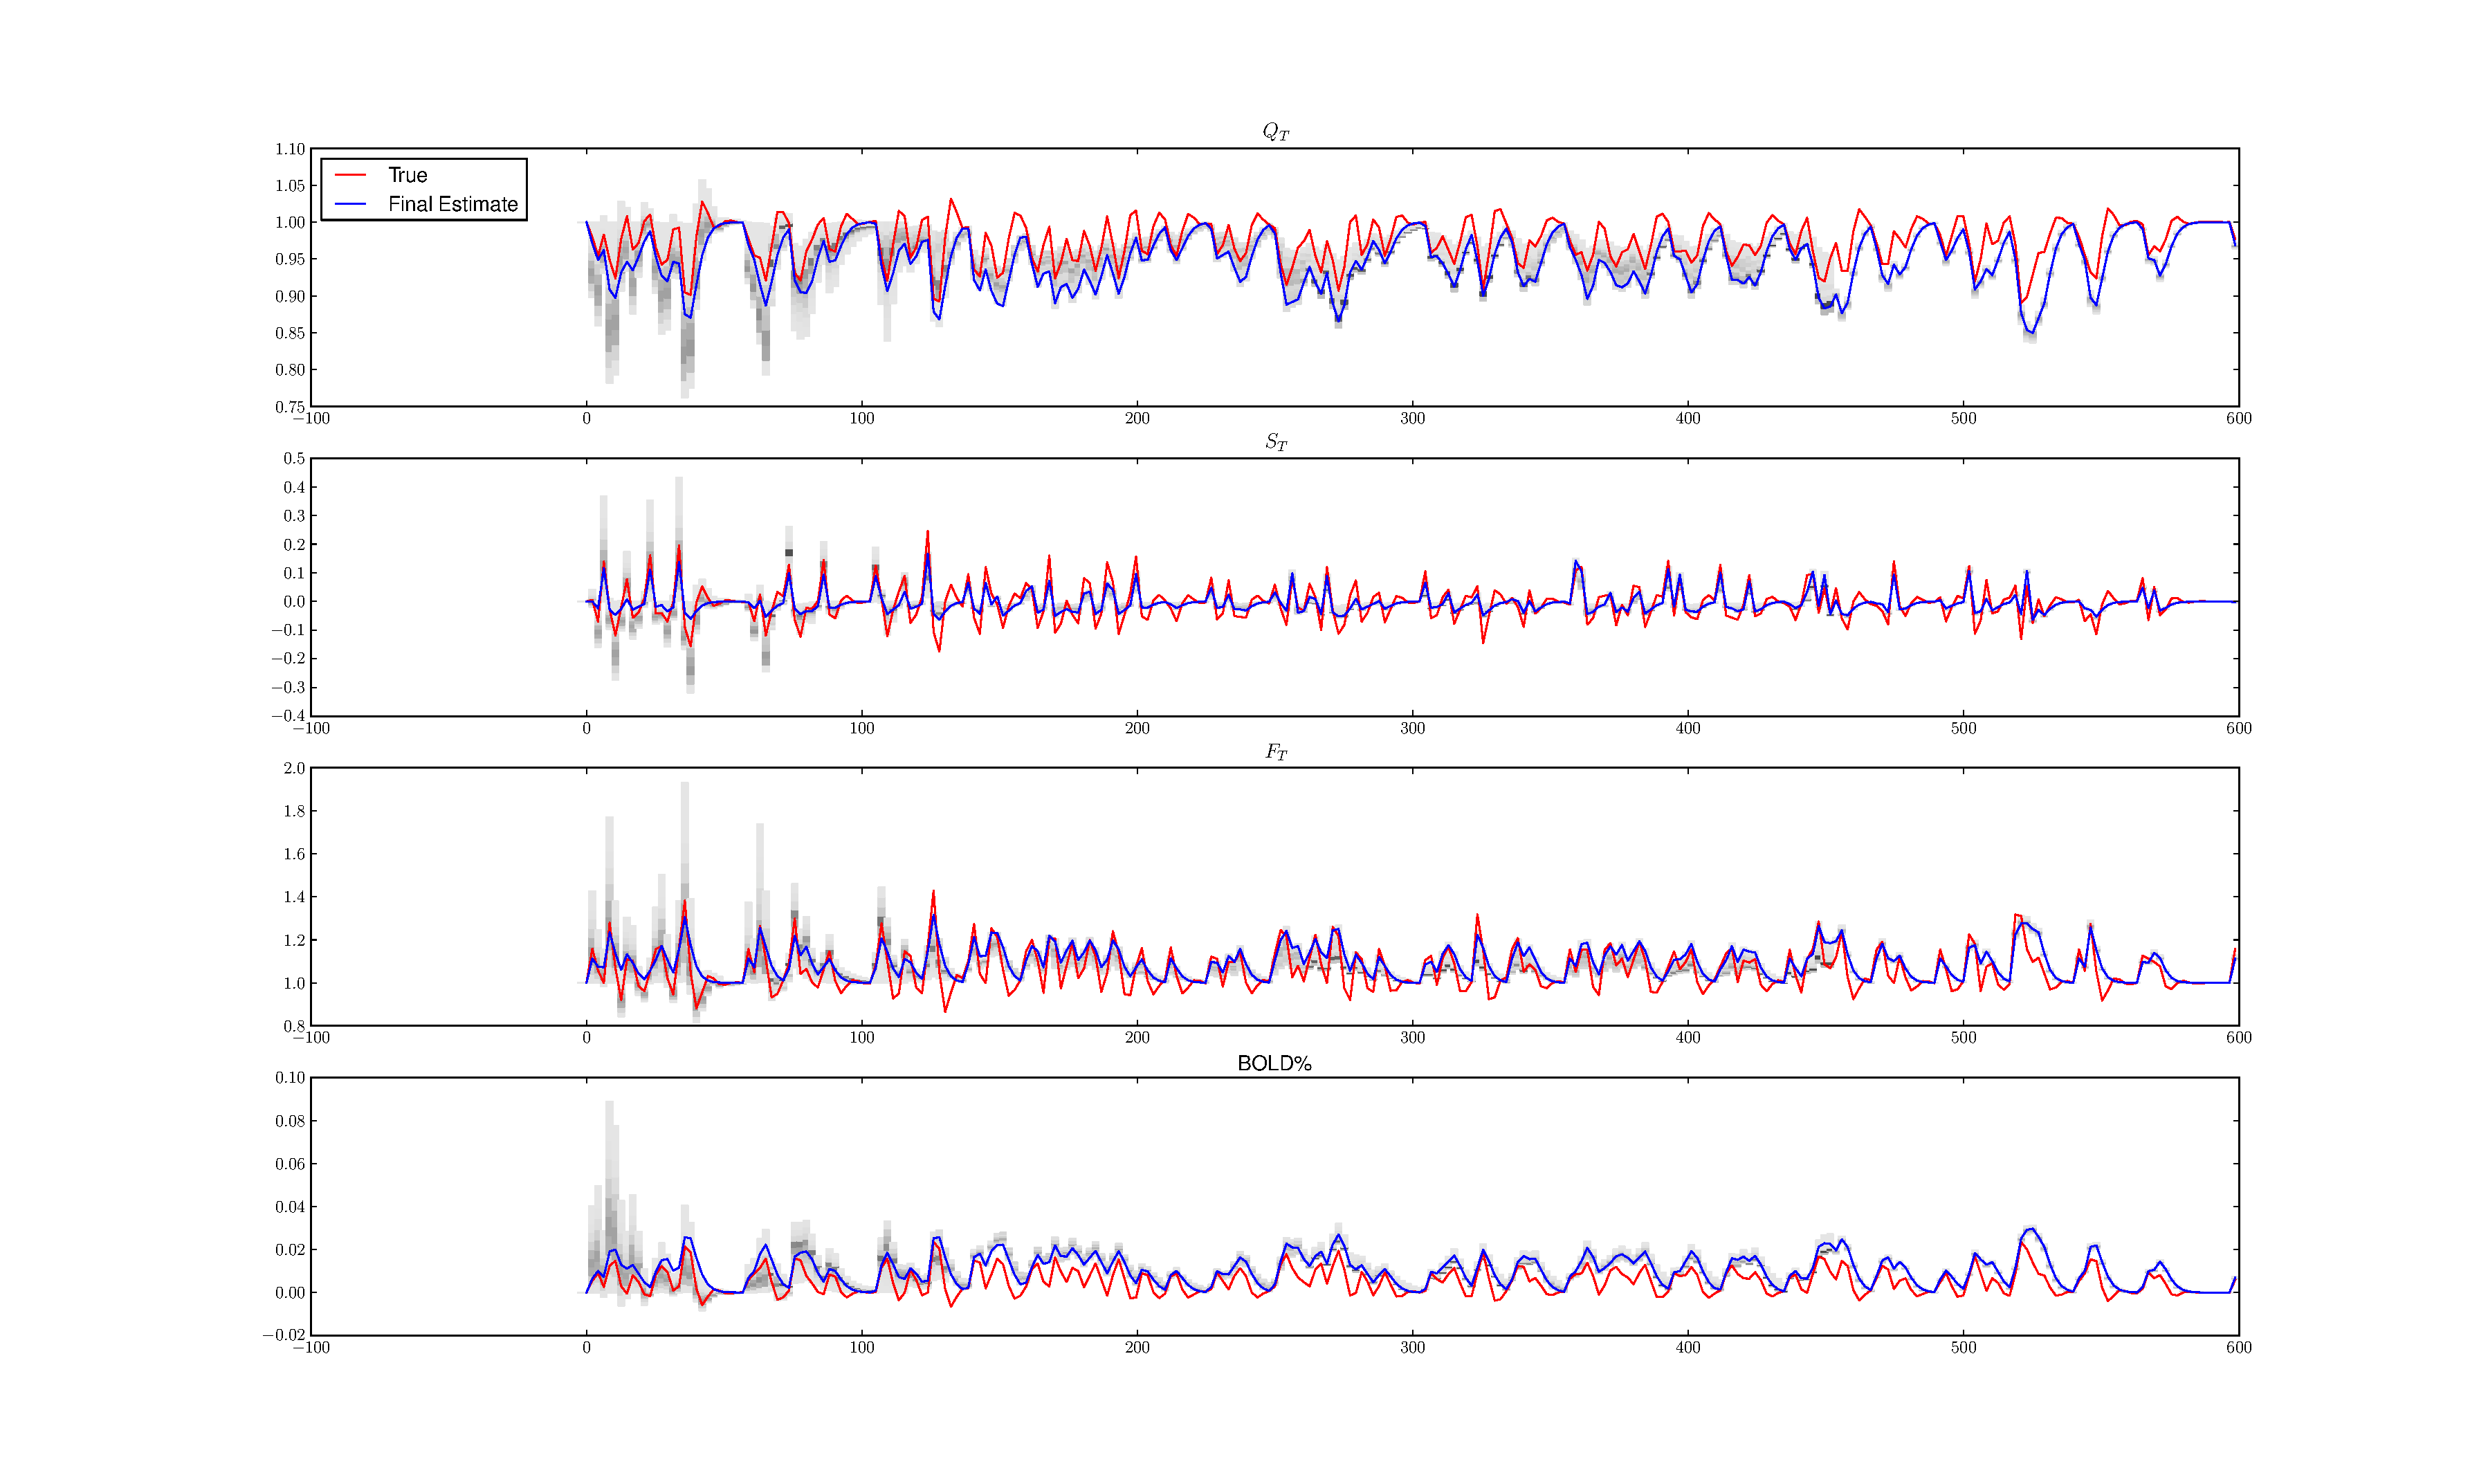
\includegraphics[trim=7cm 3cm 7cm 2cm, width=15cm]{images/highnoise_run6_3}}
\label{fig:ConvergenceRuns2}
\caption{Converging histogram for parameters during run 2, as in \autoref{fig:NoiseComparisonJustTwo}.}
\end{figure}

The parameters arrived at for all ten filter runs are shown in \autoref{tab:HighNoiseResults}.

\begin{table}[t]
\centering
\begin{tabular}{|c | c | c | c | c | c | c | c | c | c |}
\hline 
$\tau_0$ & $\alpha$ & $E_0$    & $V_0$    & $\tau_s$ & $\tau_f$ & $\epsilon$  & $ \sum \tau $ & $\sqrt{MSE}$ (Res.) & $\sqrt{MSE}$\\
\hline 
\rowcolor[gray]{.8}
1.45 & .3 & .47 & .044 & 1.94 & 1.99 & 1.8  & 5.38 &  & \\
\hline 
\hline 
1.19002 & 0.23495 & 0.42228 & 0.128 & 1.01468 & 2.47795 & 1.11677 & 4.68265   &0.0140648  &0.01572919   \\
0.9721 & 0.21902 & 0.30505 & 0.061 & 0.57801 & 1.99596 & 3.46135 & 3.54608    &0.0137314  &0.01377685   \\
1.57947 & 0.14153 & 0.33798 & 0.1079 & 0.5843 & 2.12475 & 1.78343 & 4.28852   &0.01275372 &0.01577449   \\
1.10937 & 0.2374 & 0.53491 & 0.0351 & 1.21862 & 3.07365 & 2.35039 & 5.40164   &0.0167258  &0.0115433    \\
1.10712 & 0.27535 & 0.33651 & 0.03161 & 1.50567 & 2.65181 & 4.19099 & 5.2646  &0.01369793 &0.01221607   \\
0.58026 & 0.47931 & 0.41354 & 0.11894 & 0.97563 & 3.69018 & 1.00084 & 5.24607 &0.01149511 &0.01315637   \\
\rowcolor[rgb]{.9,.5,.5}
1.29515 & 0.25957 & 0.27559 & 0.25952 & 1.70265 & 2.8458 & 0.66172 & 5.84361  &0.01555035 &0.01789781   \\
\rowcolor[rgb]{.5,.5,.9}
1.5185 & 0.21987 & 0.28348 & 0.07417 & 0.88822 & 3.07706 & 1.73929 & 5.48378  &0.01205351 &0.01246202   \\
0.68736 & 0.3283 & 0.39786 & 0.15614 & 1.07781 & 3.1158 & 0.66432 & 4.88097   &0.01510364 &0.01257713   \\
1.01703 & 0.28497 & 0.34741 & 0.05672 & 1.58774 & 2.65157 & 2.28519 & 5.25634 &0.012493   &0.01343459   \\
0.99247 & 0.29795 & 0.32207 & 0.20943 & 0.42757 & 2.21081 & 1.01674 & 3.63085 &0.01216522 &0.01505545   \\
\hline                                                                          
1.09535 & 0.27075 & 0.36152 & 0.11259 & 1.05099 & 2.71958 & 1.84282 & 4.86592 &0.01362132  &0.01396575\\
\hline 
\end{tabular}
\caption{Estimated Parameters on 10 different runs with high noise. First row is the true parameters.
Note also that the red row is Run 1 and the blue row is Run 2, as used named this section}
\label{tab:HighNoiseResults} 
\end{table}

\subsection{Pure-Noise, low magnitude}
The two final single-voxel test, forces the particle filter to attempt to "learn" a noise-only
timeseries. The noise used will be the same as that from the \autoref{sec:HighNoise},
$\sigma_x = .01, \sigma_y = .005$. The parameters will be set the same as well, but the
stimulus/input will be set to 0 the entire time. For the particle filter, on the other hand,
the stimulus will be left as in the previous two sections. The questions is if the particle
filter is able to appropriately differentiate from a signal with noise. The noise timeseries
are shown in \autoref{fig:NoiseOnly}, the preprocessed versions are shown in \autoref{fig:NoiseOnlyPrep}.
\begin{figure}[H]
\label{fig:NoiseOnly}
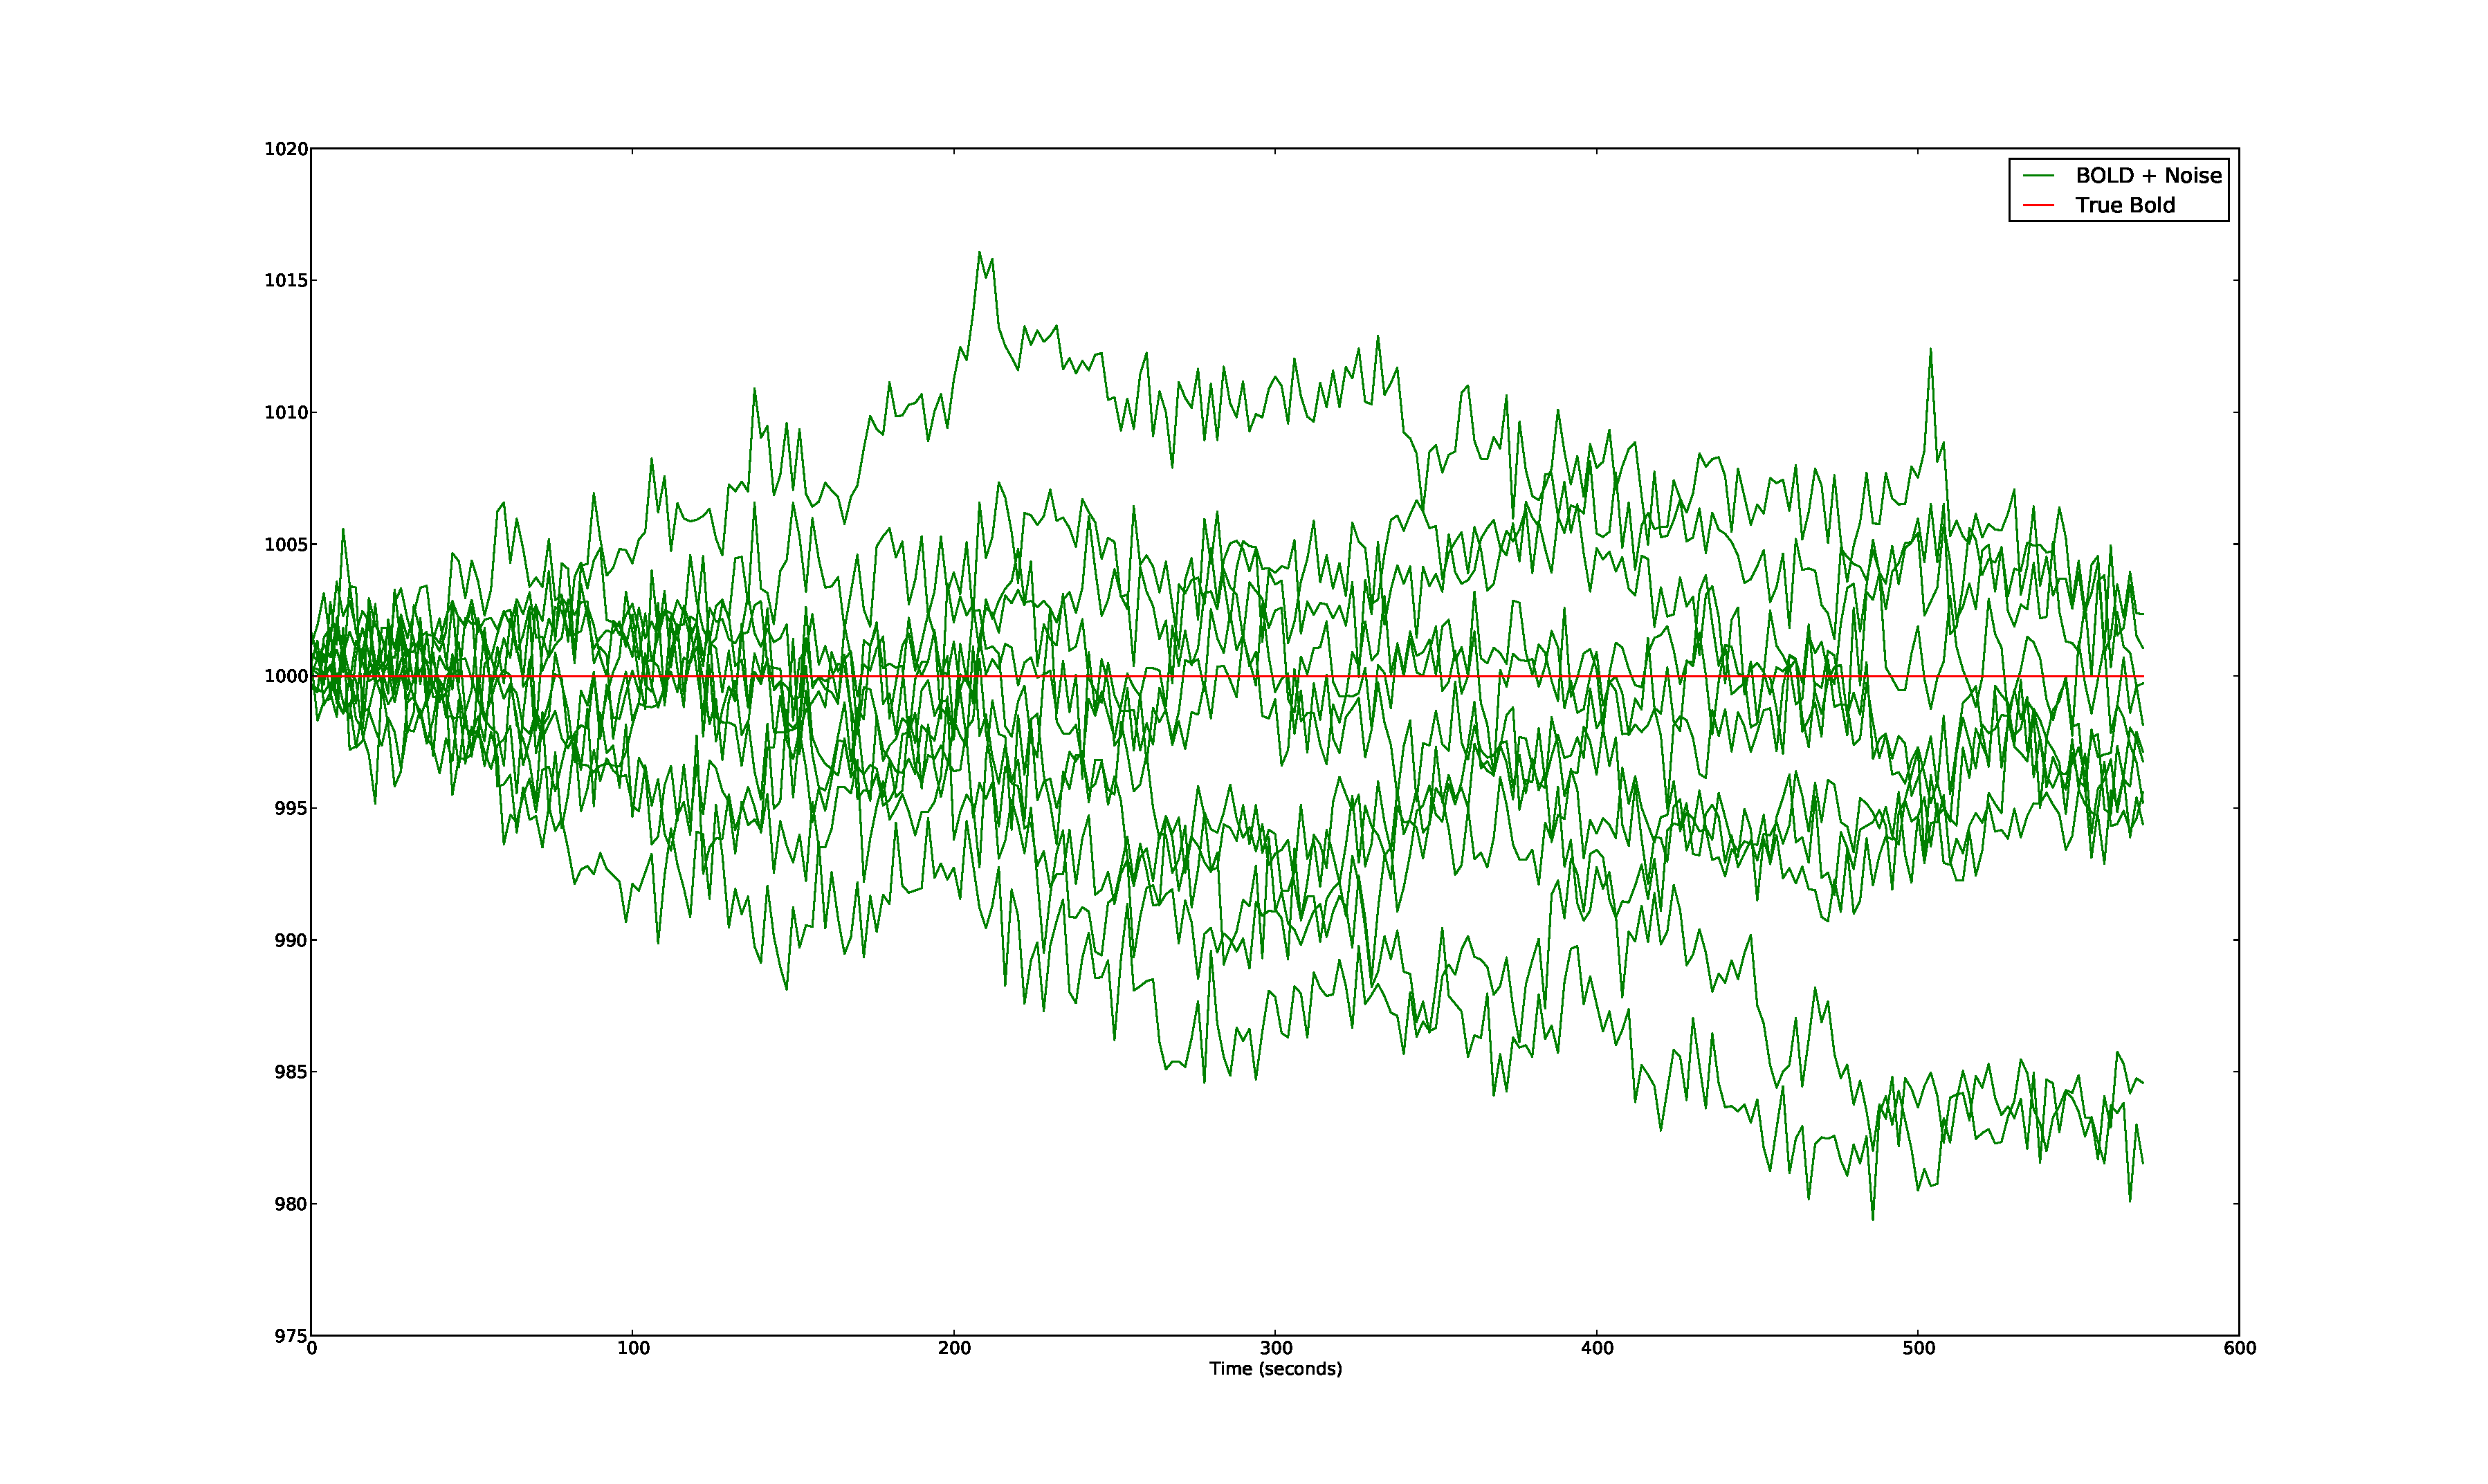
\includegraphics[trim=6cm 3cm 6cm 3cm,width=16cm]{images/realization_noiseonly}
\caption{Time-series lacking any real signal. With, $\sigma_x = .01, \sigma_y=.005$}
\end{figure}
\begin{figure}[H]
\label{fig:PreprocessedNoiseOnly}
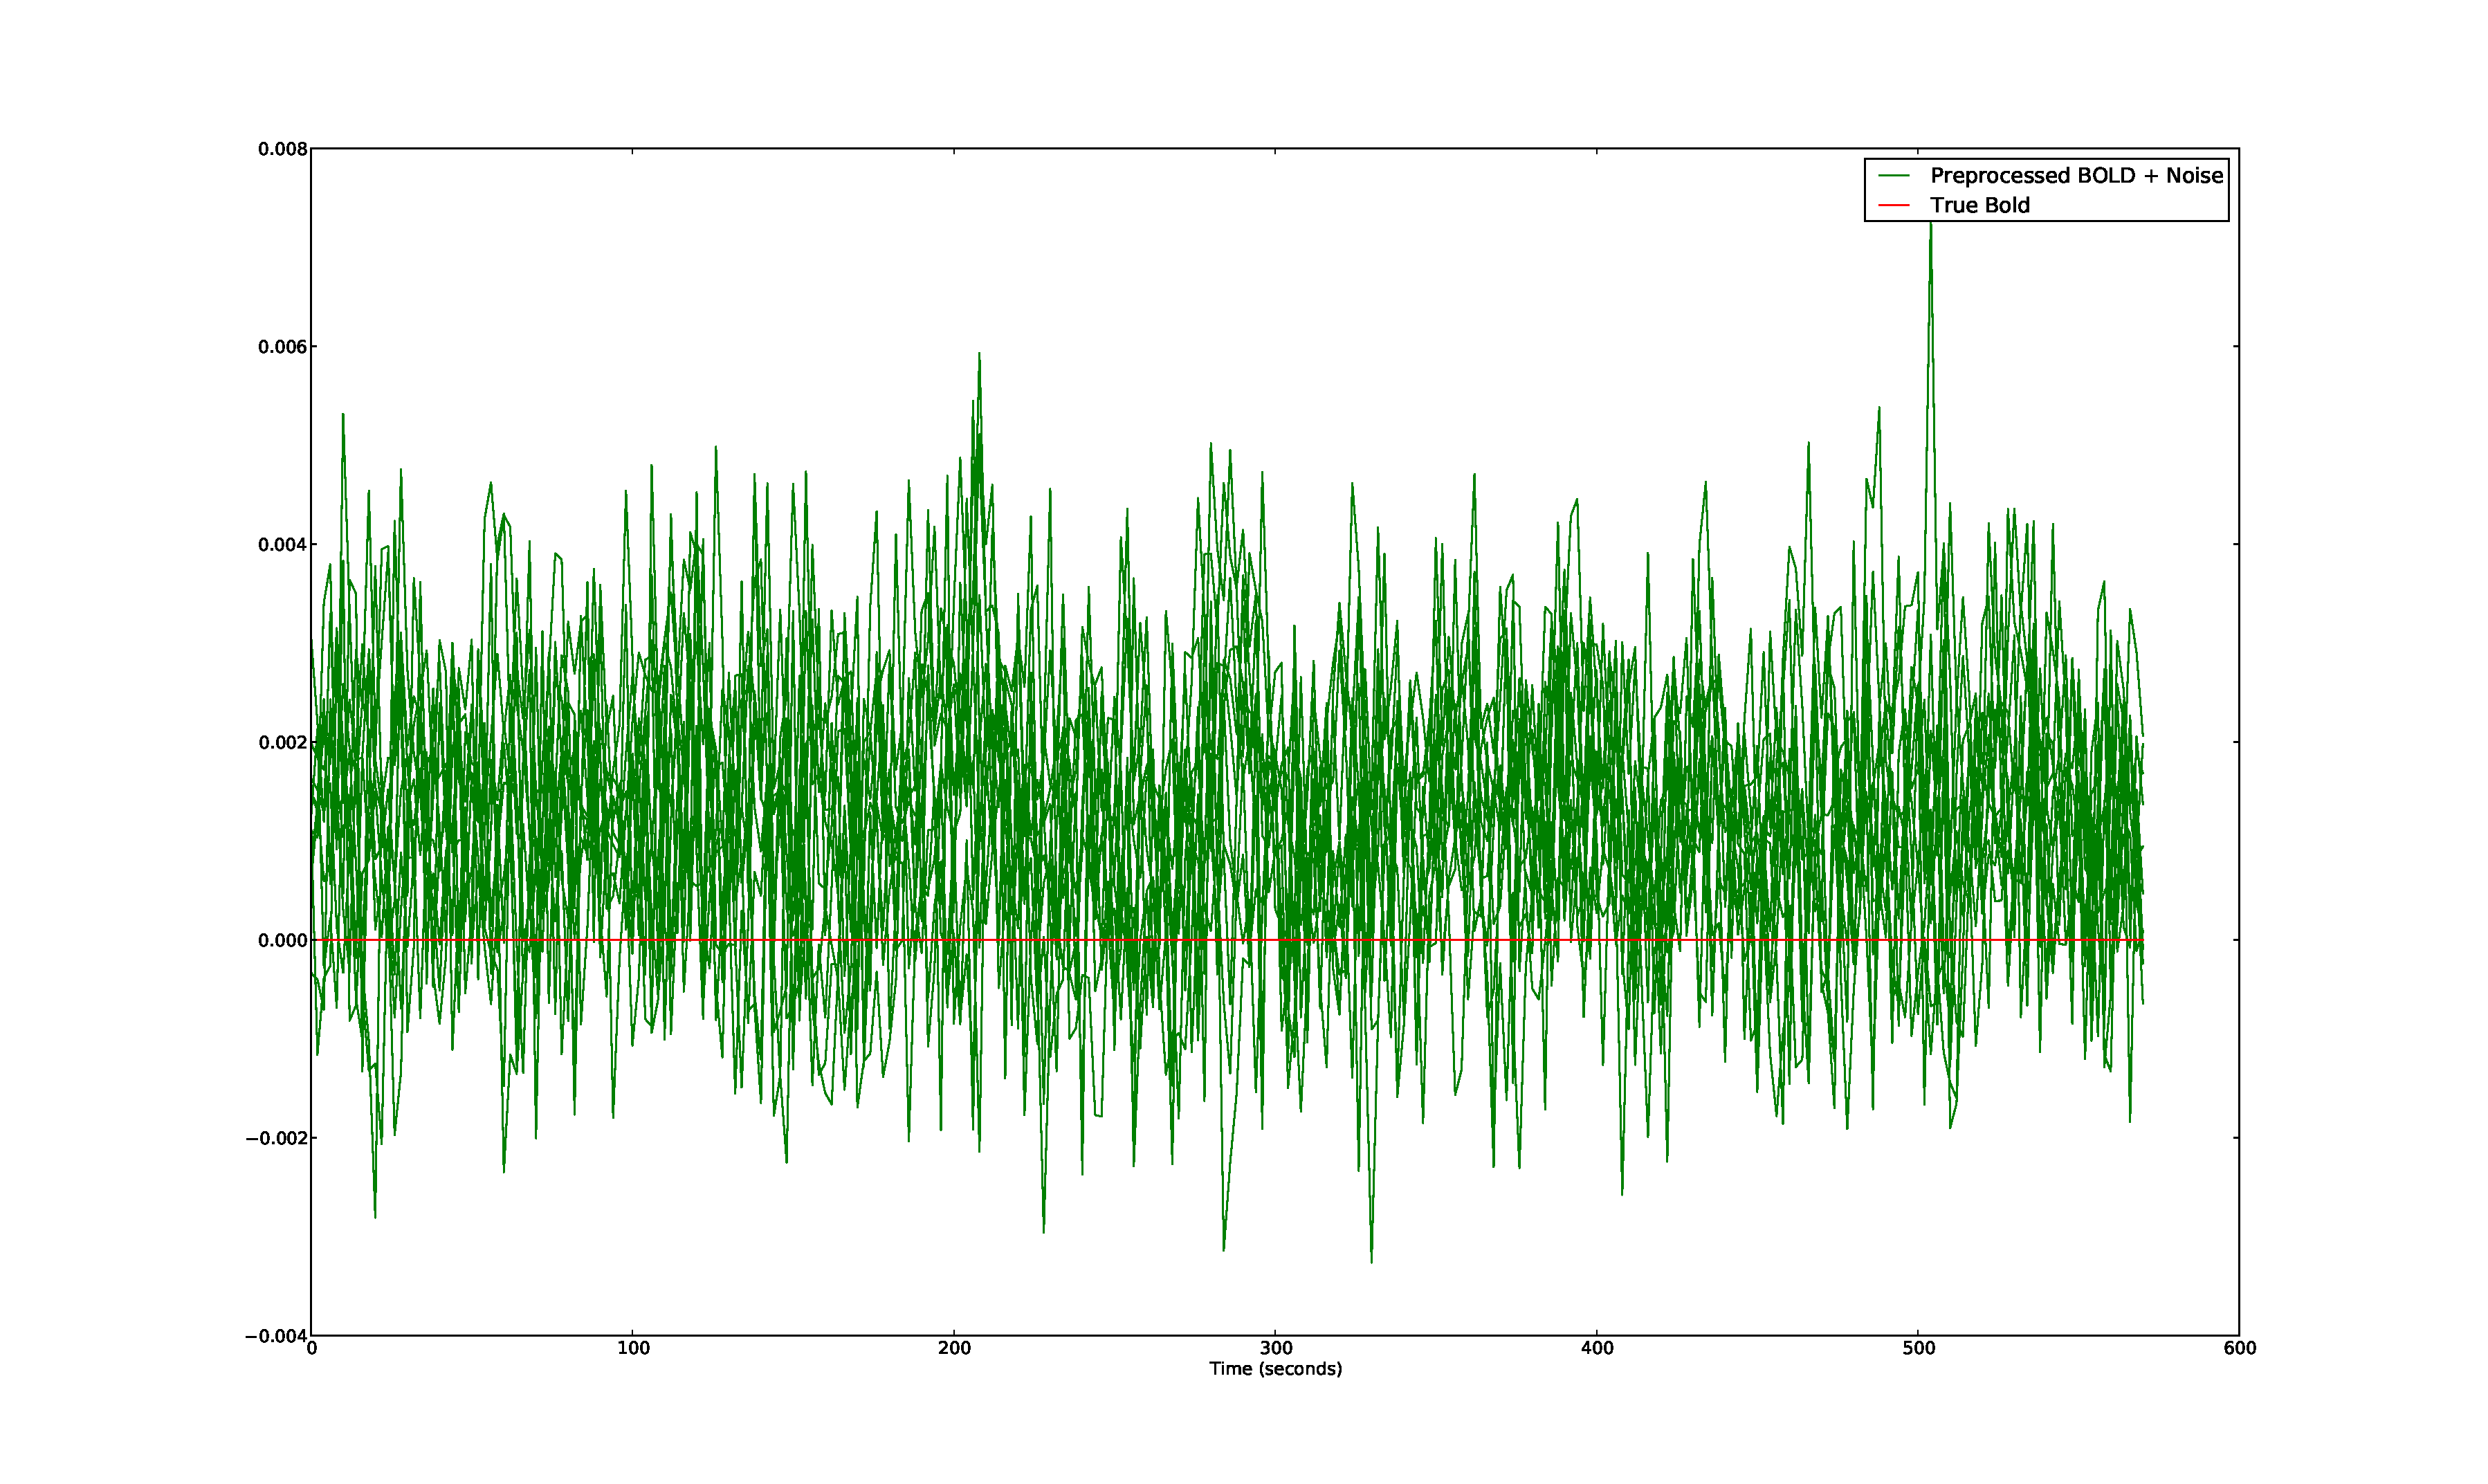
\includegraphics[trim=6cm 3cm 6cm 3cm,width=16cm]{images/preprocessed_noiseonly}
\caption{A comparison of the preprocessed signals for the signal-free case.}
\end{figure}

\begin{table}[t]
\centering
\begin{tabular}{|c | c | c | c | c | c | c | c | c |}
\hline 
$\tau_0$ & $\alpha$ & $E_0$    & $V_0$    & $\tau_s$ & $\tau_f$ & $\epsilon$  &  $\sqrt{MSE}$   \\
\hline 
1.0324 & 0.33211 & 0.34058 & 0.03012 & 1.40665 & 2.52079 & 0.5311 & \\
 0.98189 & 0.33047 & 0.3386 & 0.03014 & 1.45707 & 2.47232 & 0.45049 & 0.00158551 \\
 1.0429 & 0.33224 & 0.34124 & 0.02946 & 1.4618 & 2.49245 & 0.43012 &  0.00165055 \\
 1.02054 & 0.3321 & 0.33484 & 0.02586 & 1.45848 & 2.48741 & 0.4193 &  0.00150604 \\
 1.0565 & 0.33405 & 0.33758 & 0.02791 & 1.43784 & 2.52545 & 0.47517 & 0.00151513 \\
 1.01867 & 0.33528 & 0.33918 & 0.02782 & 1.48345 & 2.49605 & 0.44209 &0.00155645 \\
 1.051 & 0.33038 & 0.33837 & 0.02985 & 1.47651 & 2.48621 & 0.42719 &  0.00158526 \\
 1.00281 & 0.32929 & 0.33988 & 0.0298 & 1.43519 & 2.49256 & 0.48899 & 0.00164299 \\
 1.00893 & 0.33273 & 0.33982 & 0.0289 & 1.42903 & 2.49754 & 0.45688 & 0.0016793  \\
 1.01289 & 0.33275 & 0.3376 & 0.02997 & 1.41188 & 2.49881 & 0.50628 & 0.00182622 \\
 1.10247 & 0.33371 & 0.3419 & 0.02939 & 1.43774 & 2.53384 & 0.44079 & 0.00195009 \\
\hline                                                                
1.03009 & 0.33228 & 0.33905 & 0.02902 & 1.44506 & 2.50031 & 0.46076 & 0.00165129 \\
\hline 
\end{tabular}
\caption{Estimated Parameters on 10 different runs with low noise. }
\label{tab:NoiseOnlyResults} 
\end{table}

The line fits are shown in \autoref{fig:fits_noiseonly}. Now the
low MSE and reasonableness of the parameters is cause for concern. Additionally, the precision
with which the convergence occurred is enviable, compared to the actual signals.
However, the impulse response, which has less importance in nonlinear systems, could
be usefull for separating out good voxels from bad. Note that in \autoref{fig:PreprocessedNoiseOnly}
peaks at well below $.005$, the standard deviation of the weighting function. Thus, the reason
the fits are in such agreement is that no convergence occurred at all, as 
further shown by \autoref{JustNoiseConvergence}. Thus one more test is necessary on
a signal with enough noise to actually be considered a signal. But first,
there is still the matter of identifying this noise-only voxel. Clearly MSE and
the parameters themselves don't have the information to differentiate in this case.
Thus the answer falls on either the final estimated variance (which will be high
because no particles strayed far from the center) or the impulse response.
I prefer the impulse response because it doesn't depend on something that 
may be less than dependable, namelay the rate of convergence.

\begin{figure}[H]
\label{fig:fits_noiseonly}
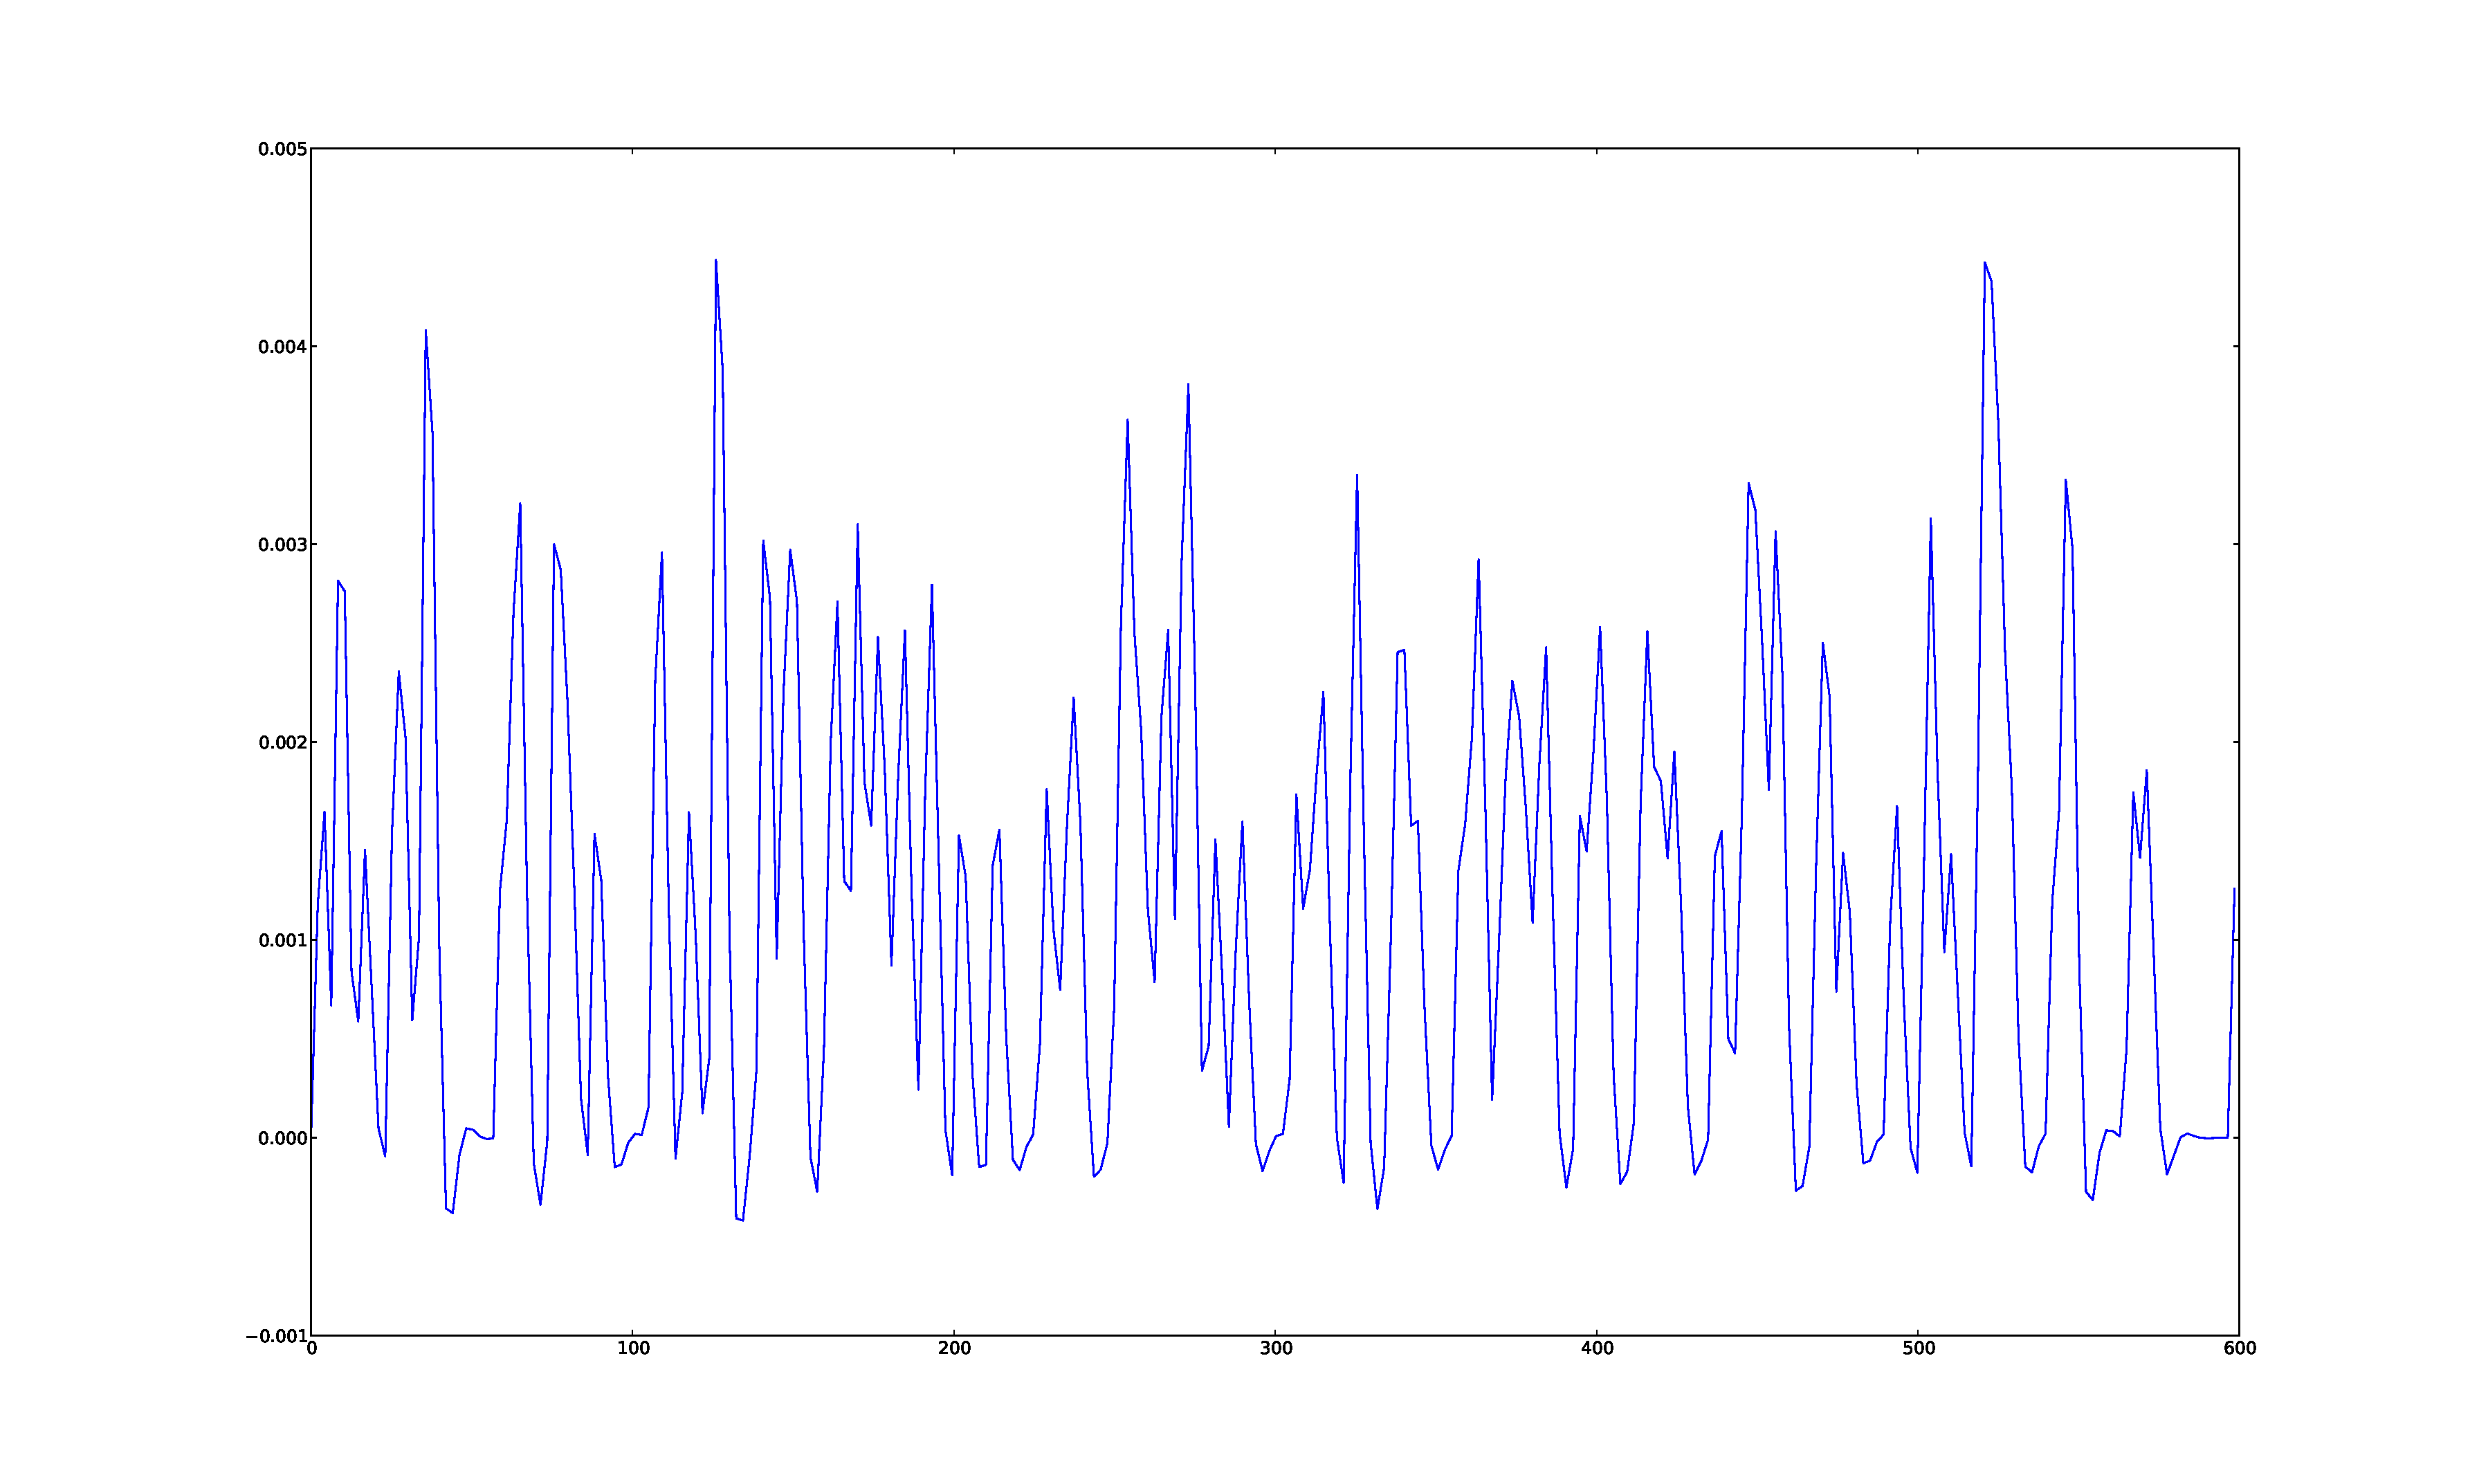
\includegraphics[trim=6cm 3cm 6cm 3cm,width=16cm]{images/fits_noiseonly}
\caption{Fits to the non-active, low noise signal. Note that the line is thick because all
the fits overlap. This is all 1 fitted lines.}
\end{figure}

\begin{figure}[H]
\label{fig:justnoise_fit_0}
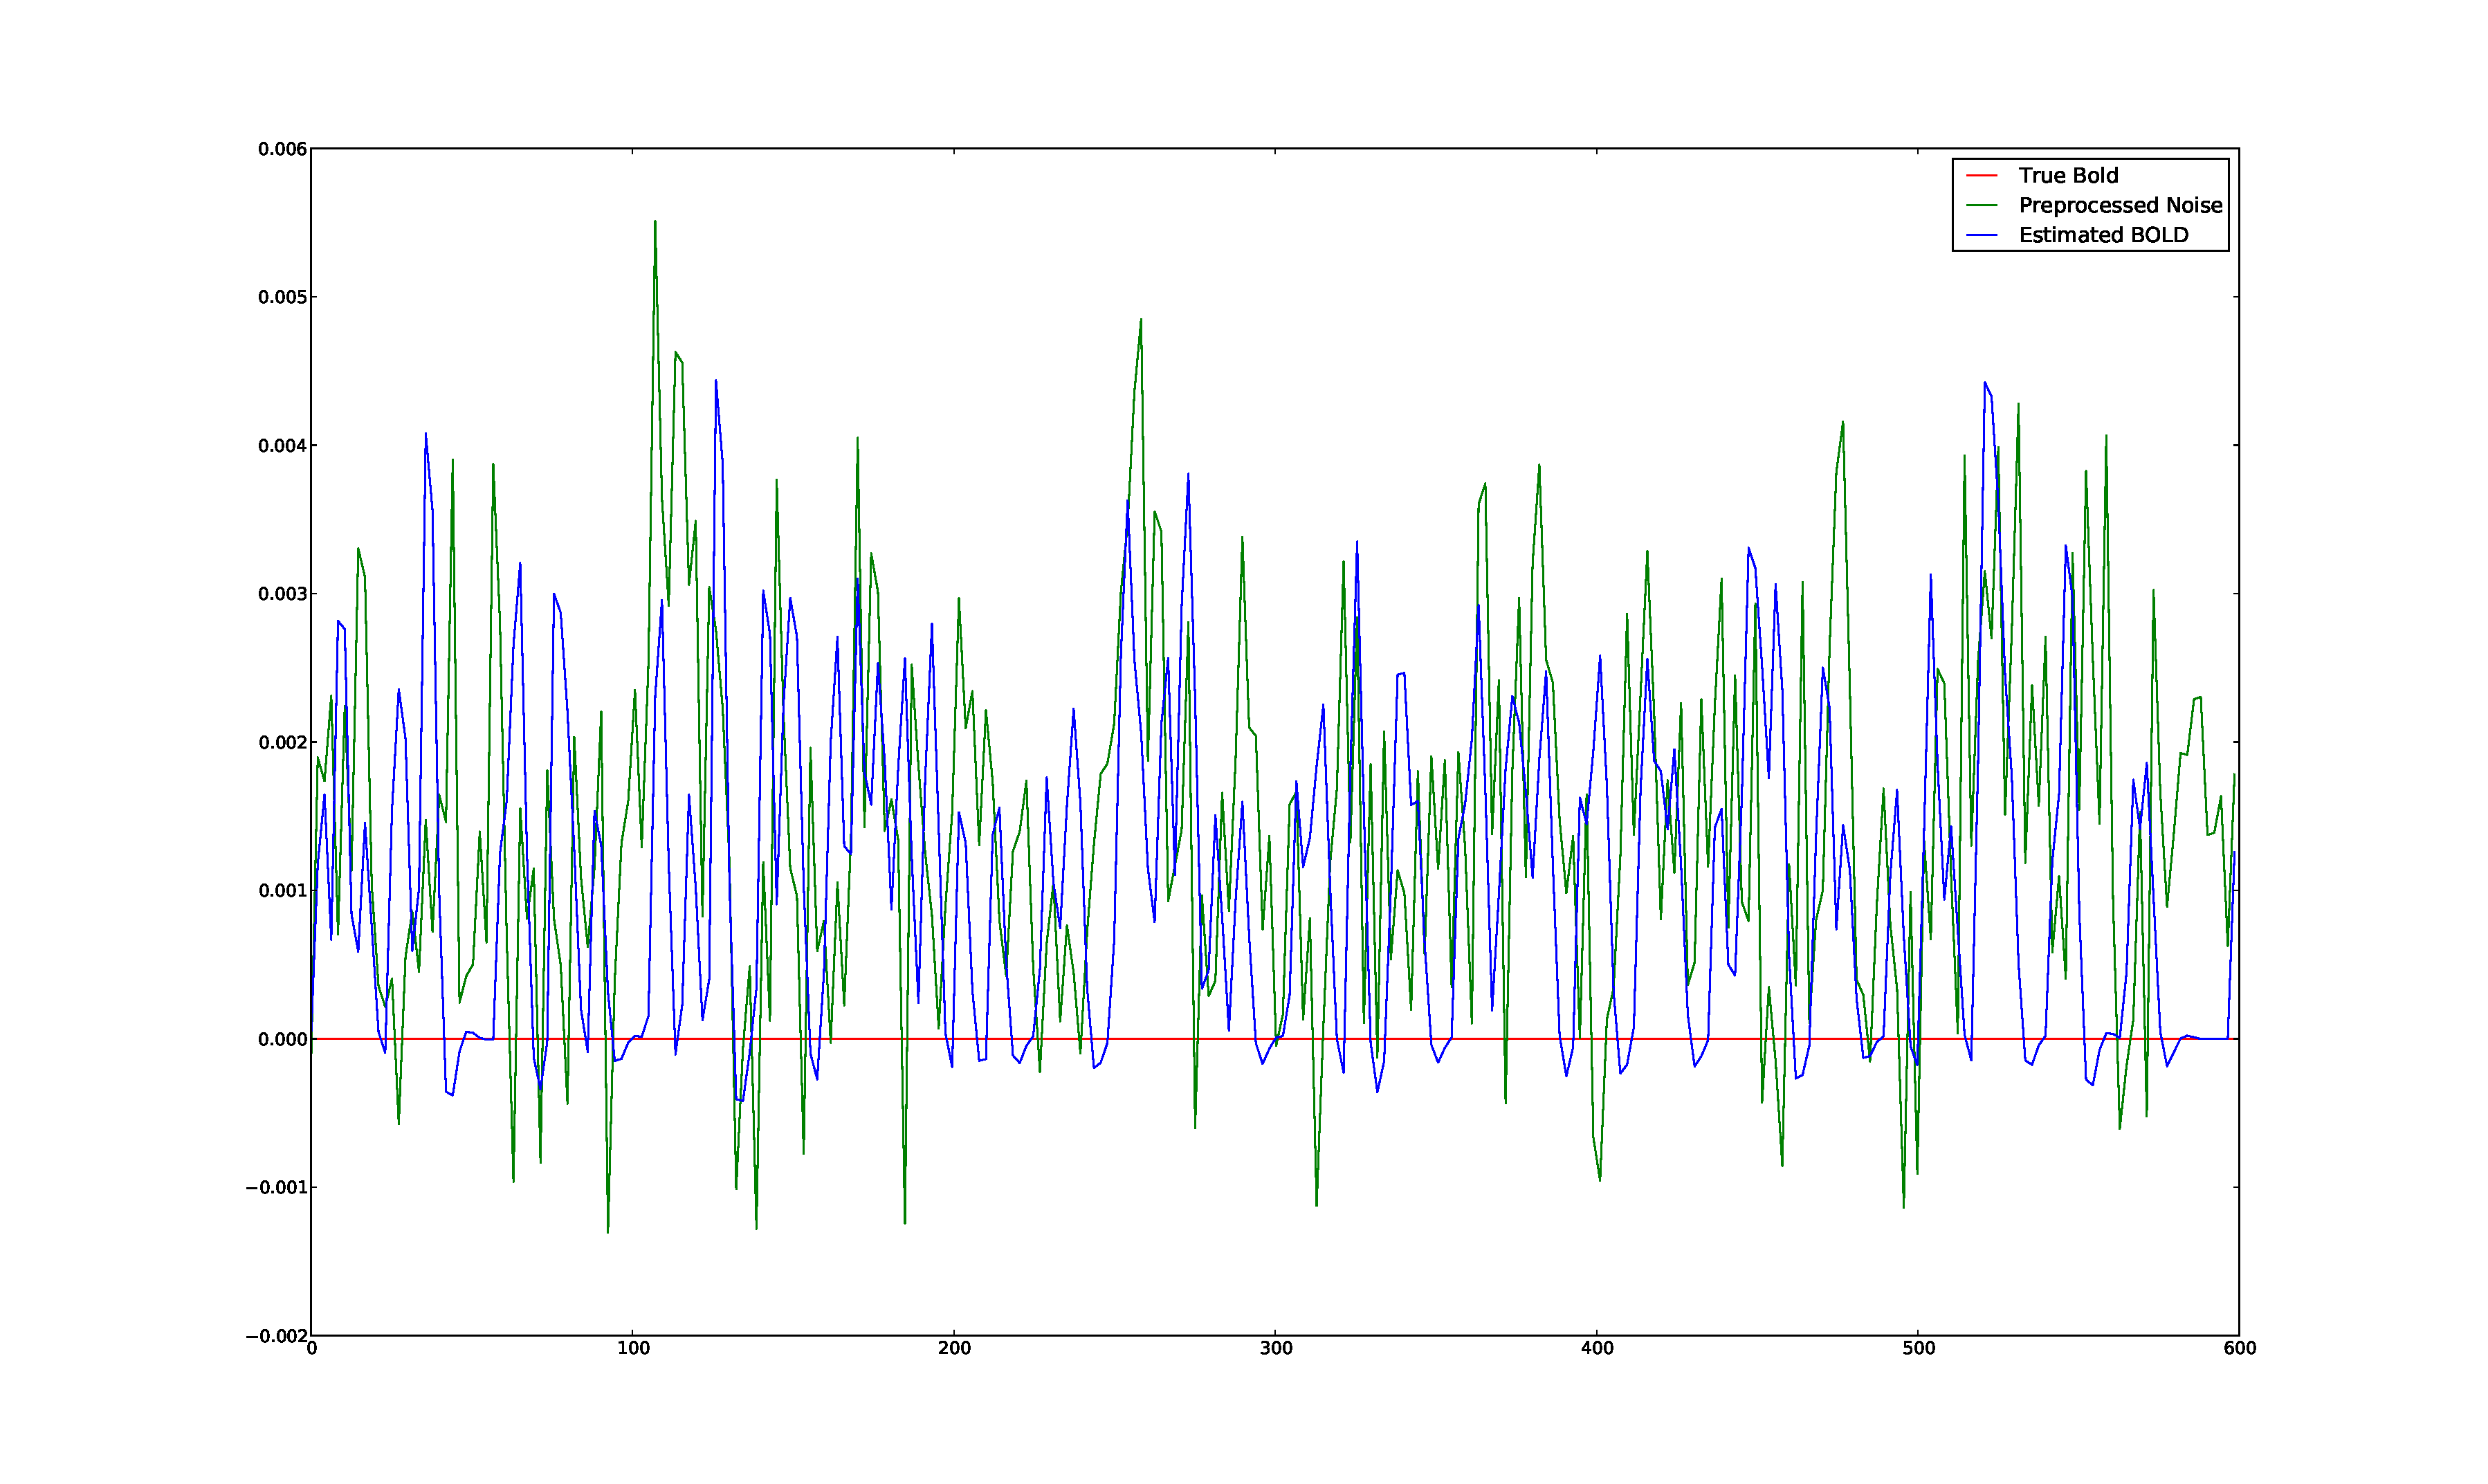
\includegraphics[trim=6cm 3cm 6cm 3cm,width=16cm]{images/justnoise_fit_0}
\caption{Fit from a single particle filter run, with the noise input. }
\end{figure} %uses allnoise/ALLNOISE-0-w0

\begin{figure}[H]
\subfigure[$\tau_0$, $\alpha$, $E_0$, $V_0$]
{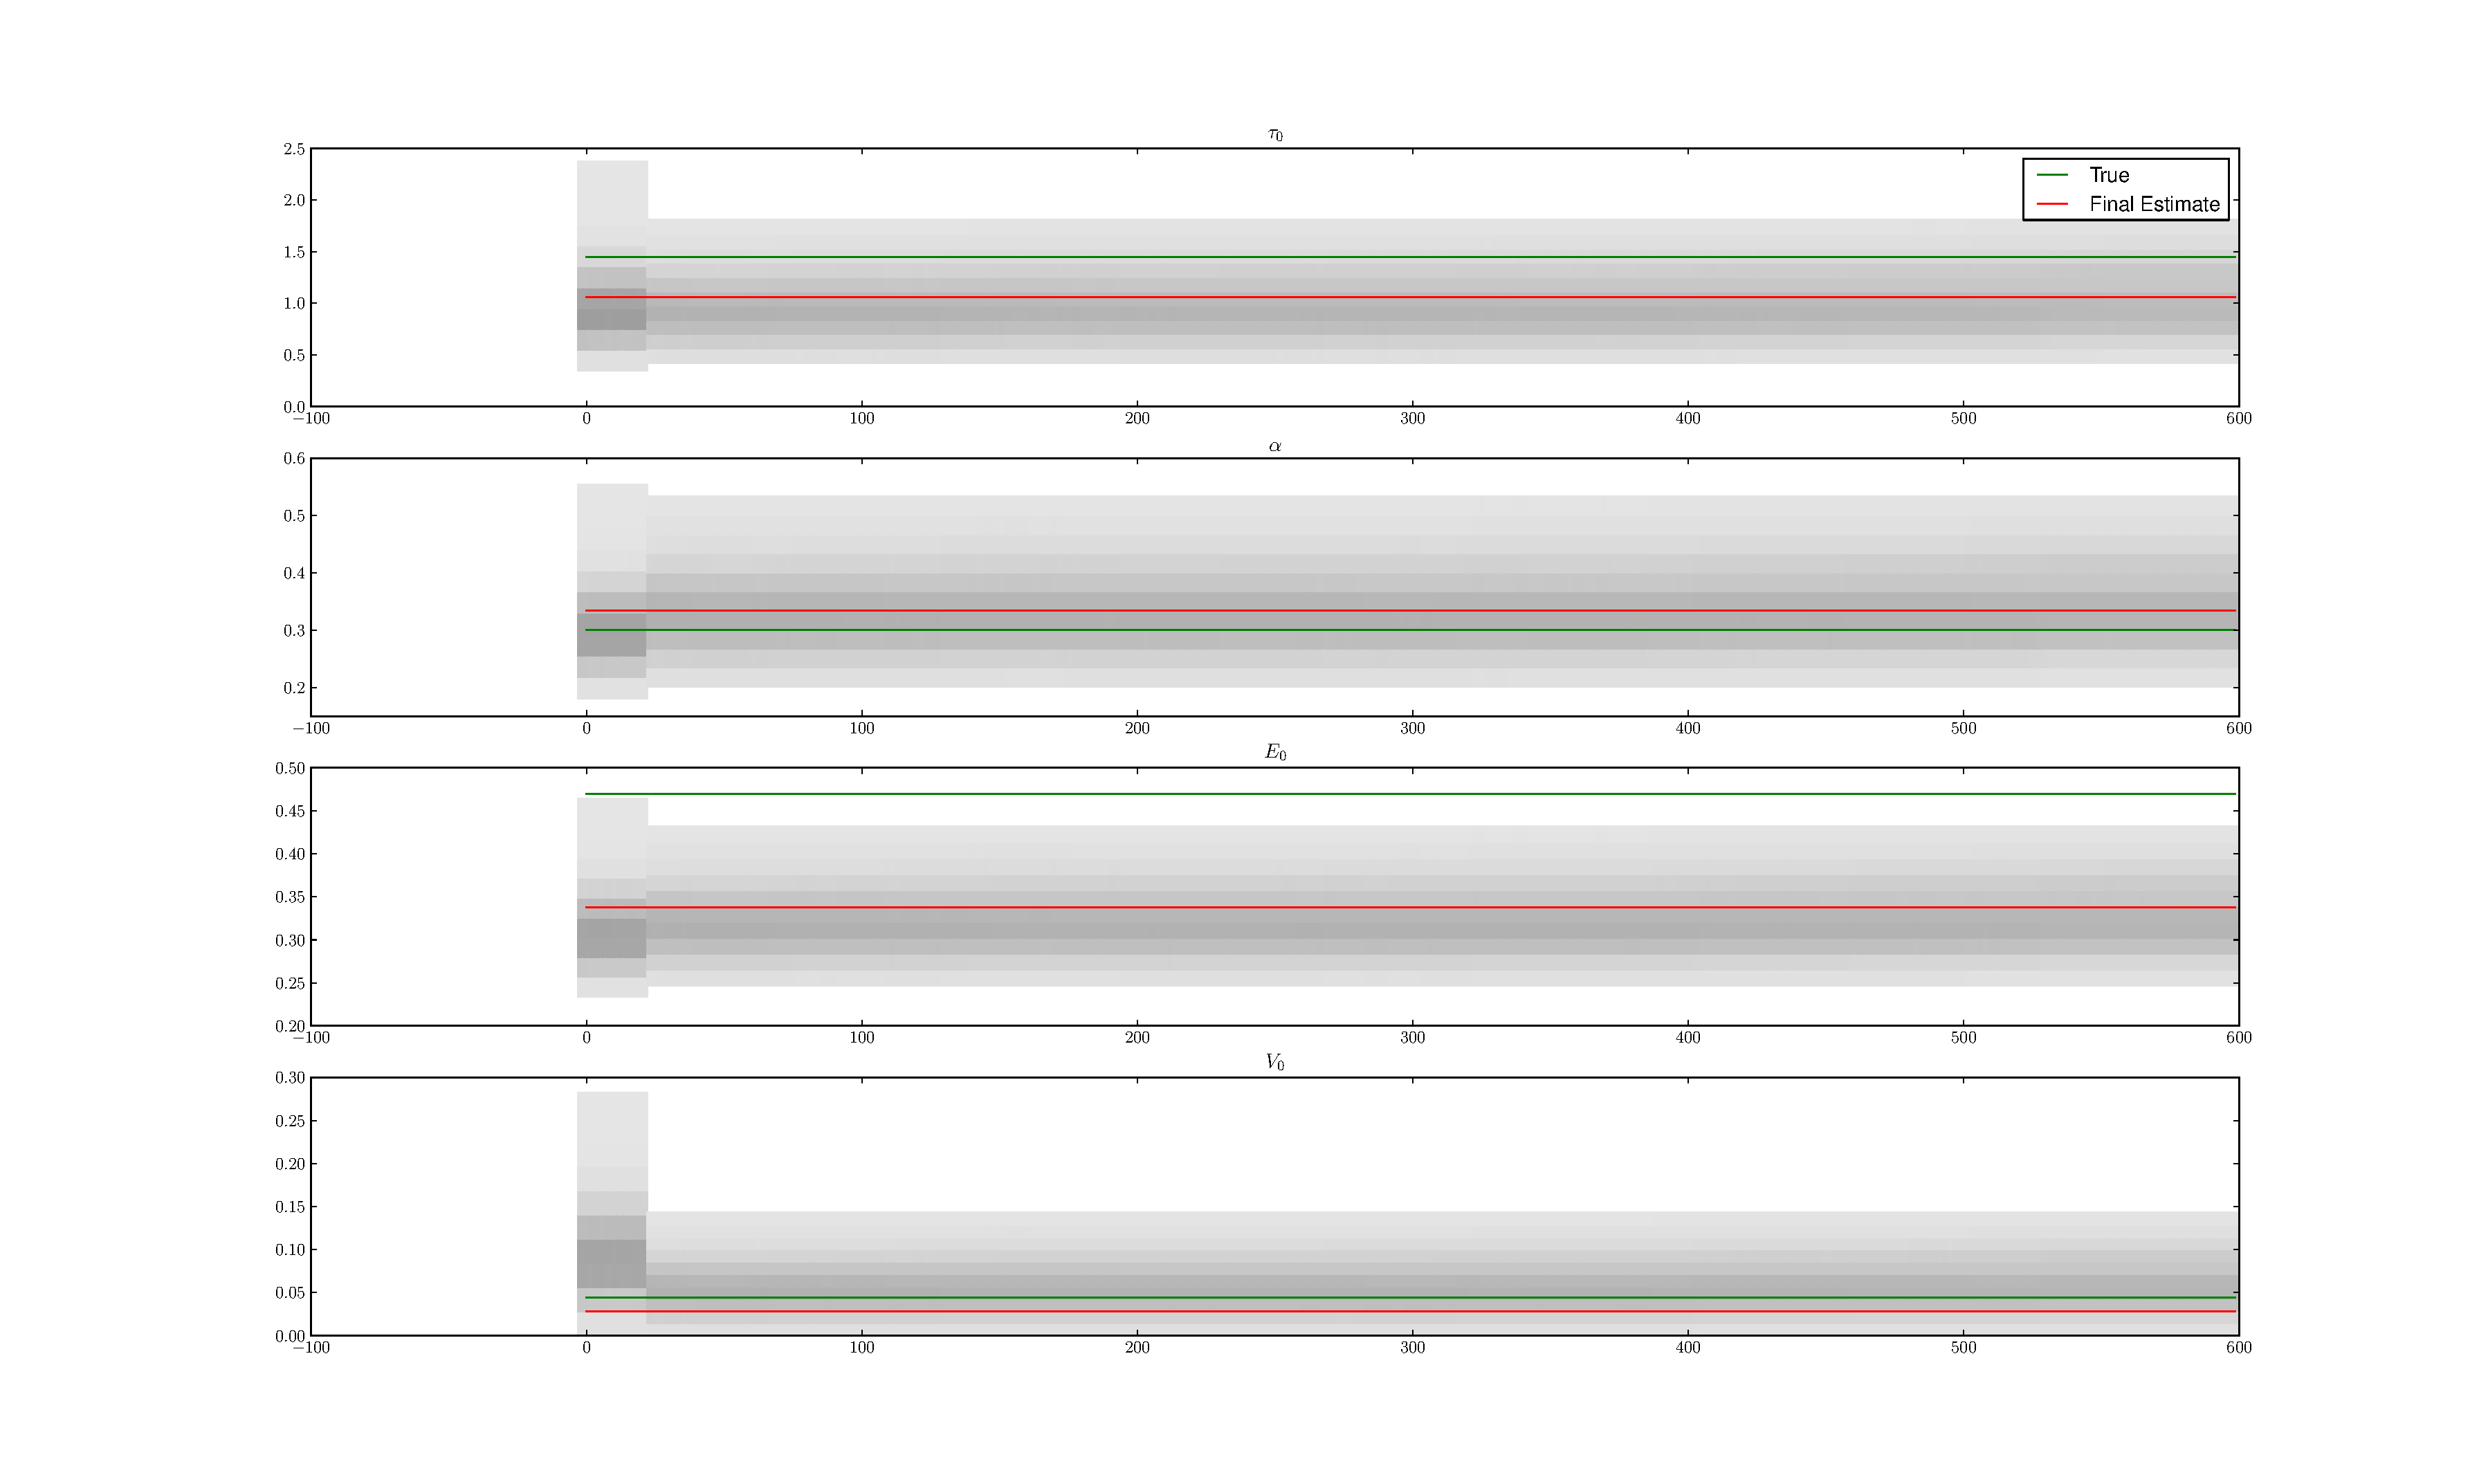
\includegraphics[trim=7cm 3cm 7cm 4cm, width=15cm]{images/justnoise_hist_1}}\\
\end{figure}
\begin{figure}[H]
\subfigure[$\tau_s$, $\tau_f$, $\epsilon$, $V$] 
{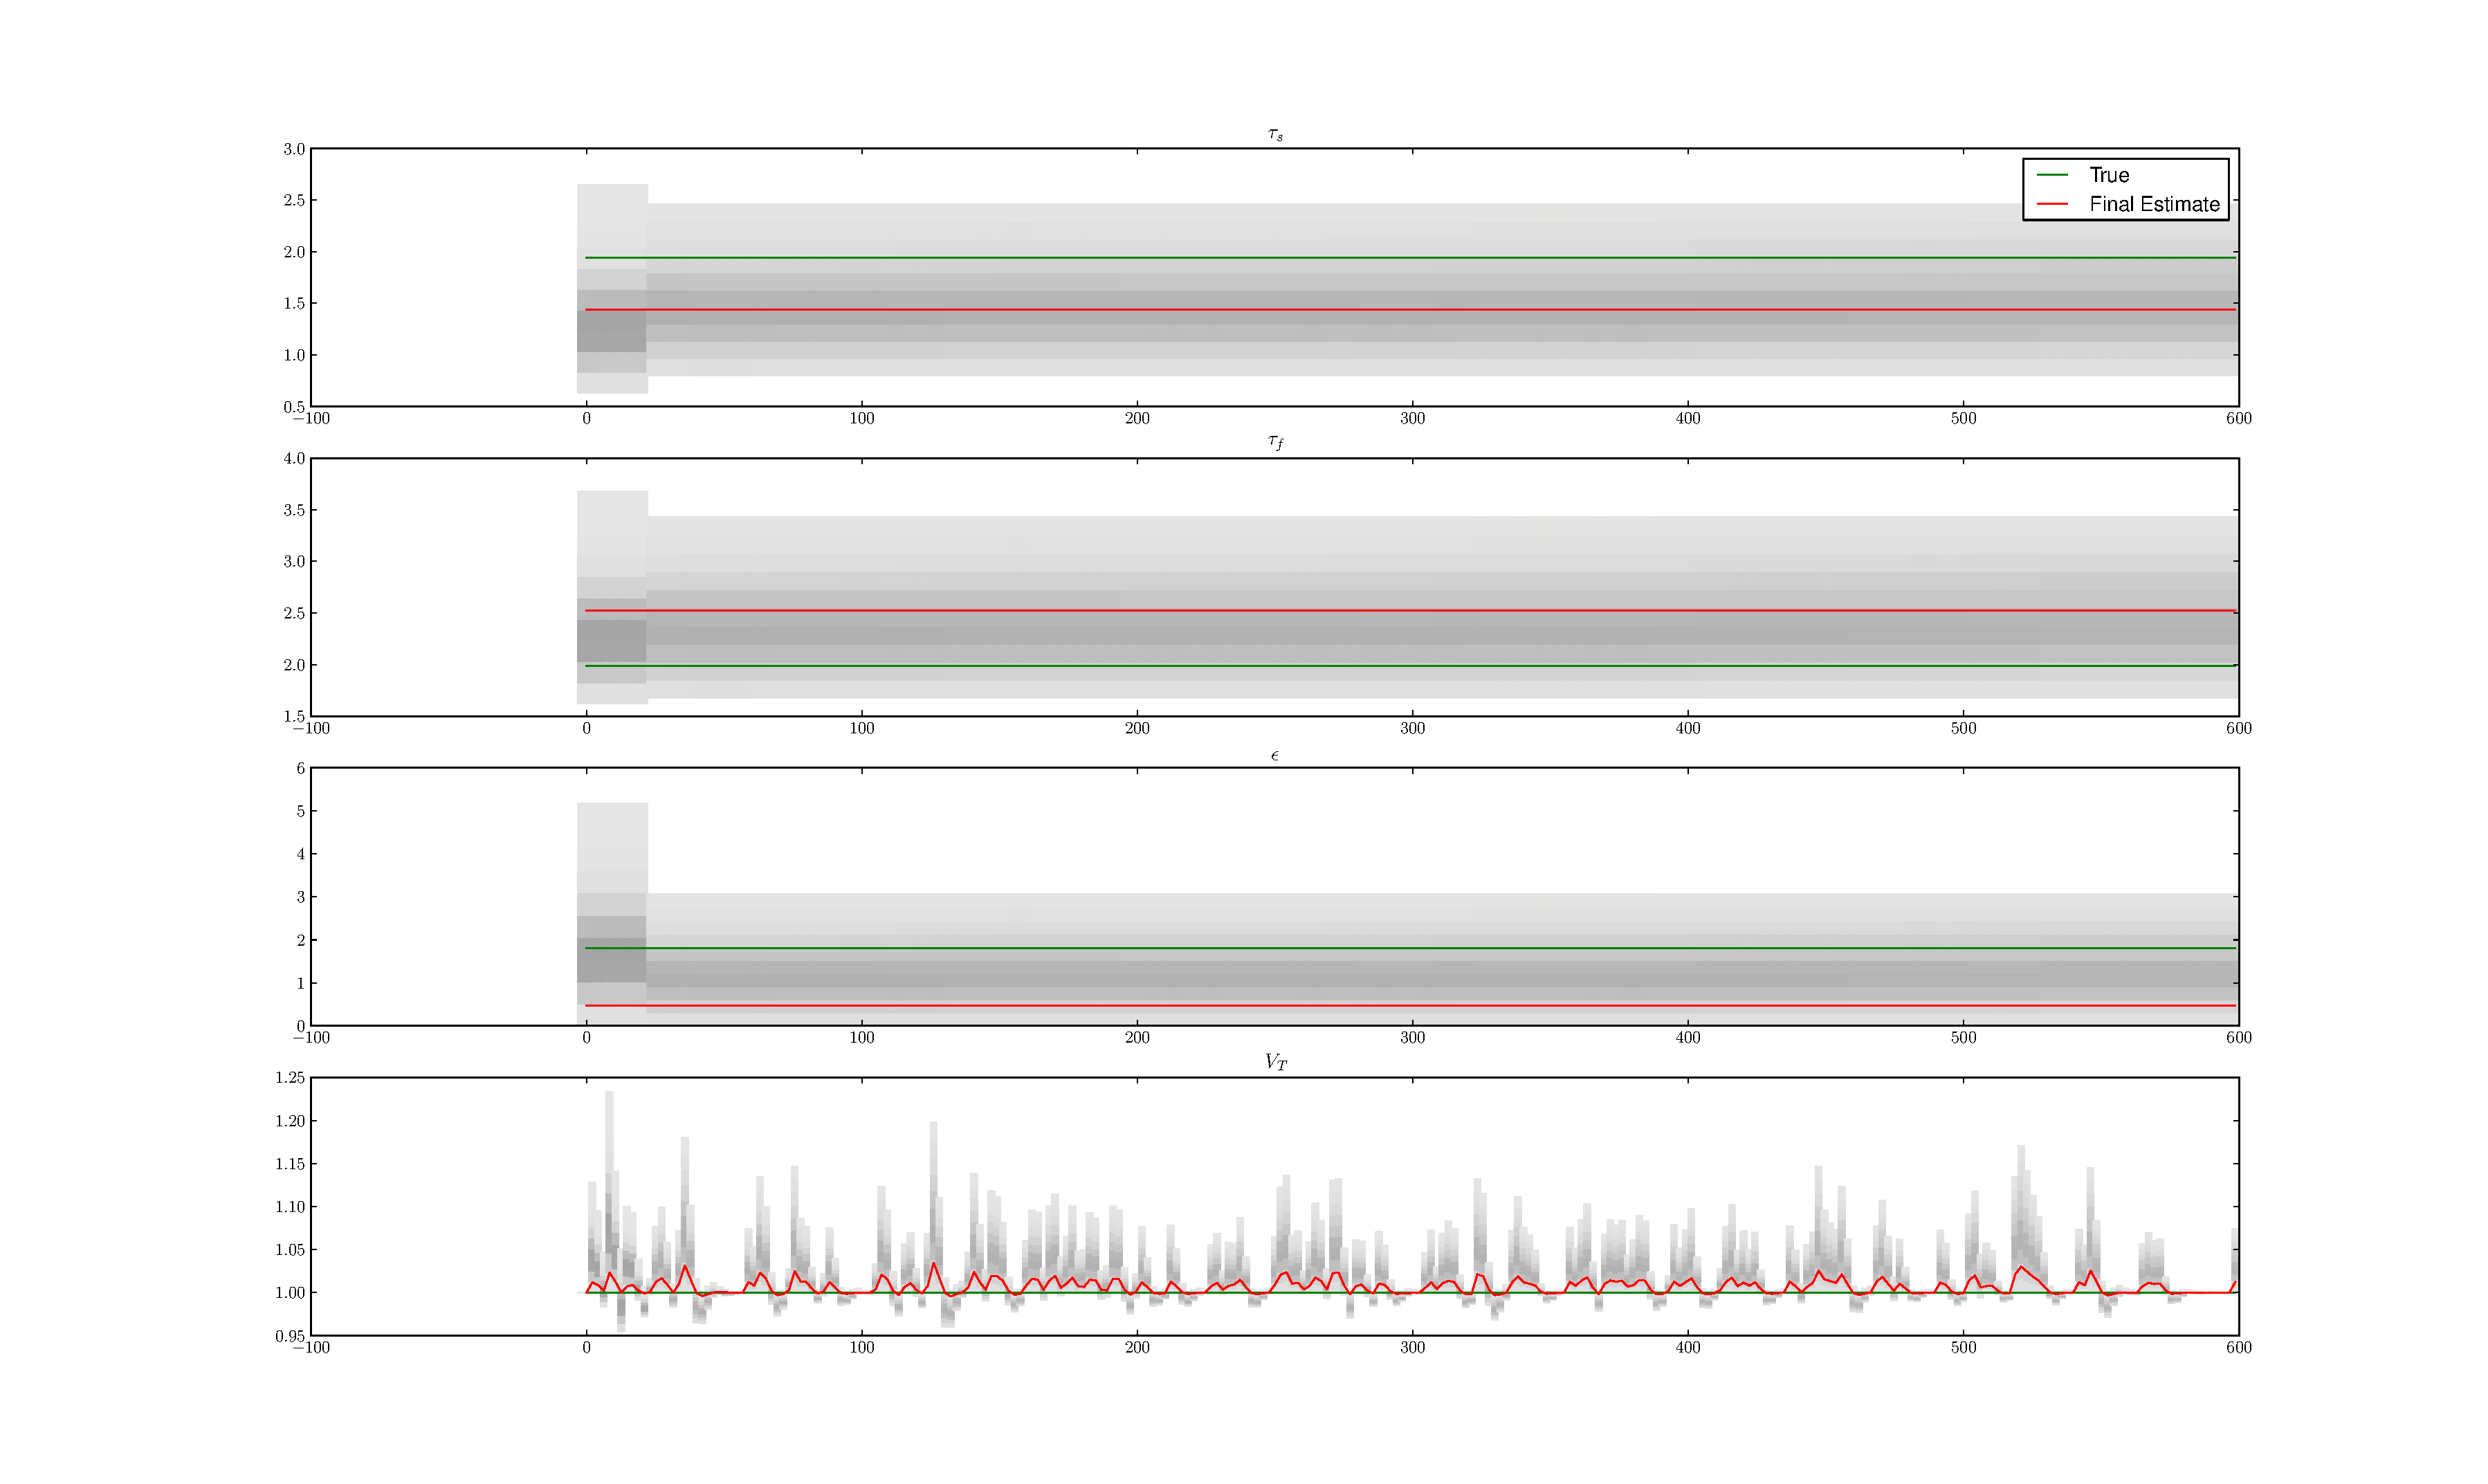
\includegraphics[trim=7cm 3cm 7cm 1cm, width=15cm]{images/justnoise_hist_2}}\\
\end{figure}
\begin{figure}[H]
\subfigure[$Q$, $S$, $F$, $BOLD$ ]
{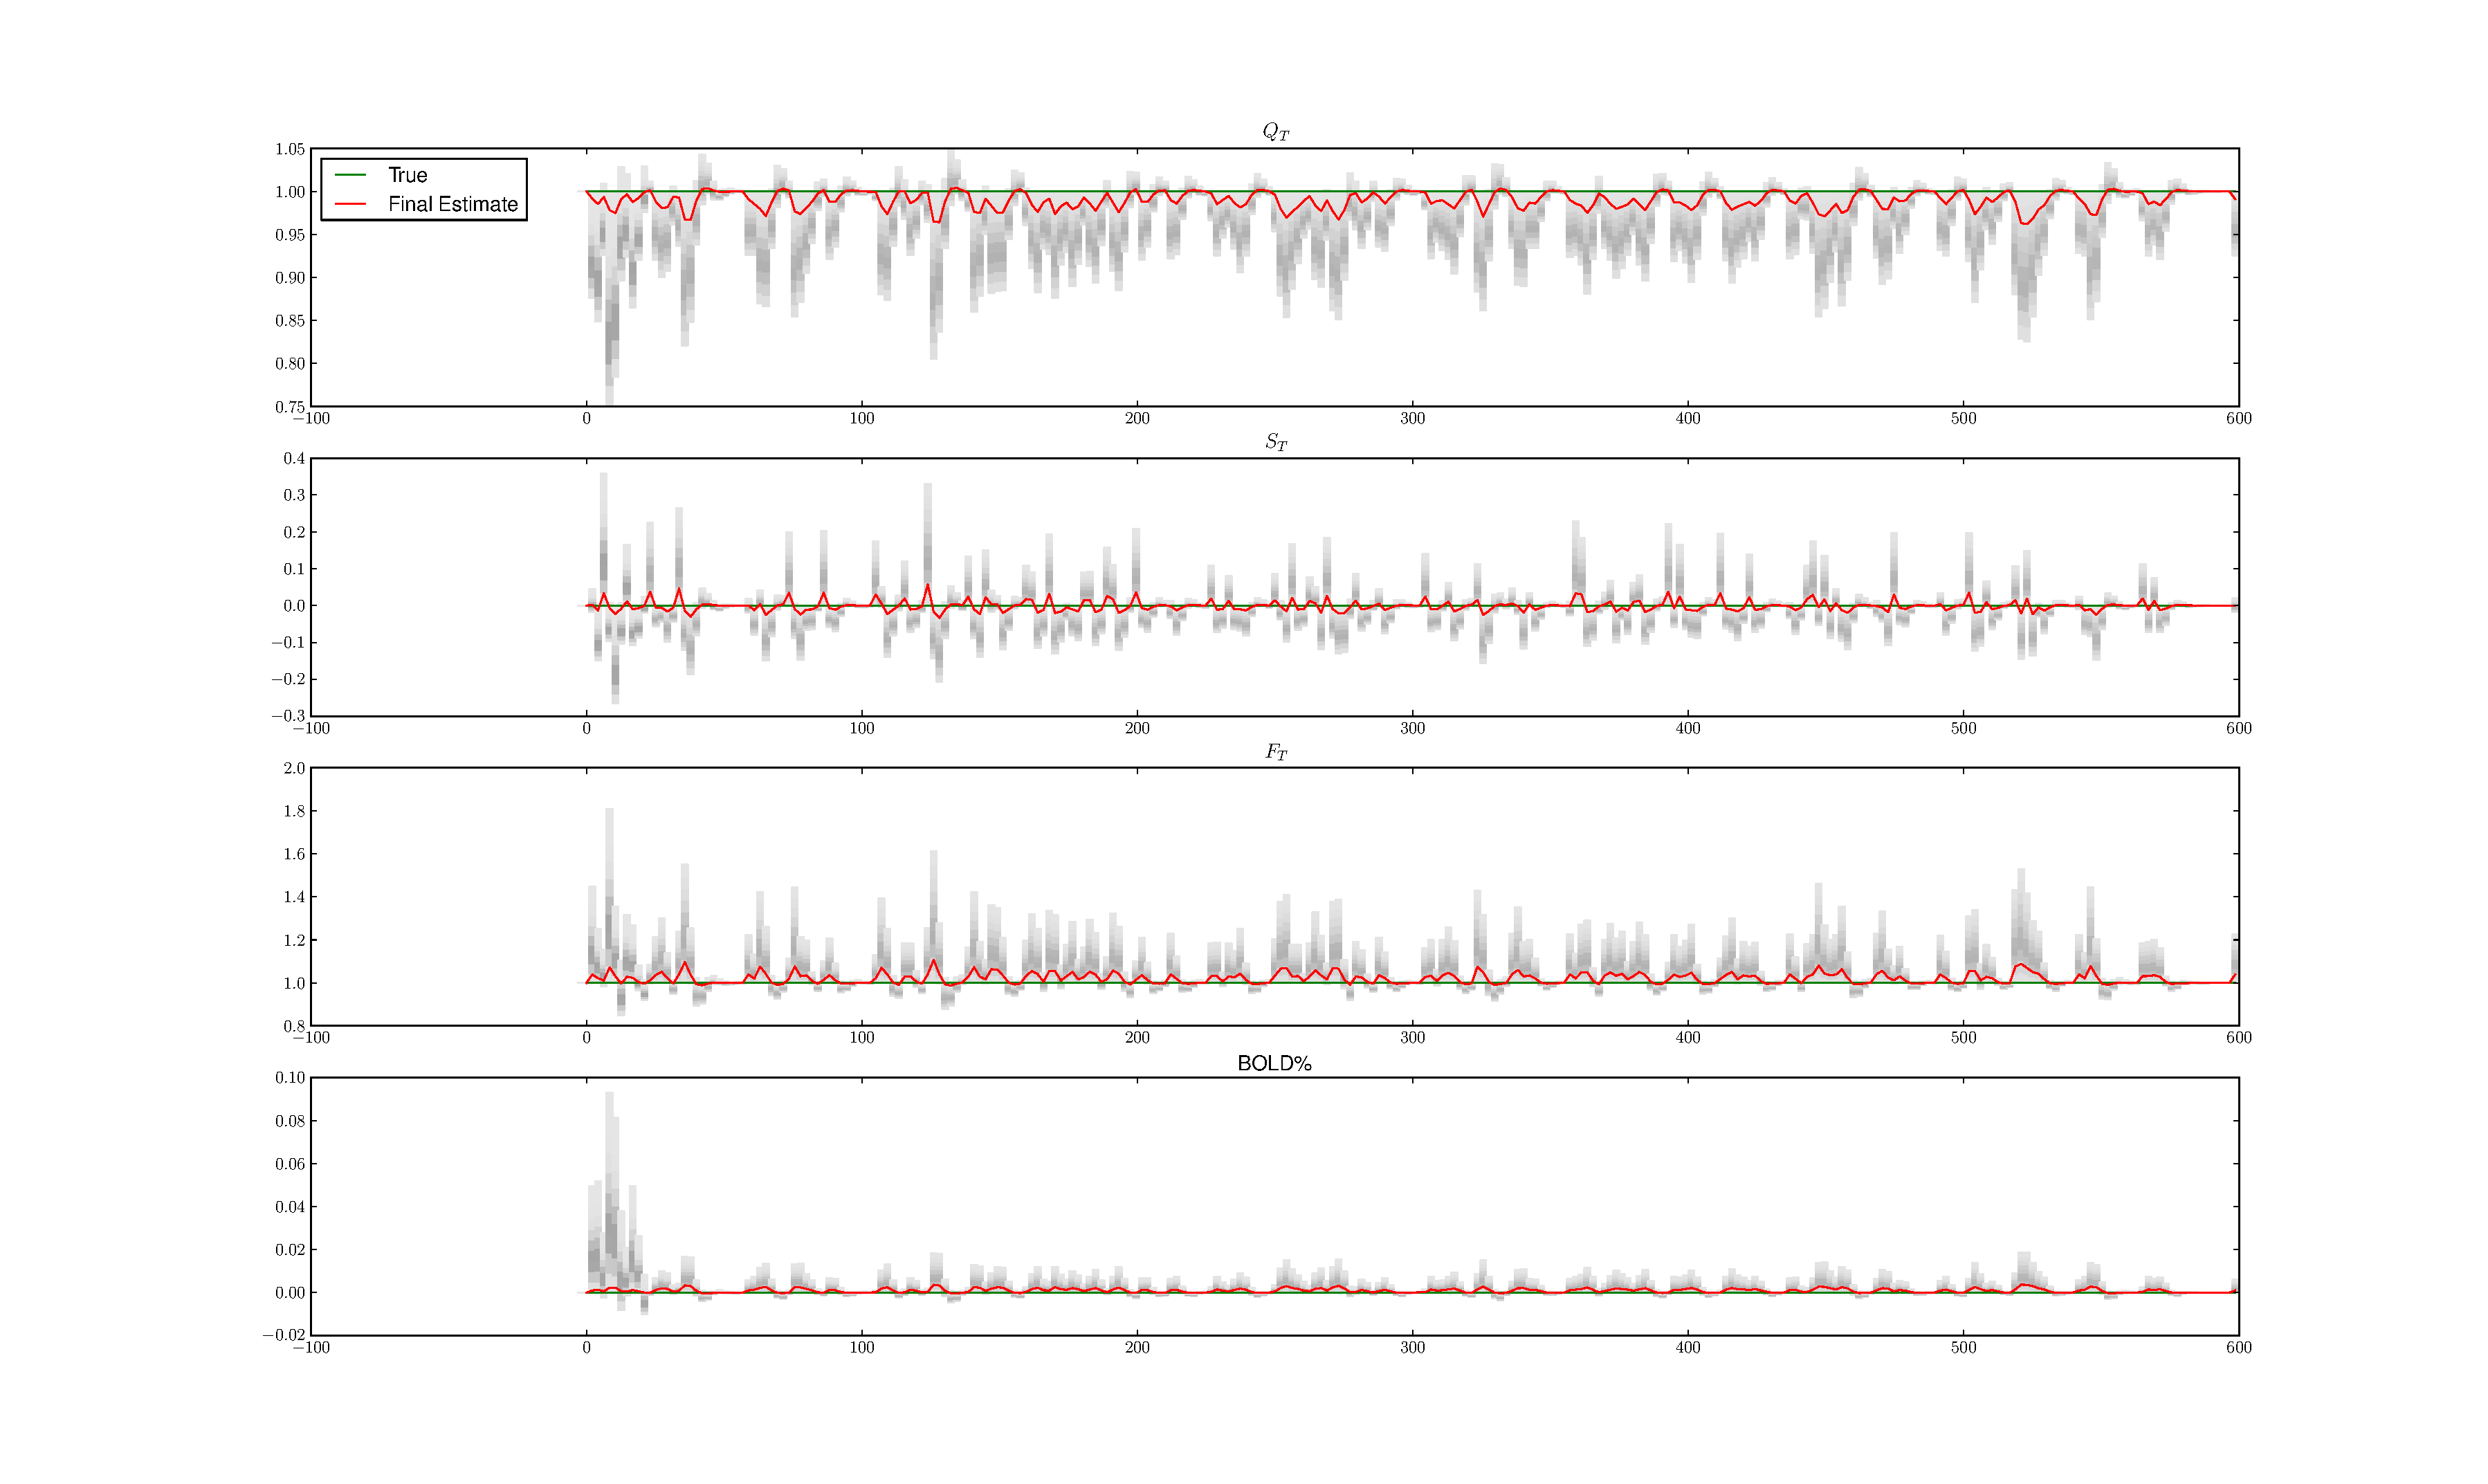
\includegraphics[trim=7cm 3cm 7cm 2cm, width=15cm]{images/justnoise_hist_3}}
\label{fig:JustNoiseConvergence}
\caption{Converging histogram for parameters when the signal consists purely of low level noise. 
Same run as \autoref{fig:justnoise_fit_0}}
\end{figure}

To give a frame of reference to the impulse response level, the impulse response of every
parameter estimated, includeing ones from \autoref{sec:BigNoise}, are shown in \autoref{tab:ImpulseResponses}.


\subsection{Pure Noise, High Magnitude}
\label{sec:PureNoiseHighMag}

\begin{figure}[H]
\label{fig:fits_noiseonly_high}
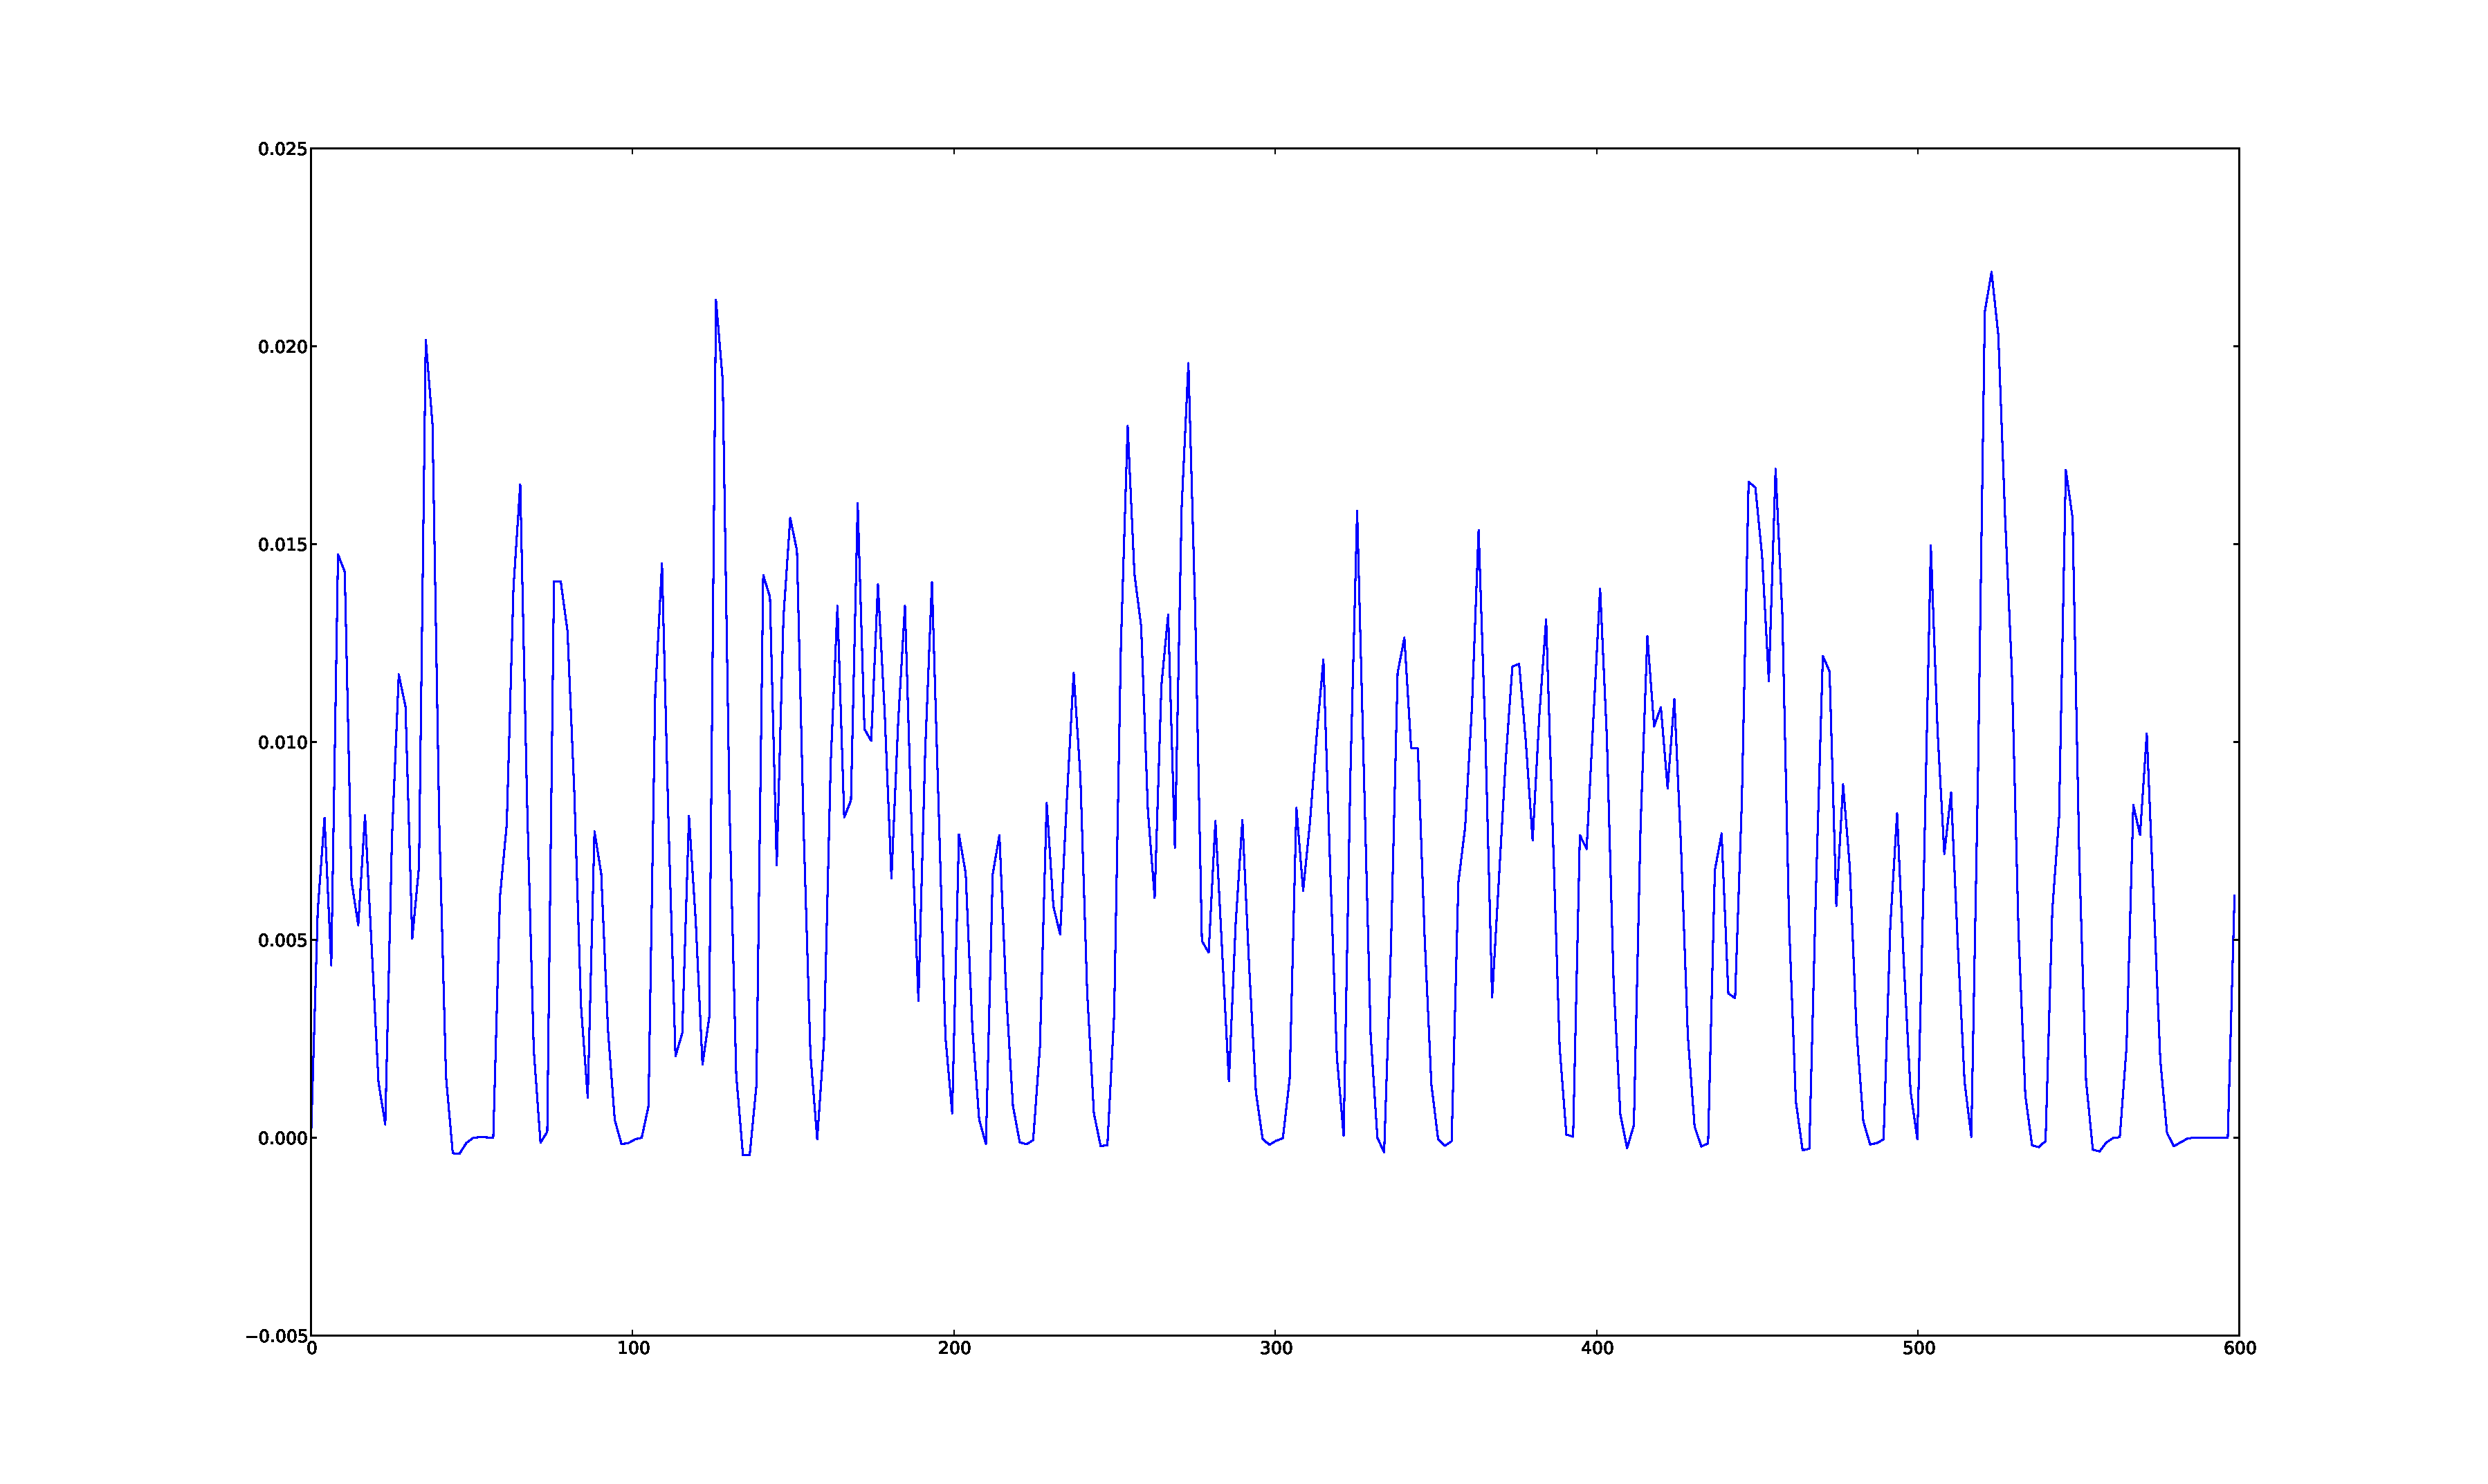
\includegraphics[trim=6cm 3cm 6cm 3cm,width=16cm]{images/fits_noiseonly_high}
\caption{Fits to the non-active, high noise signal. Note that the line is thick because all
the fits overlap. This is all 11 fitted lines.}
\end{figure}

\begin{figure}[H]
\label{fig:justbignoise_fit_0}
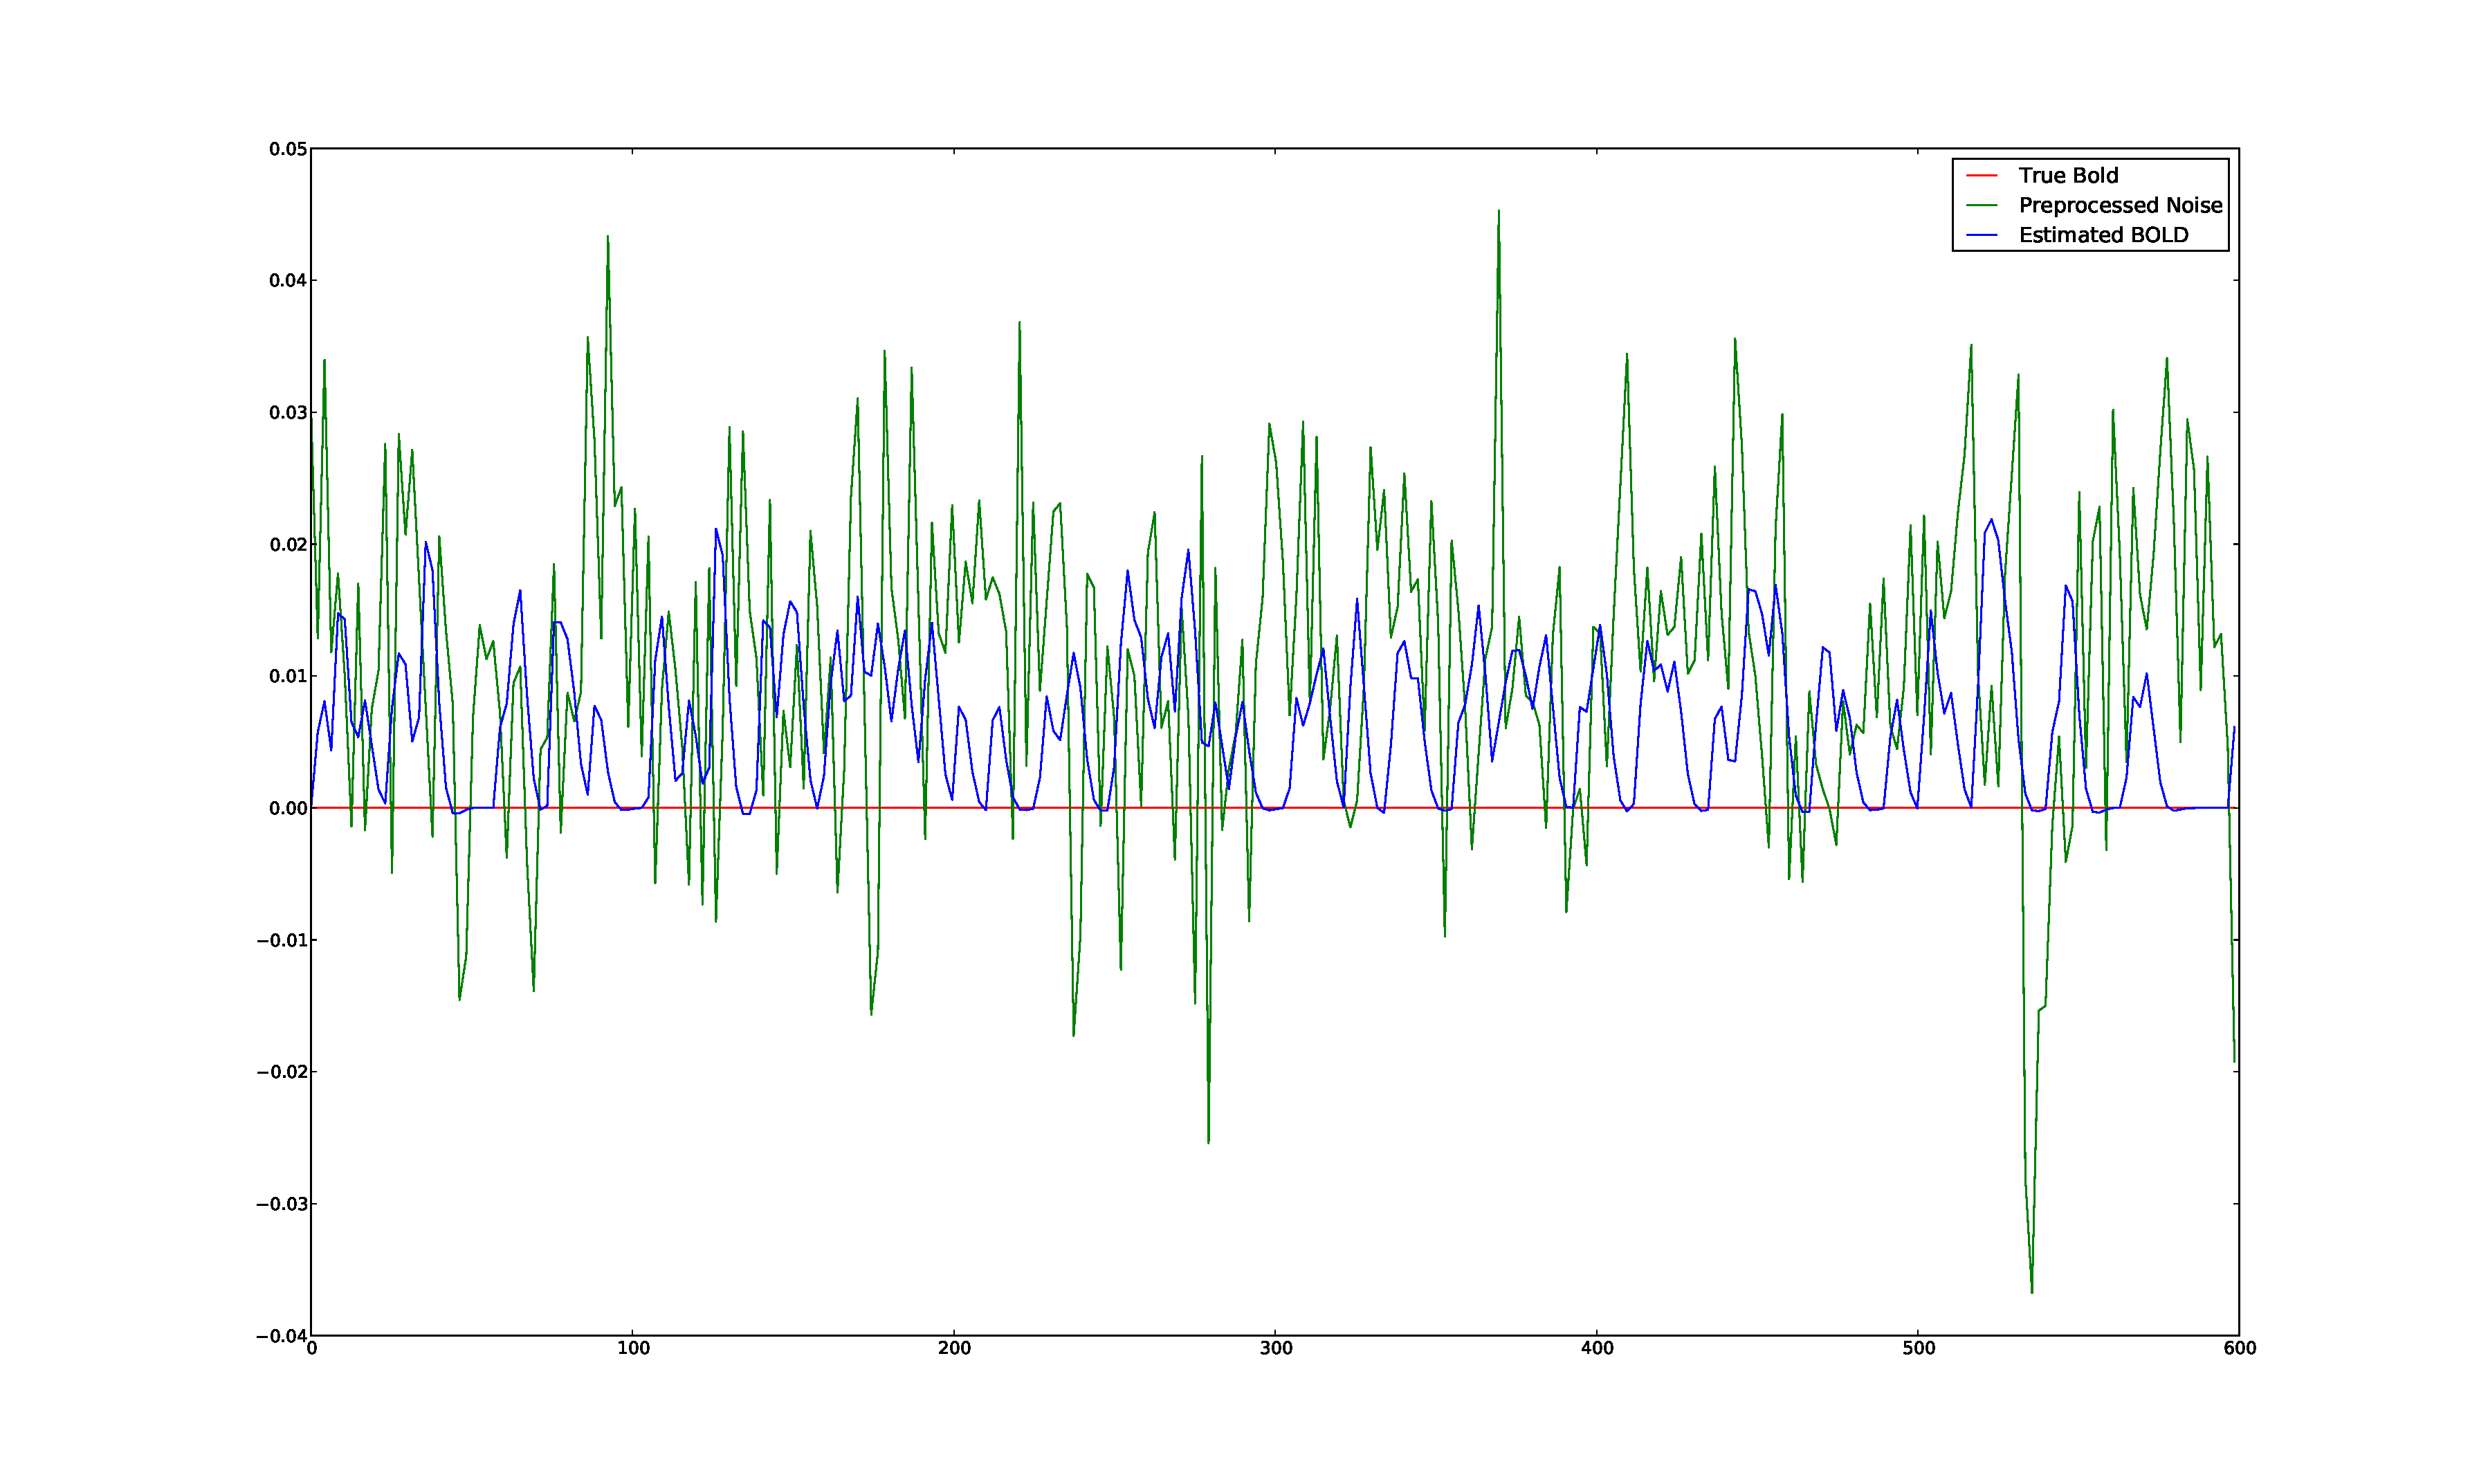
\includegraphics[trim=6cm 3cm 6cm 3cm,width=16cm]{images/justbignoise_fit_0}
\caption{Fit from a single particle filter run, with the noise input. }
\end{figure} %uses allnoise/ALLNOISE-0-w0

\begin{figure}[H]
\subfigure[$\tau_0$, $\alpha$, $E_0$, $V_0$]
{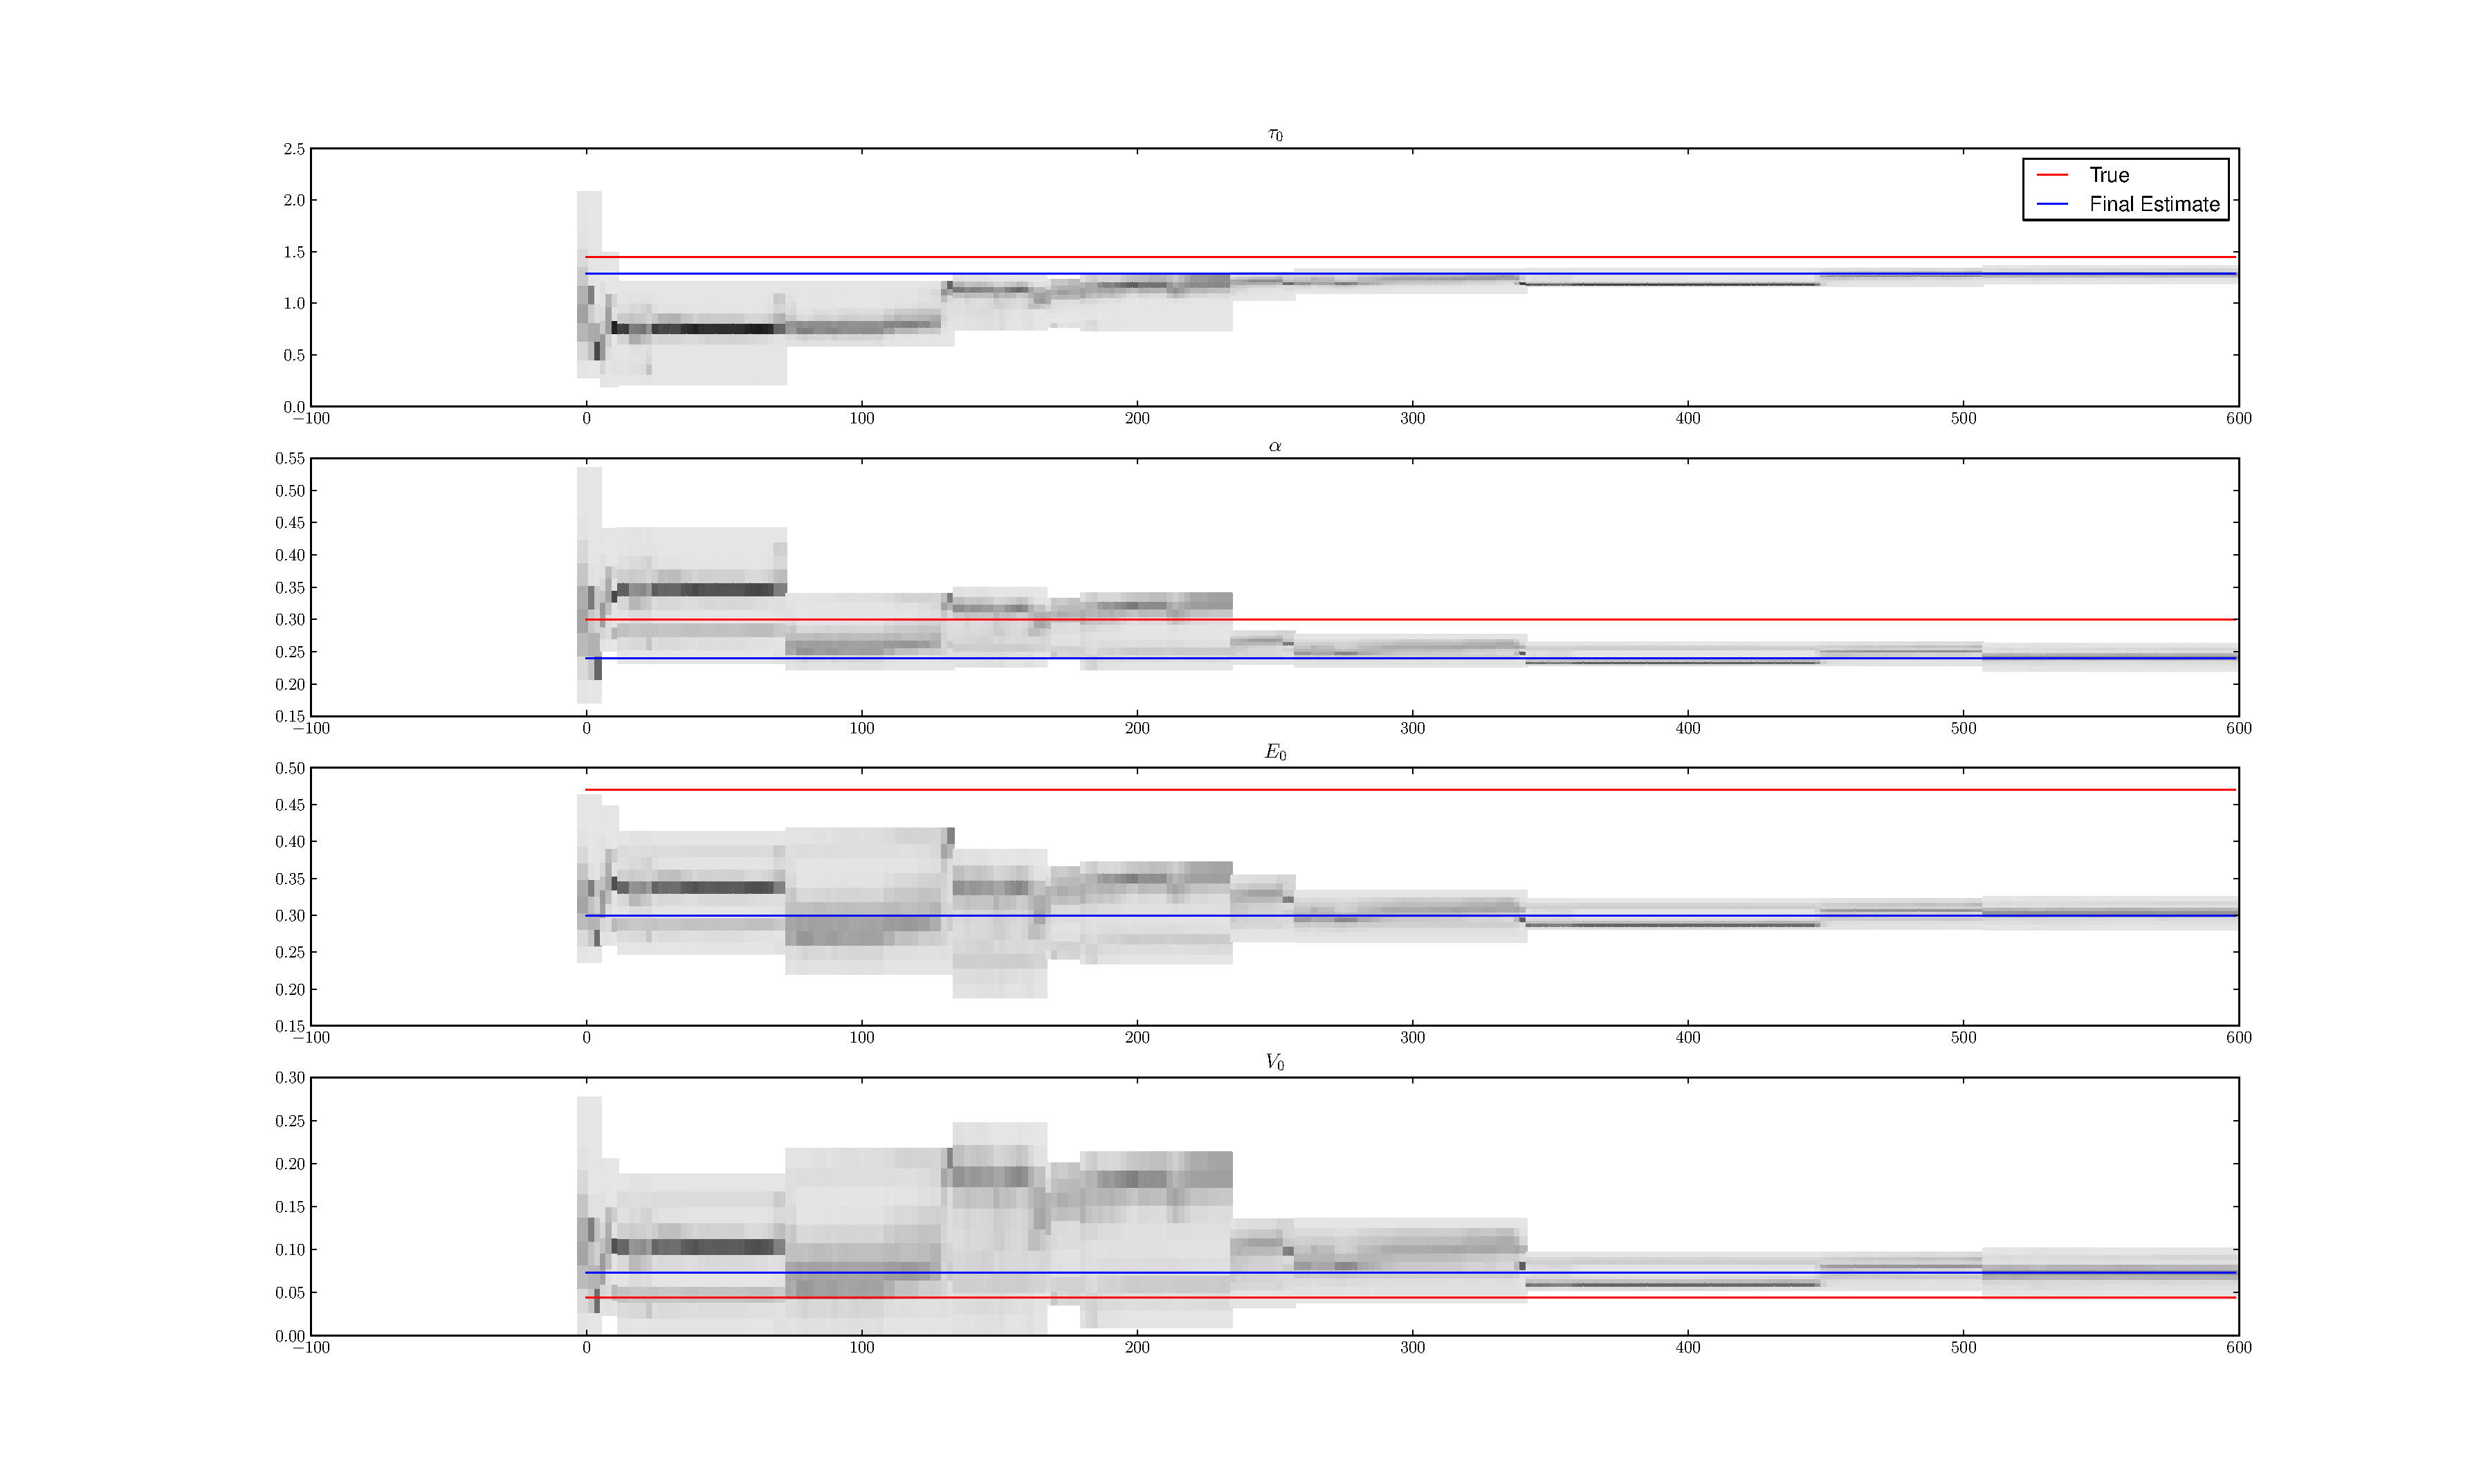
\includegraphics[trim=7cm 3cm 7cm 4cm, width=15cm]{images/justbignoise_1}}\\
\end{figure}
\begin{figure}[H]
\subfigure[$\tau_s$, $\tau_f$, $\epsilon$, $V$] 
{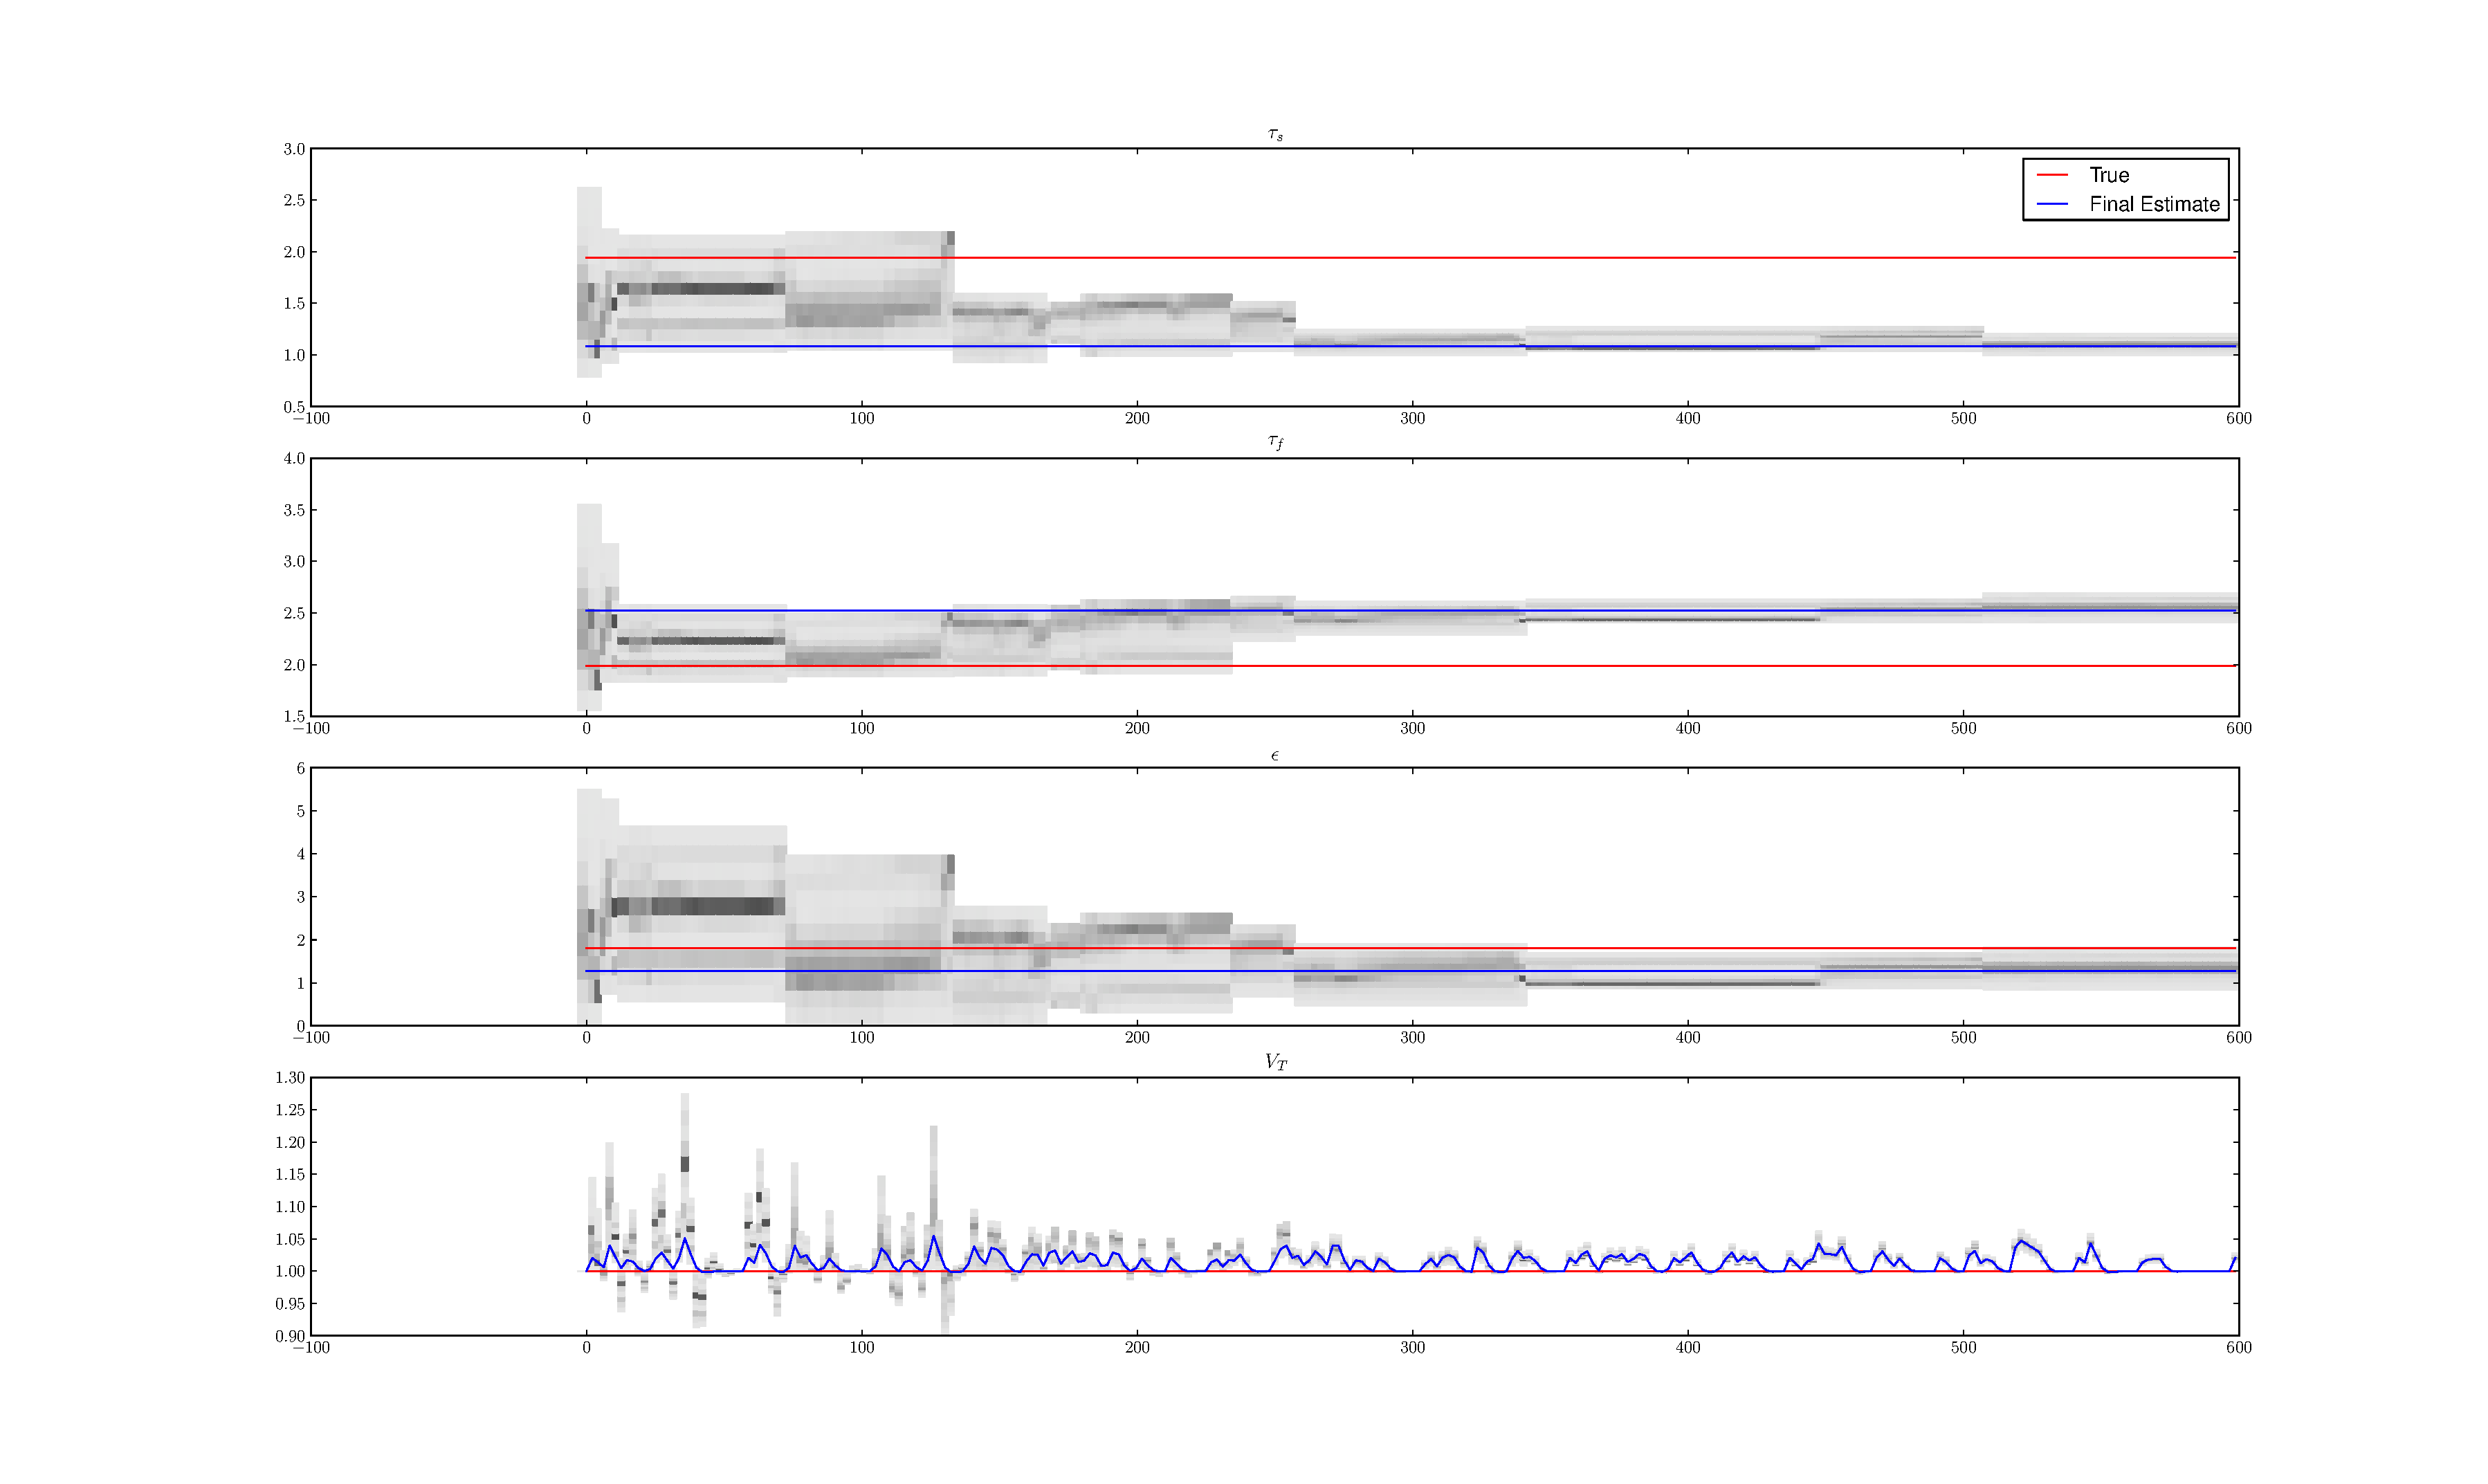
\includegraphics[trim=7cm 3cm 7cm 1cm, width=15cm]{images/justbignoise_2}}\\
\end{figure}
\begin{figure}[H]
\subfigure[$Q$, $S$, $F$, $BOLD$ ]
{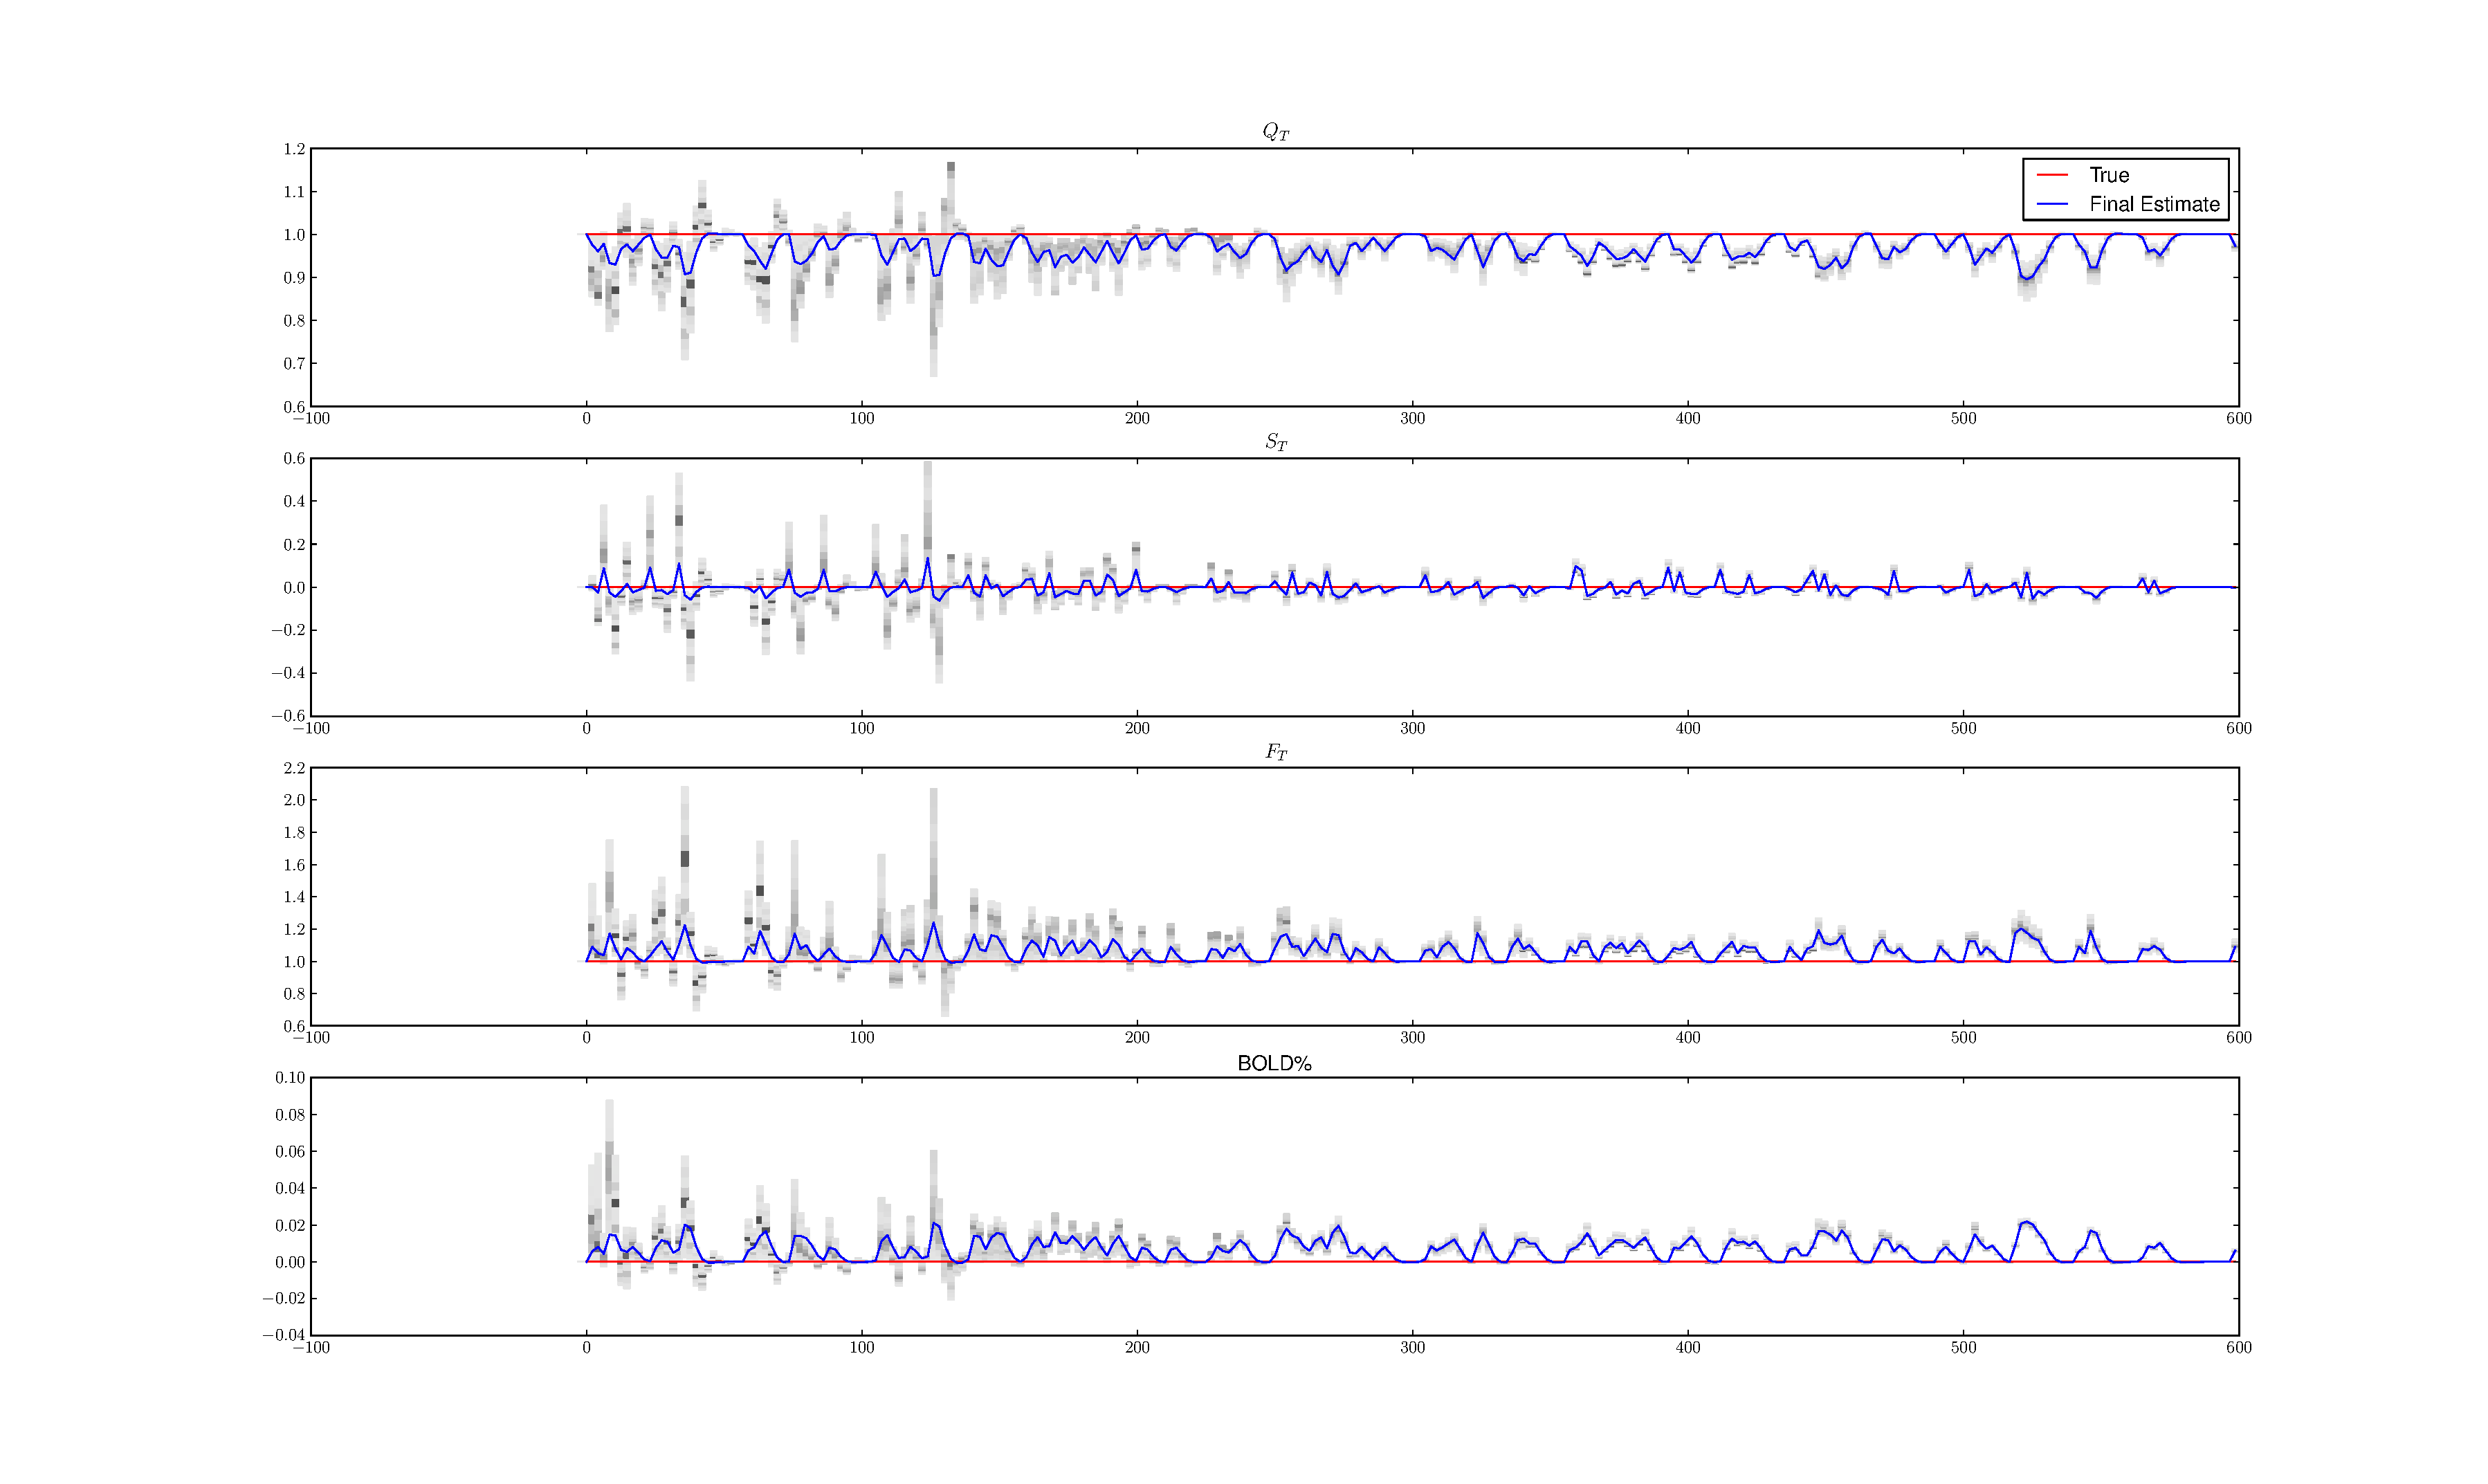
\includegraphics[trim=7cm 3cm 7cm 2cm, width=15cm]{images/justbignoise_3}}
\label{fig:JustNoiseConvergenceLarge}
\caption{Converging histogram for parameters when the signal consists purely of noise, with peaks comparable  to 
the convential BOLD signal. ($\sigma_y = .01, \sigma_x = .005$). Same run as fit in \autoref{fig:justbignoise_fit_0}}
\end{figure}

\subsection{Single Voxel Review}
\begin{table}[t]
\centering
\begin{tabular}{|c | c | c | c | c | c | c | c | c |}
\hline 
& \multicolumn{4}{|c|}{Signal} & \multicolumn{4}{|c|}{No Signal}\\
\hline
& \multicolumn{2}{|c|}{Low Noise} & \multicolumn{2}{|c|}{High Noise} 
& \multicolumn{2}{|c|}{$\sigma_y = .001, \sigma_x = .0005$} 
& \multicolumn{2}{|c|}{$\sigma_y = .01, \sigma_x = .005$}\\
\hline 
&$\sqrt{MSE}$ & $N\sqrt{MSE}$ &
 $\sqrt{MSE}$ & $N\sqrt{MSE}$ &
 $\sqrt{MSE}$ & $N\sqrt{MSE}$ &
 $\sqrt{MSE}$ & $N\sqrt{MSE}$ \\
\hline       
\hline       
1 & 0.003211 & 0.478015  & 0.014065  & 1.038941    &0.001667 & 1.295007 & 0.015114 & 1.33641 \\
2 & 0.003055 & 0.531771  & 0.013731  & 0.951648  &  0.001586 & 1.301750 & 0.015510 & 1.336667 \\
3 & 0.003289 & 0.545798  & 0.012754 &  0.995392  &  0.001651 & 1.26287 &  0.013957 & 1.159567 \\
4 & 0.002847 & 0.498237  & 0.016726  & 1.161286  &  0.001506 & 1.431959 & 0.013814 & 1.099876 \\
5 & 0.003006 & 0.468048  & 0.013698 &  1.039724   & 0.001515 & 1.256645 & 0.014350 & 1.201072 \\
6 & 0.002833 & 0.459001  & 0.011495 &  1.002143  &  0.001557 & 1.270797 & 0.013504 & 1.045886 \\
7 & 0.003028 & 0.460962  & 0.015550 &  1.088472   & 0.001585 & 1.154406 & 0.013006 & 1.205429 \\
8 & 0.003044 & 0.518376  & 0.012054 &  1.059620  &  0.001643 & 1.274564 & 0.015446 & 1.122502 \\
9 & 0.003345 & 0.525303  & 0.015104 &  1.015703  &  0.001679 & 1.320244 & 0.014847 & 1.086366 \\
10 & 0.003175 &0.492111  & 0.012493  & 1.189964  &  0.001826 & 1.344562 & 0.013125 & 1.221350 \\
11 & 0.002889 &0.490919  & 0.012165 &  0.953676  &  0.001950 & 1.325223 & 0.014457 & 1.117367 \\
\hline
mean & 0.003066 & 0.497140  & 0.013621 &  1.04514   &  0.001651 & 1.294366 & 0.014285 & 1.175681 \\
\hline
\end{tabular}
\caption{$\sqrt{MSE}$ and the normalized $\sqrt{MSE}$, $\left(\sqrt{MSE}/(\text{Median Absolute Deviation})\right)$  
for different configurations.} \label{tab:SignleVoxelActivationComparison} 
\end{table}

Comparing the results of \autoref{sec:HighNoise} and \autoref{sec:PureNoiseHighMag}, it is
clear that distinguishing between these cases is a difficult prospect. Although
the impulse response, which is determined by the peak response to a very short input,
is is slightly different, there is no reason to believe that a noise distribution
could not get a higher impulse response. The $\sqrt{MSE}$ is also not going to be
able to distinguish between the high-noise case and the no signal case. Therefore, there
is a noise ceiling above which it will be impossible to determine model validity. The fact
that the particle filter is able to get close to the "true" signal is sadly irrelevant.
Ultimately, a threshold well below those shown in the high noise case 
will have to be placed on the error, if any confidence is going to be placed on the results.

Each test took approximately 60 seconds on an 8 core Xeon (specifics?).

\section{Multi-voxel Simulation}
To test the usefullness of the particle filter for Second I used a modified version of the FSL tool 
POSSUM to generate an entire FMRI image from a parameter map. The parameter map was generated
by taking an existing activation map and assigning discrete parameter sets to each region.
The result was a four dimensional (length x width
x height x parameter) image with spatially varying parameters. Possum was then modified
to take a parameter map and generate activation levels depending on the parameters at that
point. The patch for POSSUM will be made available. As an unfortunate side effect of 
not using Possums' original activation scale, I manually added 750 to the total level of
simulated Possum images. This is because the BOLD \% difference levels were in the range
of 50 - 100\% from the base, about 5 times as large as they should have been. Ultimately
this should not have an effect on the parameters (other than perhaps $\epsilon$ and $V_0$). 
For each time-series in the simulated FMRI image, the final \emph{static} parameters were saved
into a parameter map. This parameter map may then be compared to the map used to generate the 
simulated data; additionally a new simulation using the calculated parameters may also be 
generated to test the difference in activation levels between the real parameters and the
estimated ones. Since it is clear that the parameters are not fully orthogonal 
(\cite{Deneux2006}), its possible that two sets of parameters are functionally equivalent,
but have different parameters. This way, an absolute 
quantitative difference between the two parameter sets may be found.

\section{Real Data}
Finally, we also performed inference based on real FMRI data. The scanner we used...
%... more specifics...

Before performing tests on a full image, I tested the results of the particle filter
on regions deemed active and non-active by statistical parametric mapping. 
\section{Single-Voxel Simulation}
The results 

\section{Single-Voxel Analysis}
This section discusses the results when the particle filter was
applied on a single voxel. The parameters are the same as
those used later for entire image analysis; however, the results
are more in-depth. 

The run-time for a single voxel depends on the several factors. First, the
overall length of the signal being analyzed. For 1000 measurements it takes
about 10 to 15 minutes. On the other hand, in real circumstances the
length is only around 150 measurements. The number of  integration
can certainly make a large difference, however dropping below 1000 (.001 seconds)
is definitely not recommended. 

For a period I considered 1000 to be a
fine number; however when generating simulated data I found that every once
in a while 1000 was not enough. This is problematic in the actual particle
filter since, given the large number of simultaneous integrations taking 
place, its likely that a few particles will fail and be weighted at 0 because
of this problem. Additionally, because the typical case where a failure would
occur is at fast moving times/parameters the particles all tend to fail together.
The result is particle deprivation - no particles with non-zero weights remain.
The other possible outcome is that low time constant particles get pruned resulting
in excessively smoothed estimates for the time series'. Its possible that a
kind of stop-gap measure could be put into place; wherein particles that are
about to be set to NaN are integrated again with finer grained steps. However
many times the non-real results don't occur until several time steps after the 
numbers get strange. So for instance, the timestep was too long, allowing 
$f$ to go negative, resulting in extremely large values of $q$. There are many
different ways where this sort of event can occur, and unfortunately sometimes
there is no way to get back to before the state starting going out of control.

Another crucial factor for run time is how long before the first re-sampling 
occurs. Because the prior is represented initially with significantly more
particles, if the model fits very well, or for some reason the effective
number of particles stays high, resampling could take a long time to occur.
When this happens the particles filter can take a factor of 10 longer to run.
However, if the particle count isn't initially set high, there is a much larger
chance of particle deprivation occurring. Since there is no real way to know
how long it will take to resmaple the first time, there is little the 
algorithm can do to fix this (except perhaps forcing resampling after
some period of time). On the other end of the spectrum, if the time
series doesn't match the model at all, particle deprivation will occur extremely
quickly.  The upshot of this is that the particle filter is able to 
identify these sections very quickly, and thus not waste much time there.
The difficulty though, is the regions in between the perfect fit and the
awful fit. If particle deprivation does occur, did it occur randomly to an
activated region or did it occur inevitably because the region doesn't fit.
The reason for having so many initial particles is to give density to the
distribution to make false negatives more rare. Perhaps the correct method
is to still set the initial particles very high, but if for a long time no
resampling occurs, halve the standard deviation of the measurement error.
Thus, if the weighting function is not discriminating enough, force it 
to be more picky about the results. Of course this could lead to particle
deprivation as well if the standard deviation is brought down too quickly.
Of course, if a fat-tailed distribution is used for the weighting function,
or the standard deviation of a Gaussian weighting function is sufficiently large,
the particle filter will simply converge to meaningless values. The question
of whether 

\begin{figure}
\label{fig:badfit}
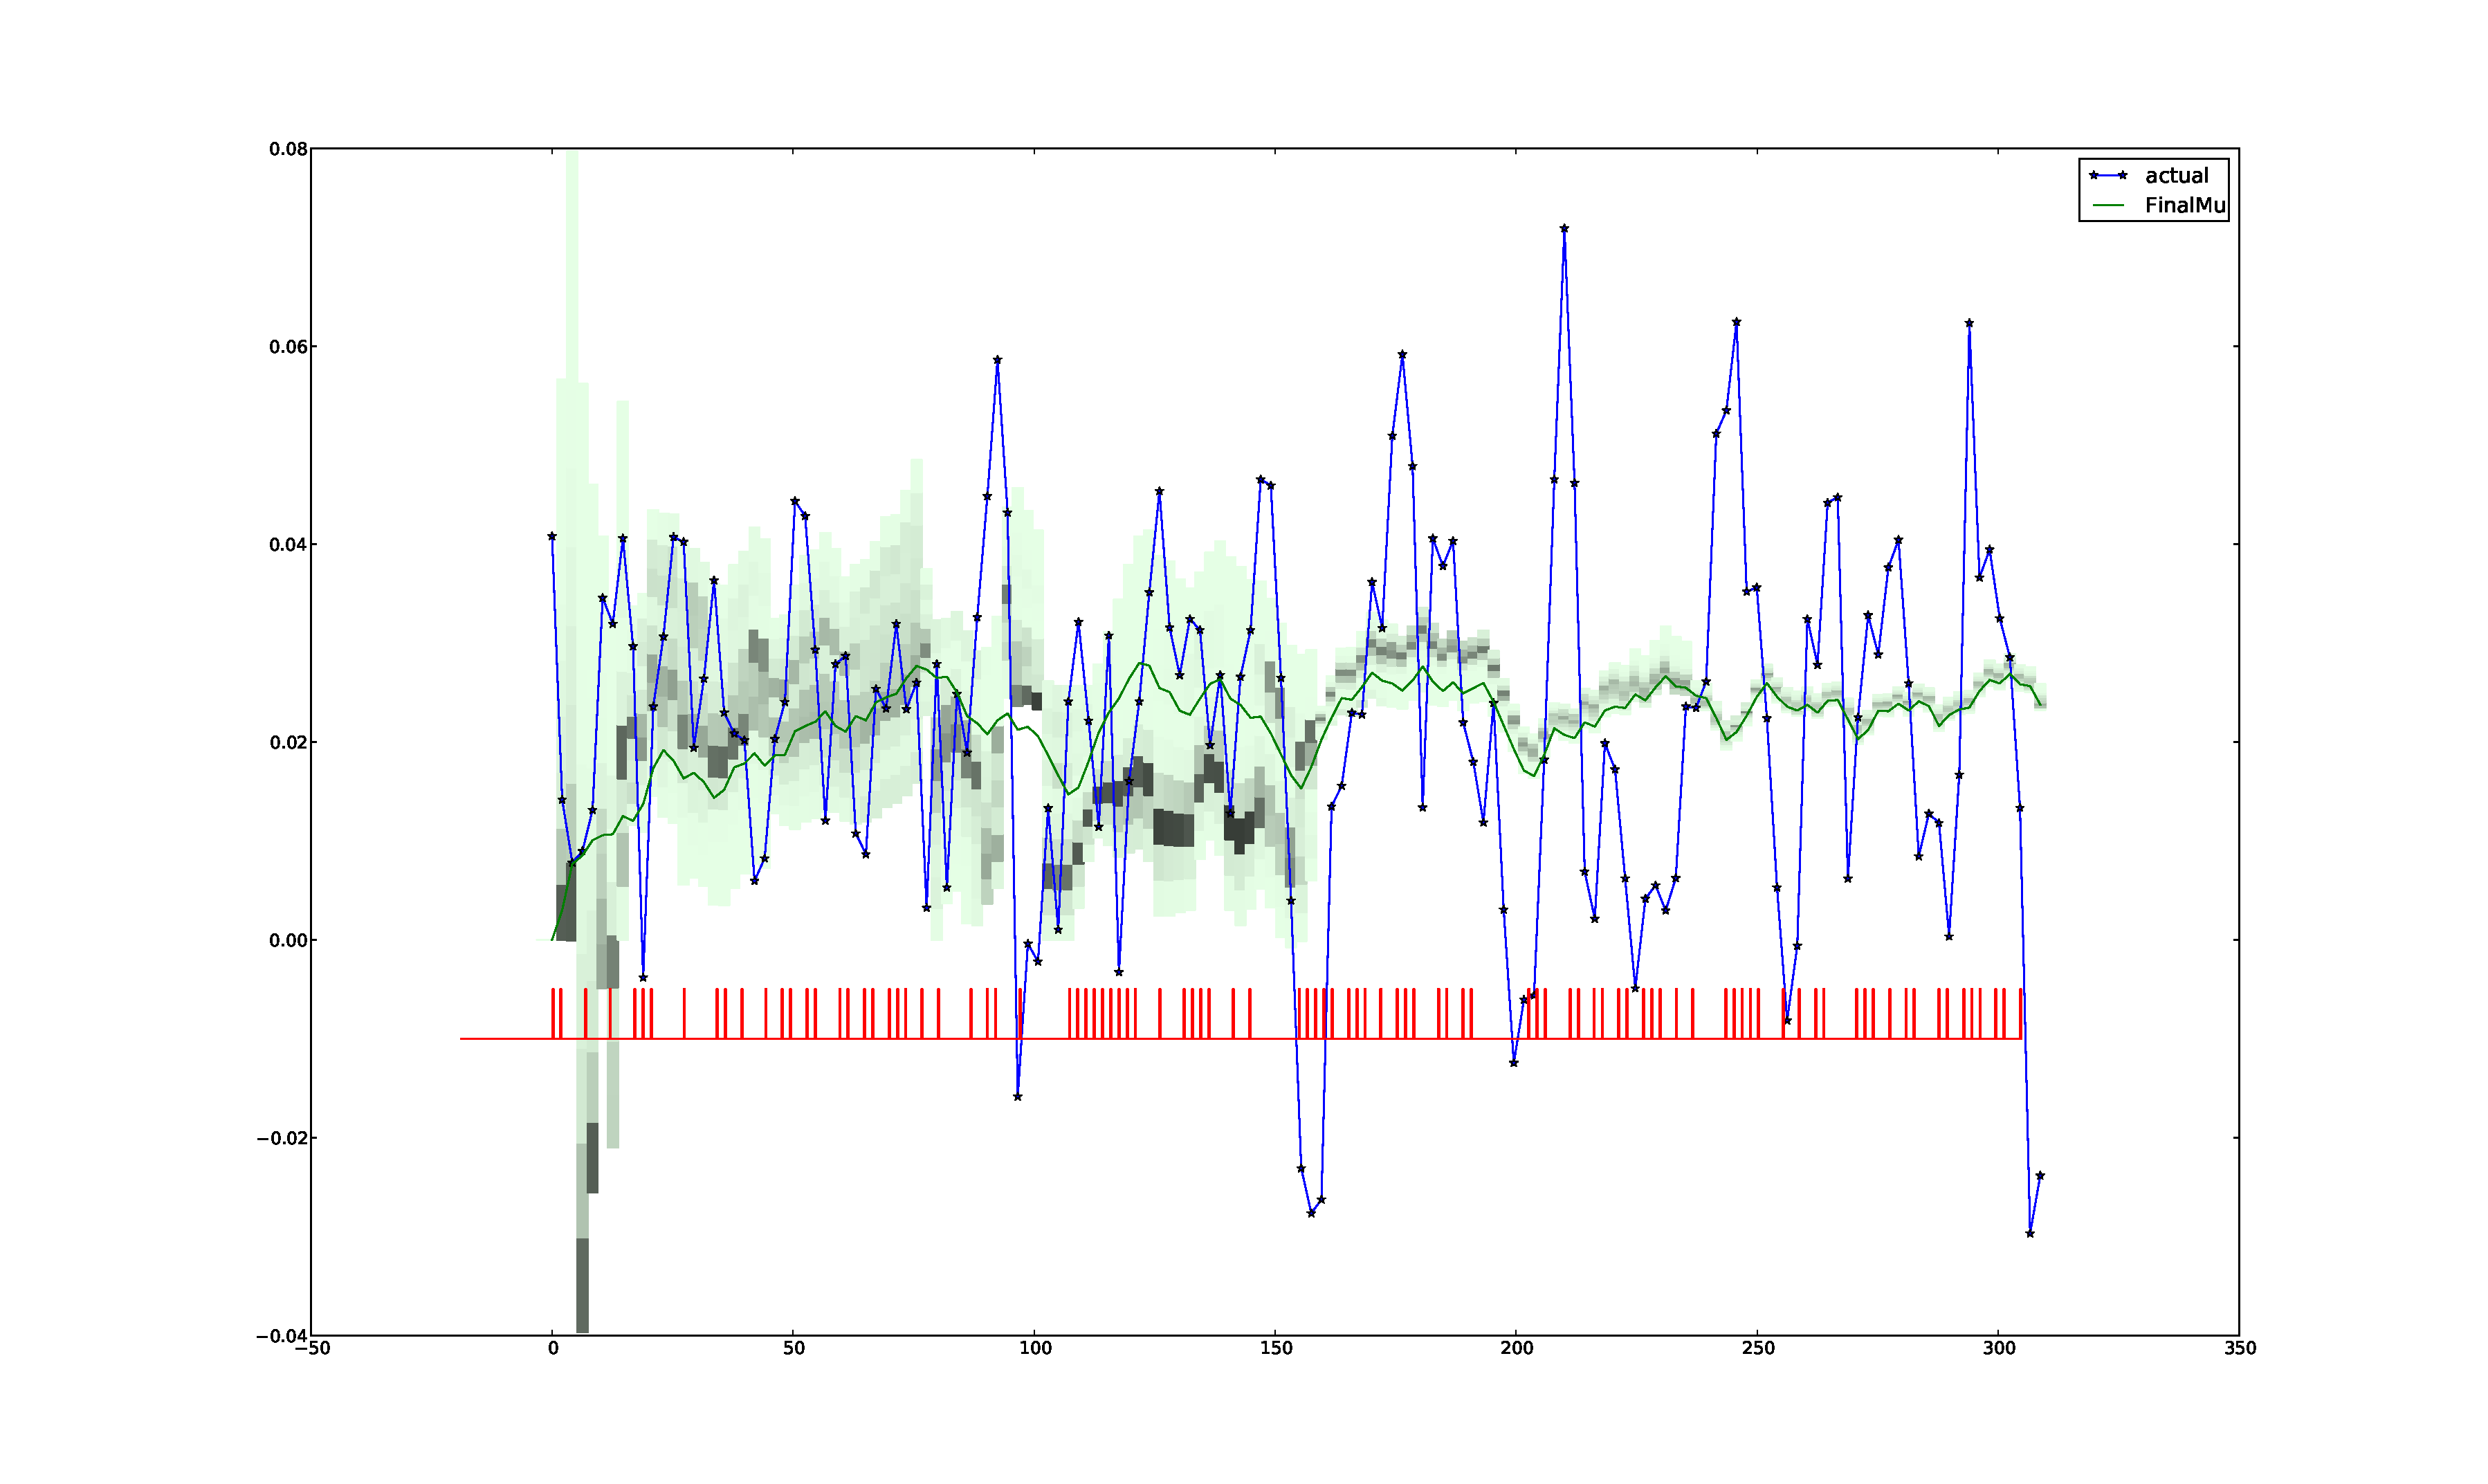
\includegraphics[trim=10cm 4cm 10cm 4cm, width=16cm]{images/inactive_illogical}
\caption{Particle Filter converging to values that make little sense,
because the voxel did not correlate with the input in any known way}
\end{figure}

\begin{figure}
\label{fig:highhard}
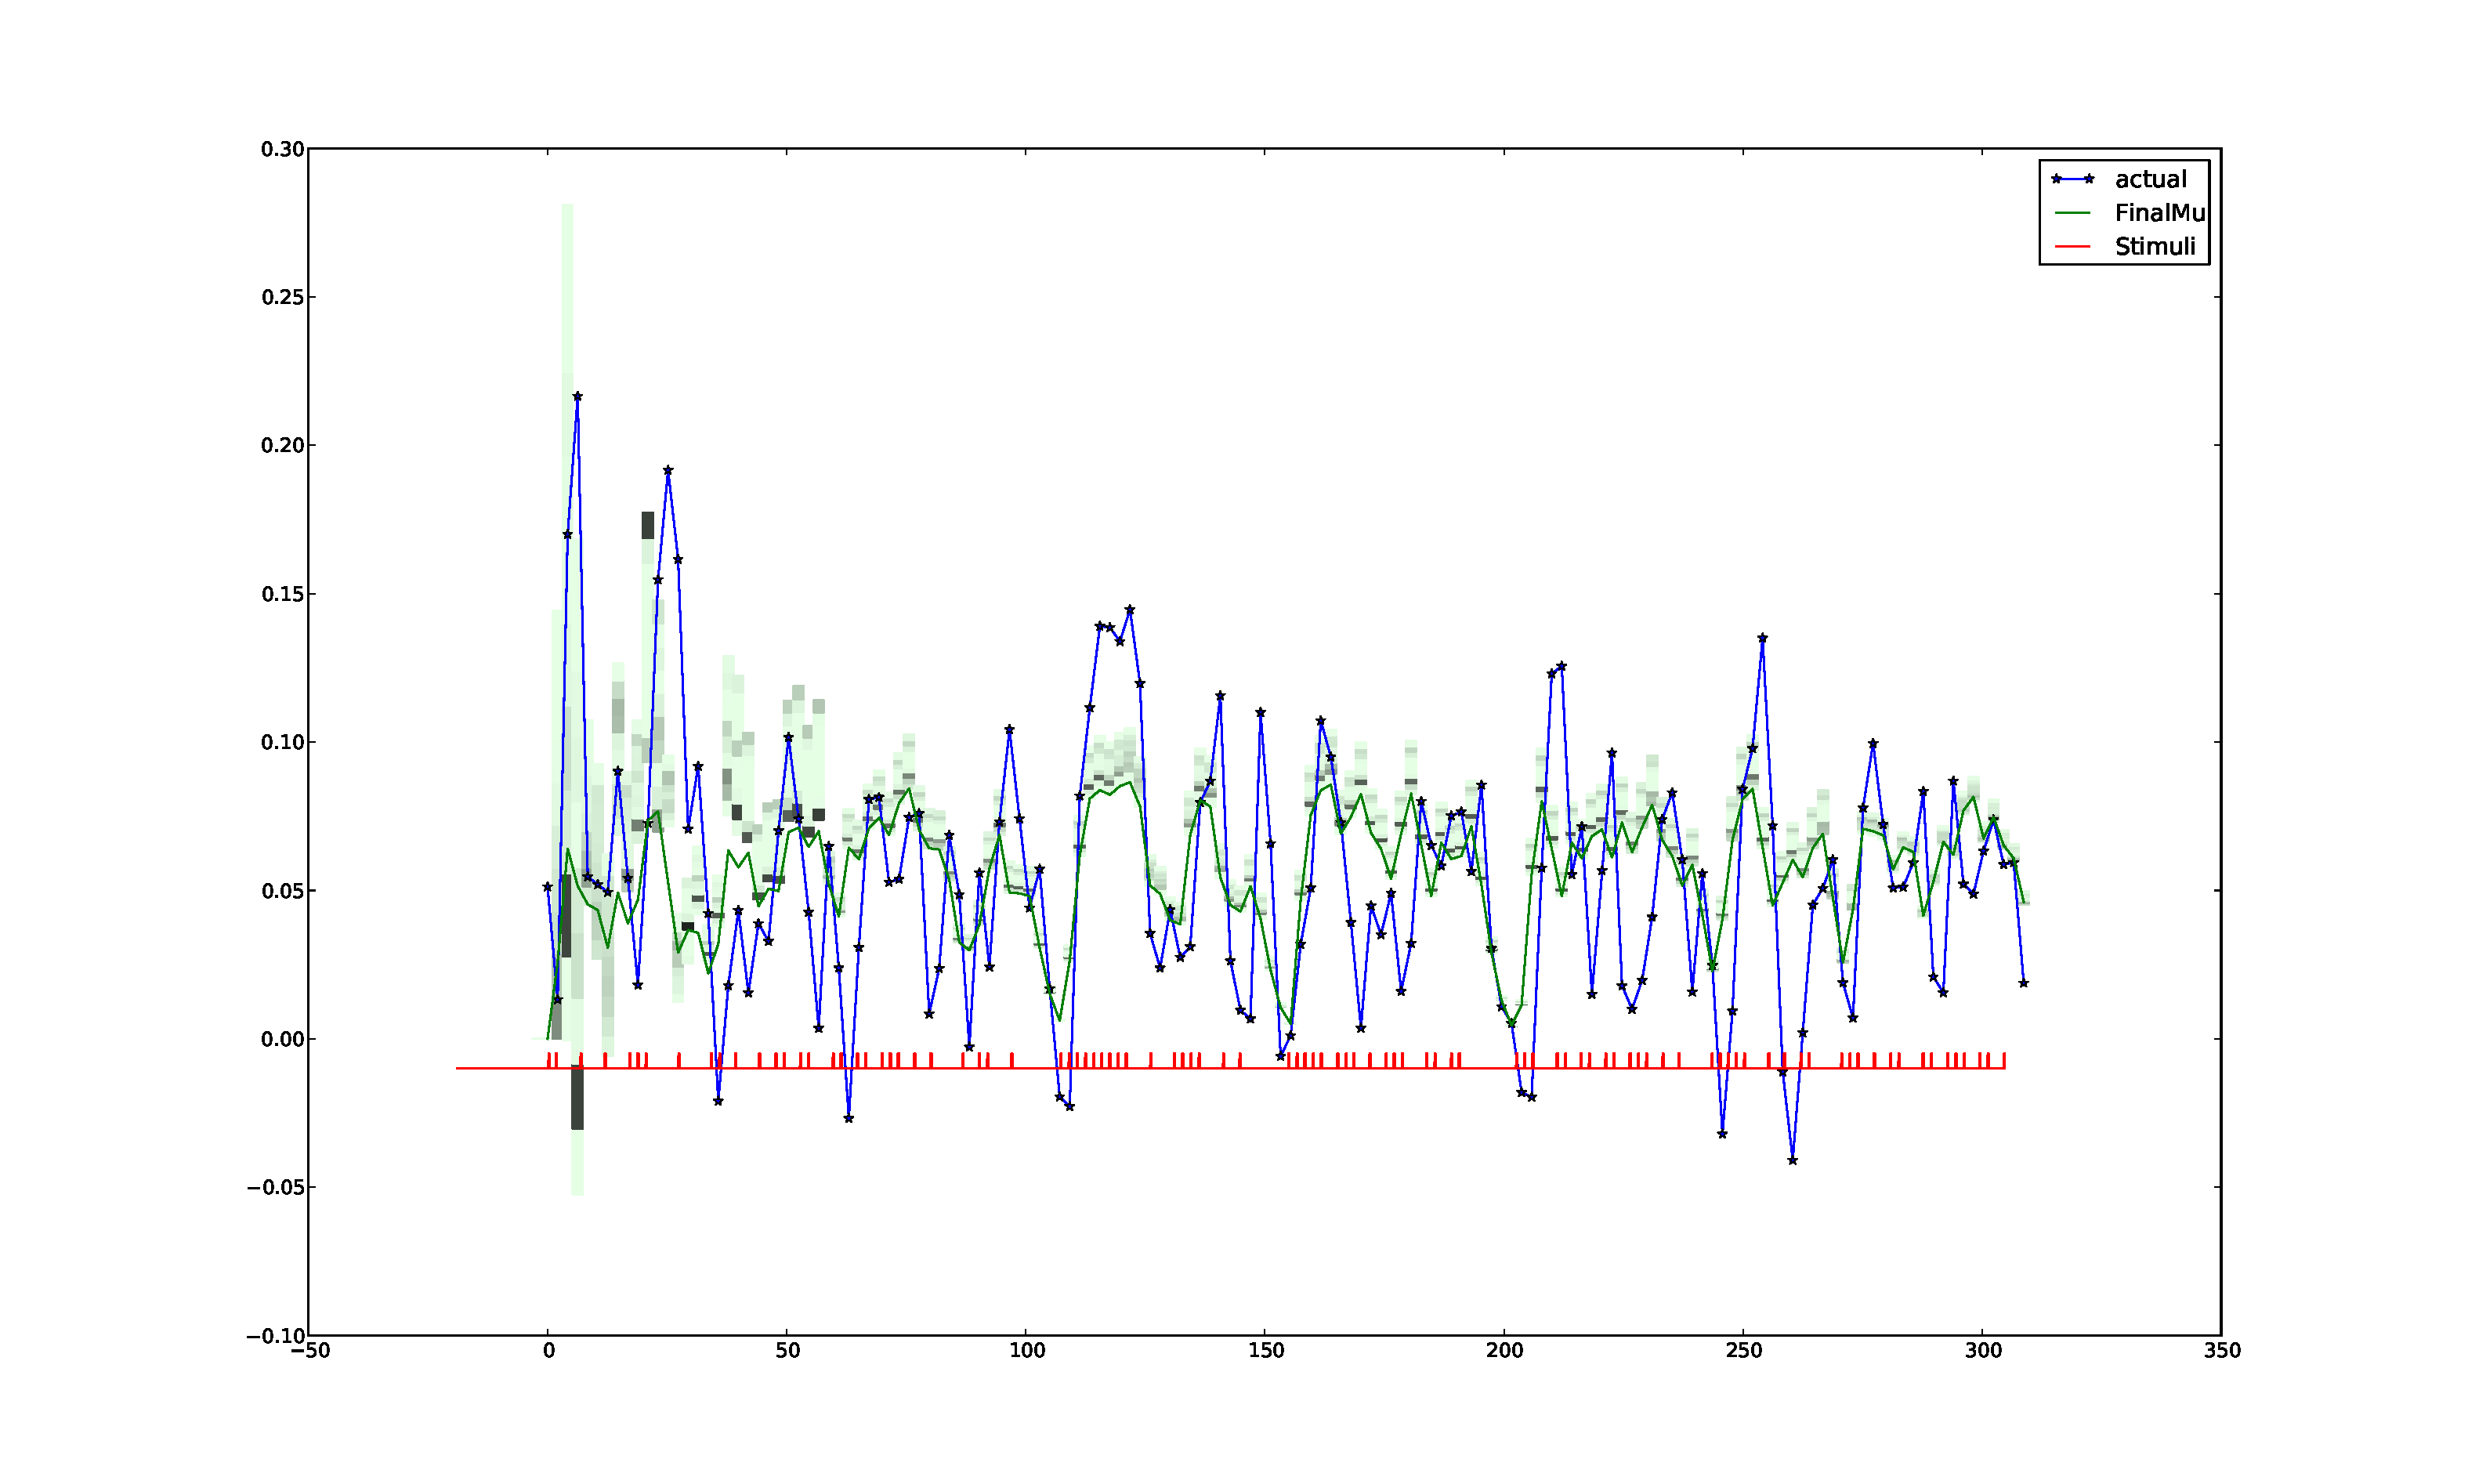
\includegraphics[trim=10cm 4cm 10cm 4cm, width=16cm]{images/active_difficult}
\caption{Example of a timeseries that laplace performs better on than
gaussian. The large spike at the beginning can quickly eliminate all particles} 

\end{figure}

For this reason, it is important to threshold based on the MSE, and the
impulse response. Naturally the MSE is intended to catch very voxels with a
very poor fit,
but like \autoref{fig:badfit}, the algorithm may have found a line
down the middle that gives a decent mean squared error. In this case
the excessive smoothing and low actual activation level will easily
be distinguished by finding the peak response to single short pulse. 

The choice of a prior, as discussed previously, is extremely important. While a
prior may have the potential to give good results, being a monte-carlo algorithm
there is the possibility for inconsistencies. Thus, increasing the variance
of the time-constants may allow additional flexibility, it will also cause
additional model variance. Case in point, the exact same algorithm run twice
with standard deviations of $.35, .35, .35$ for the time constants resulted in two
very different fits, see \autoref{fig:param1_var}.

\begin{figure}
\label{fig:badfit_param1}
\subfigure[]{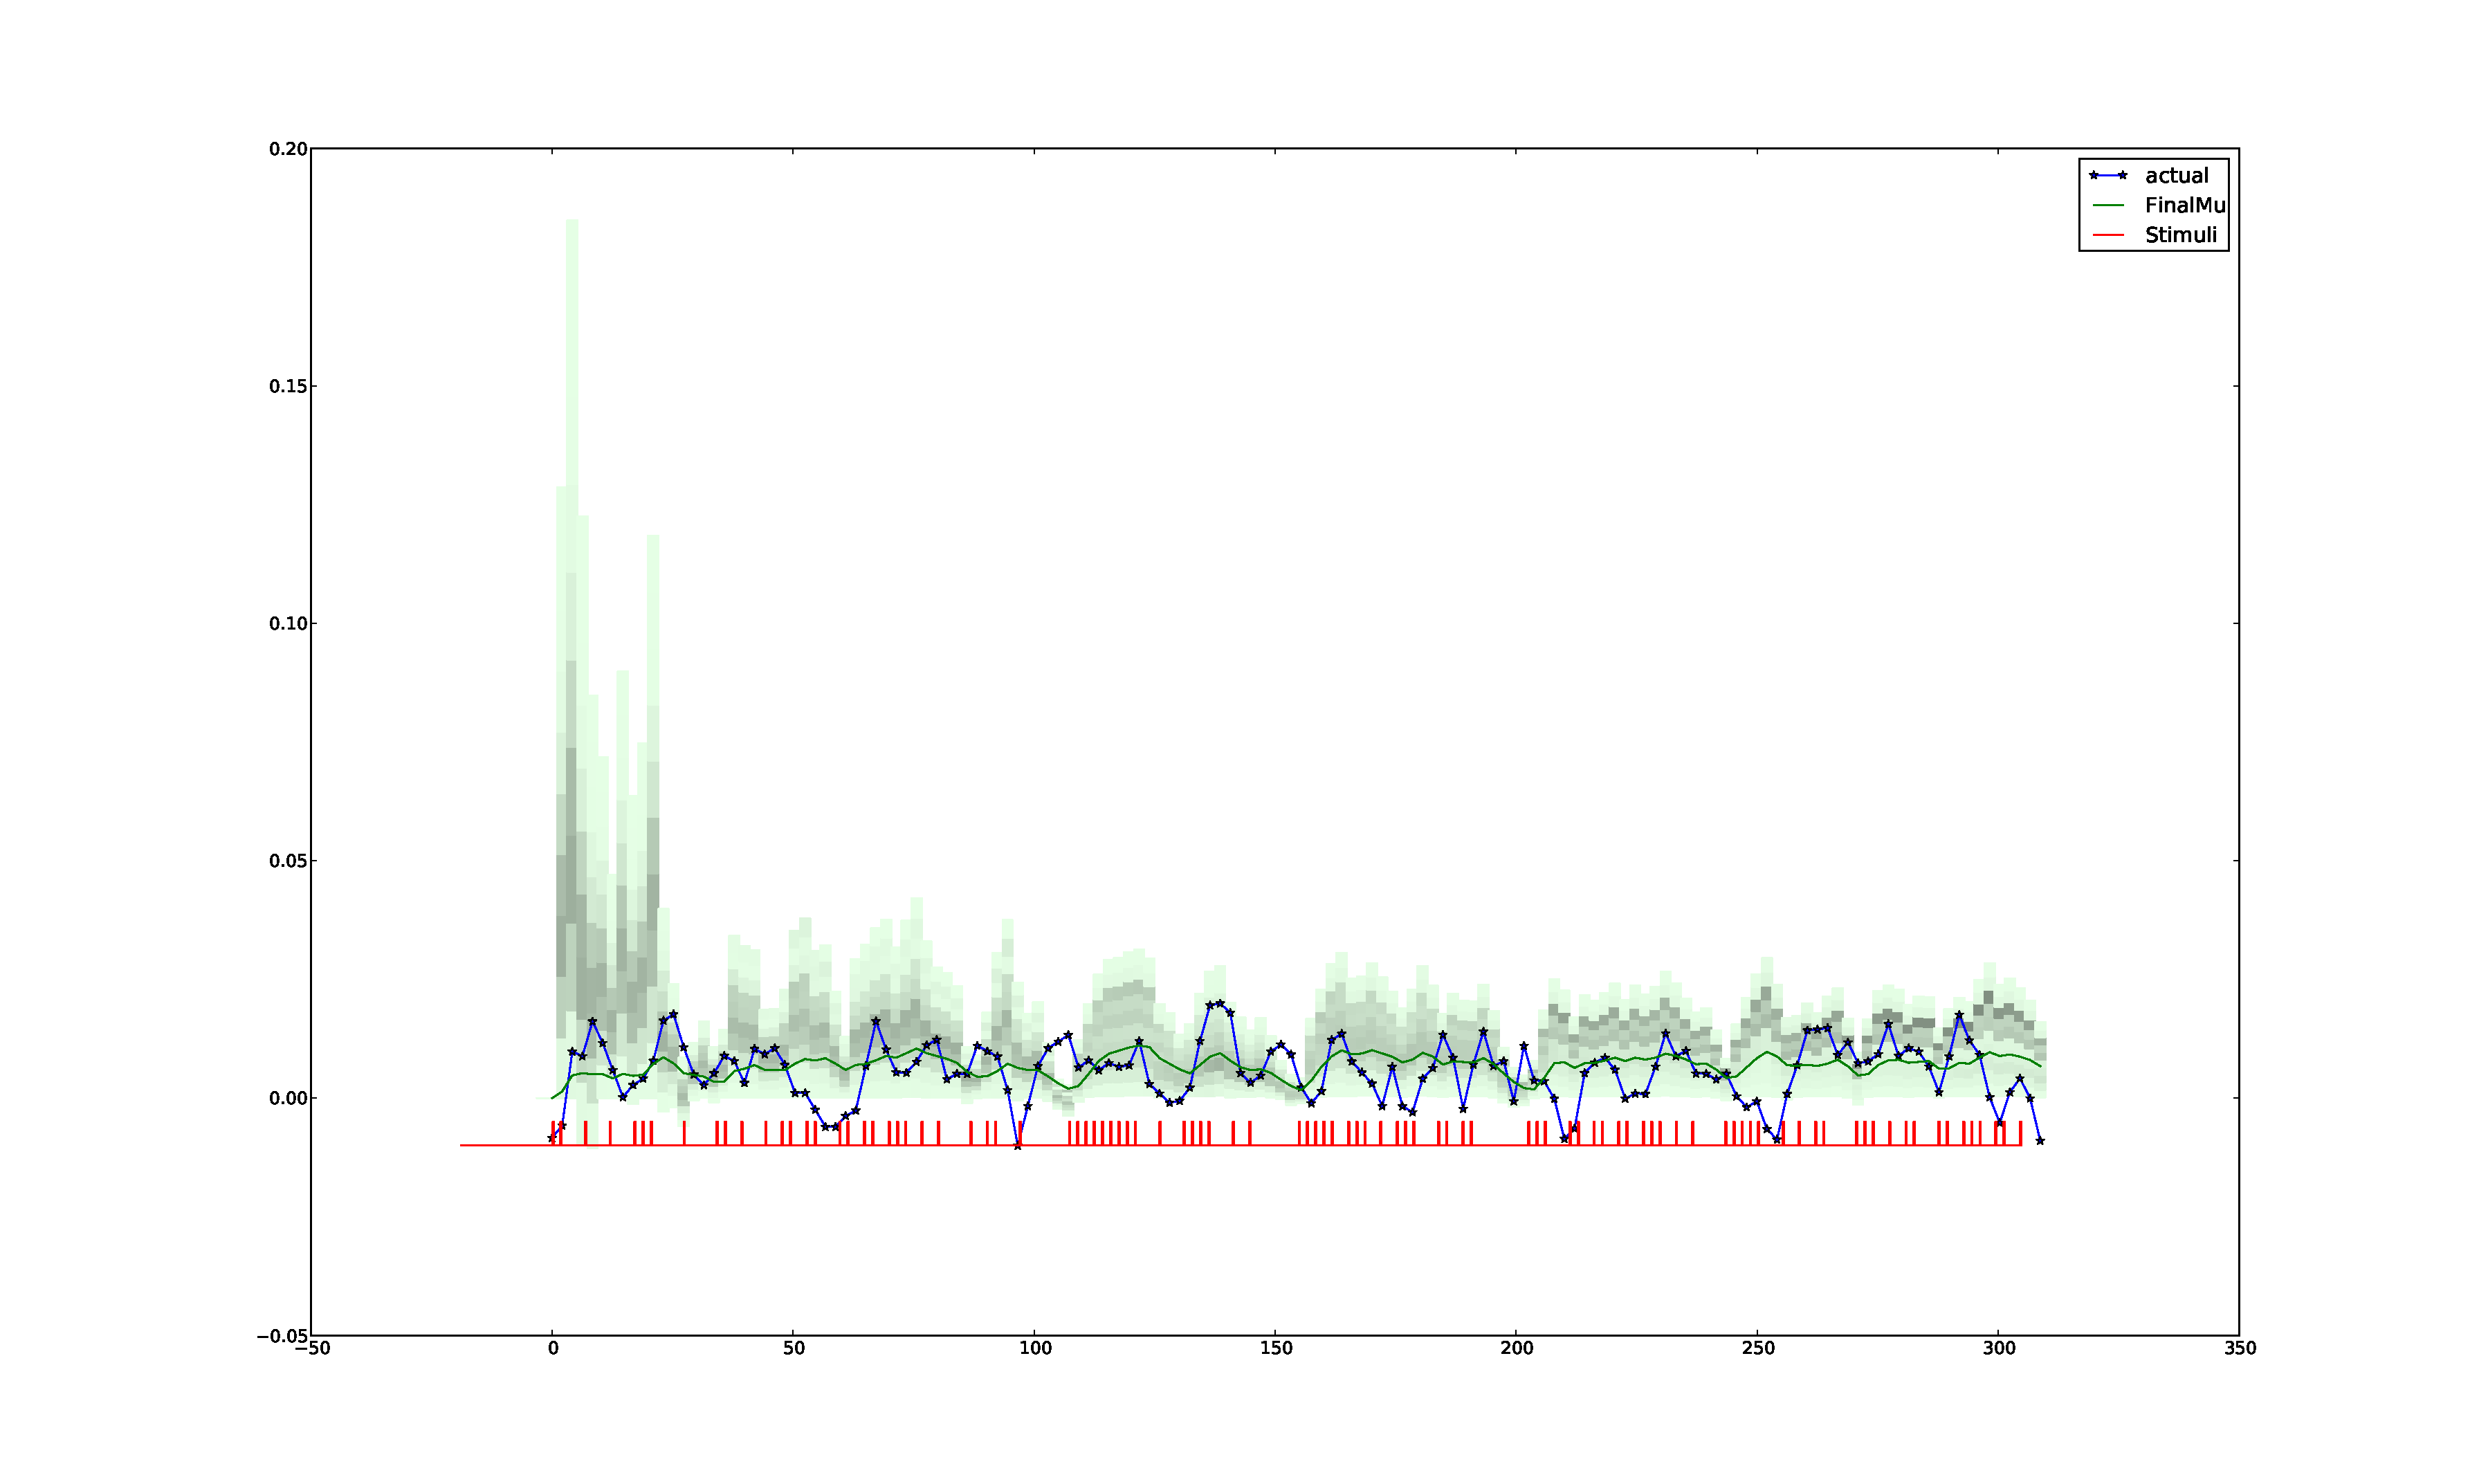
\includegraphics{images/badfit_param1}}
\subfigure[]{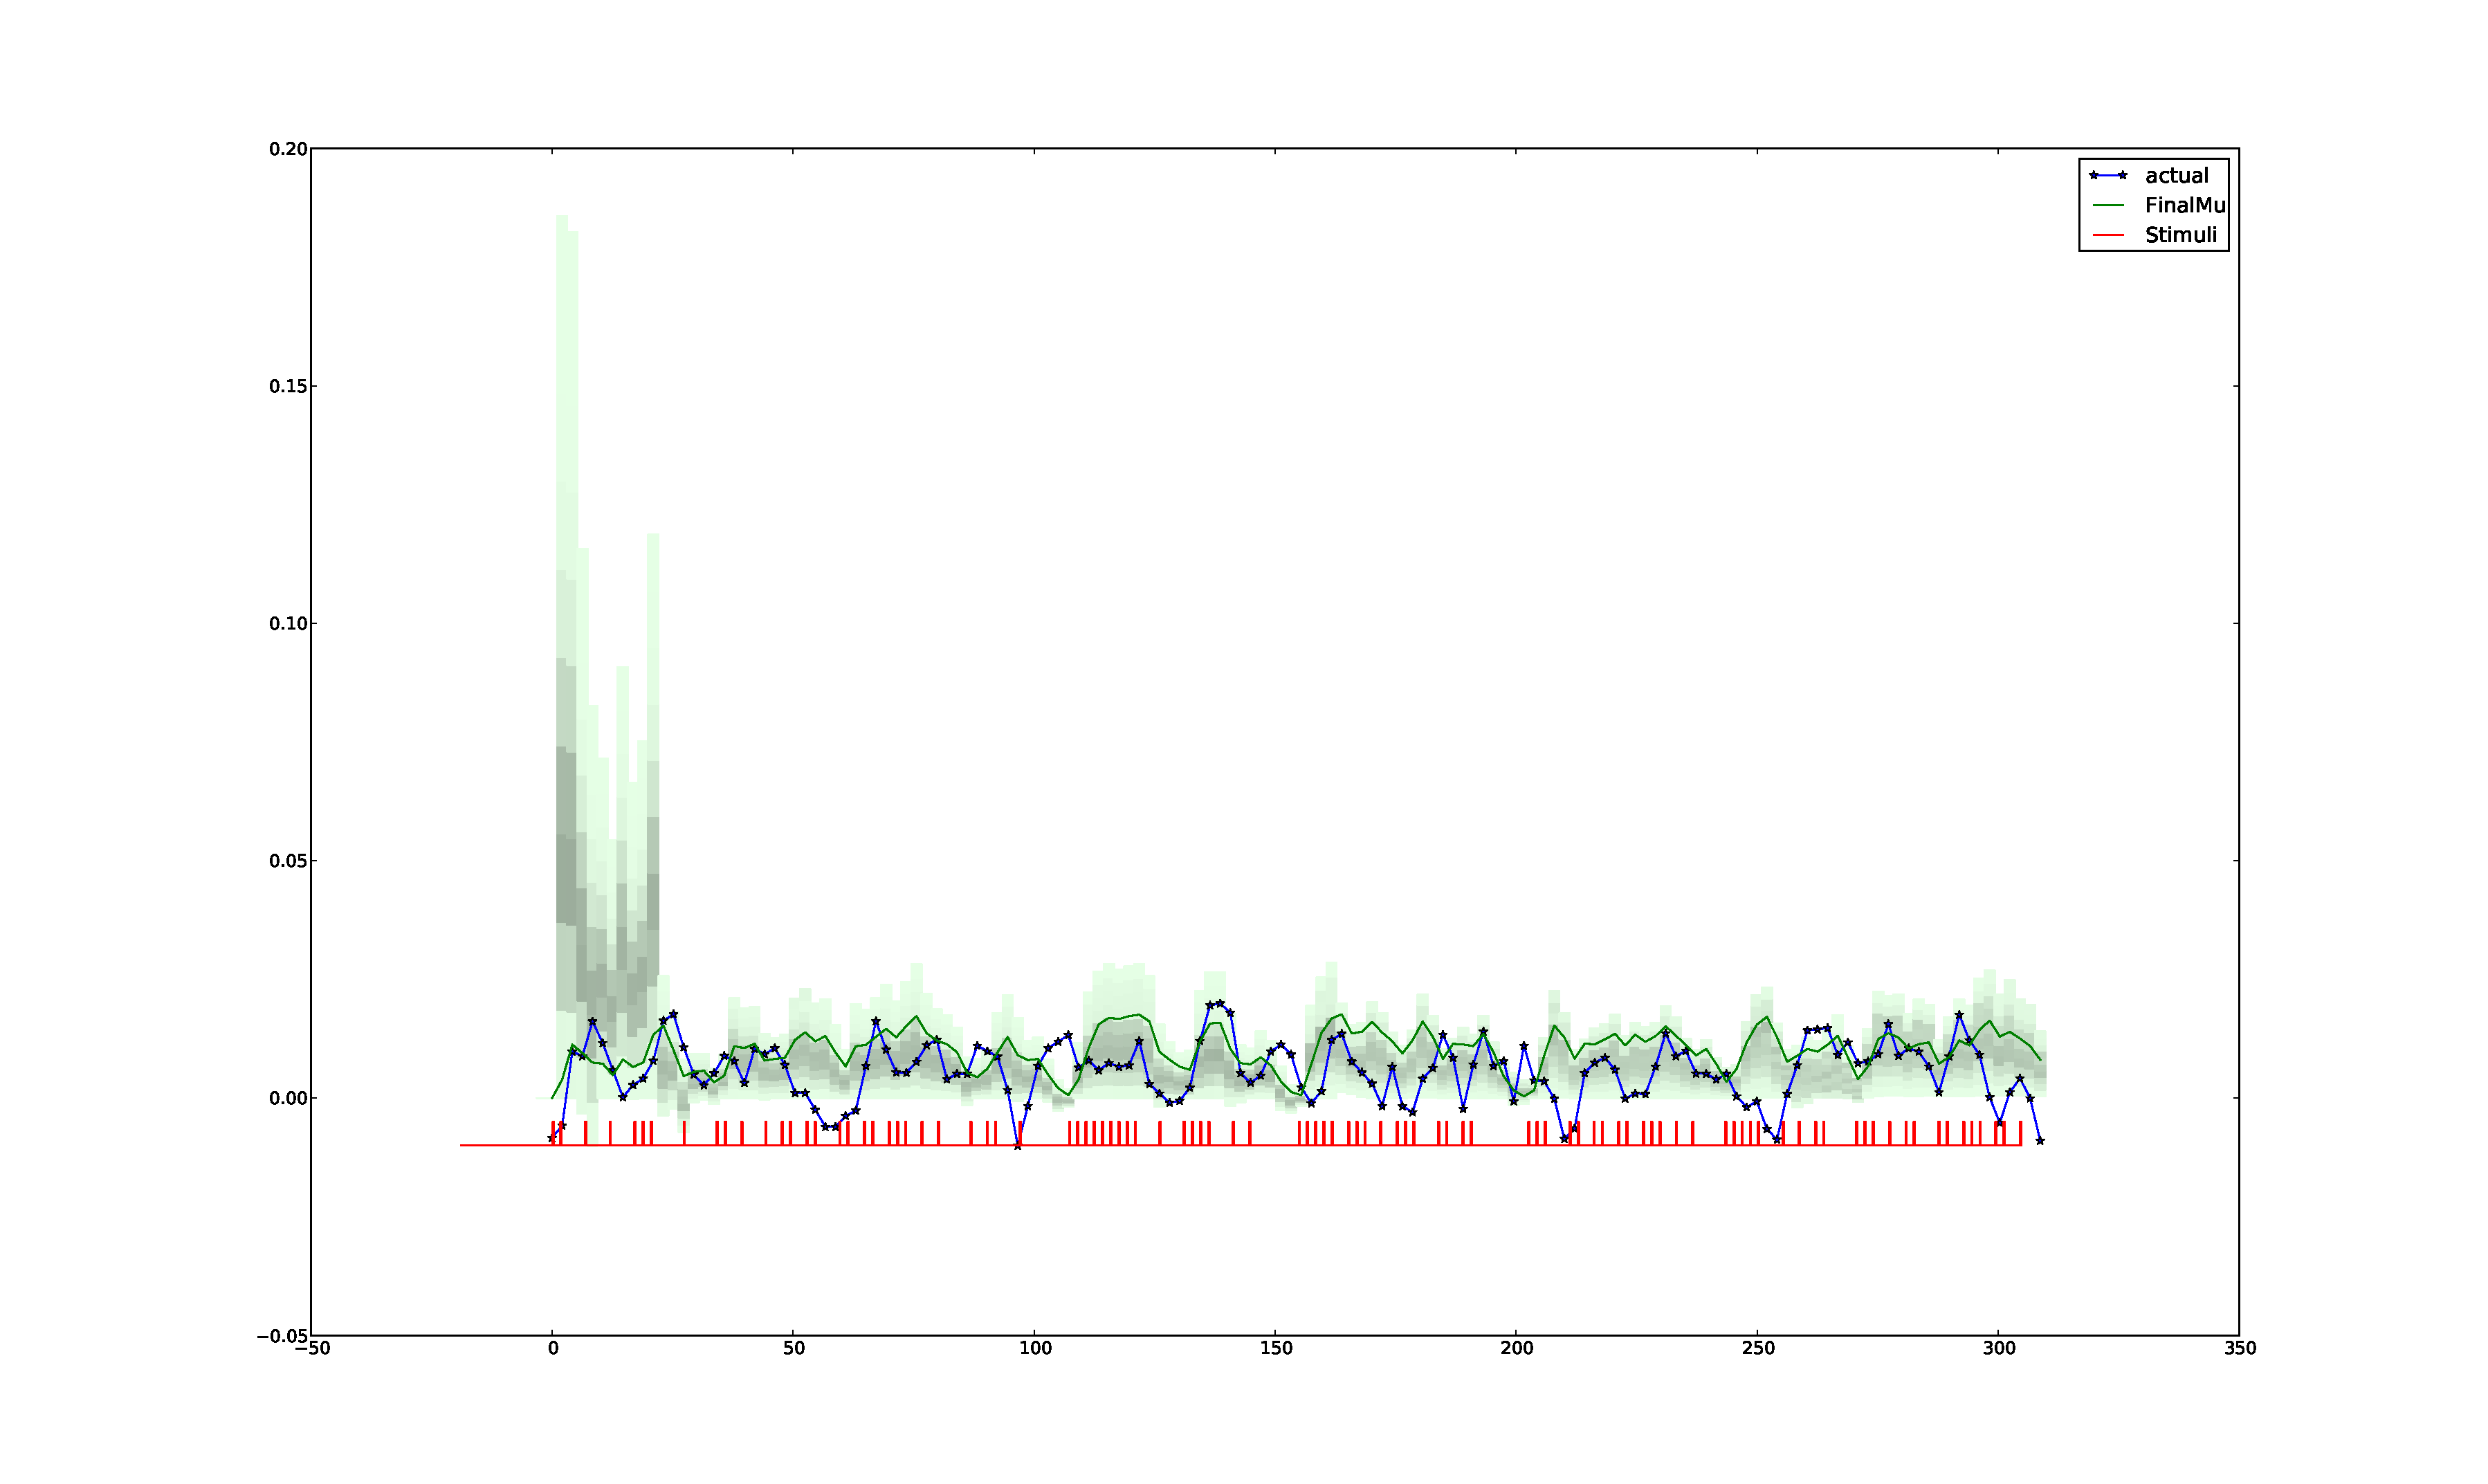
\includegraphics{images/goodfit_param1}}
\caption{The same priors gave rise to both fits. Params: ($\tau_0 \alpha E_0 V_0 \tau_f \tau_s \epsilon$)
for the good fit: $(1.40 .32 0.34 0.04  0.96 2.76)$, and for the poor fit:
$(2.28 0.32 0.33 0.017 0.67 2.88 1.36)$.}
\end{figure}

For this reason, I actually lowered the standard deviattions of the time
constants to prevent over-smoothing. This resulted in the more consistent, but
slightly worse results seen in \autoref{fig:param2_var}

\begin{figure}
\label{fig:param2_var}
\subfigure[]{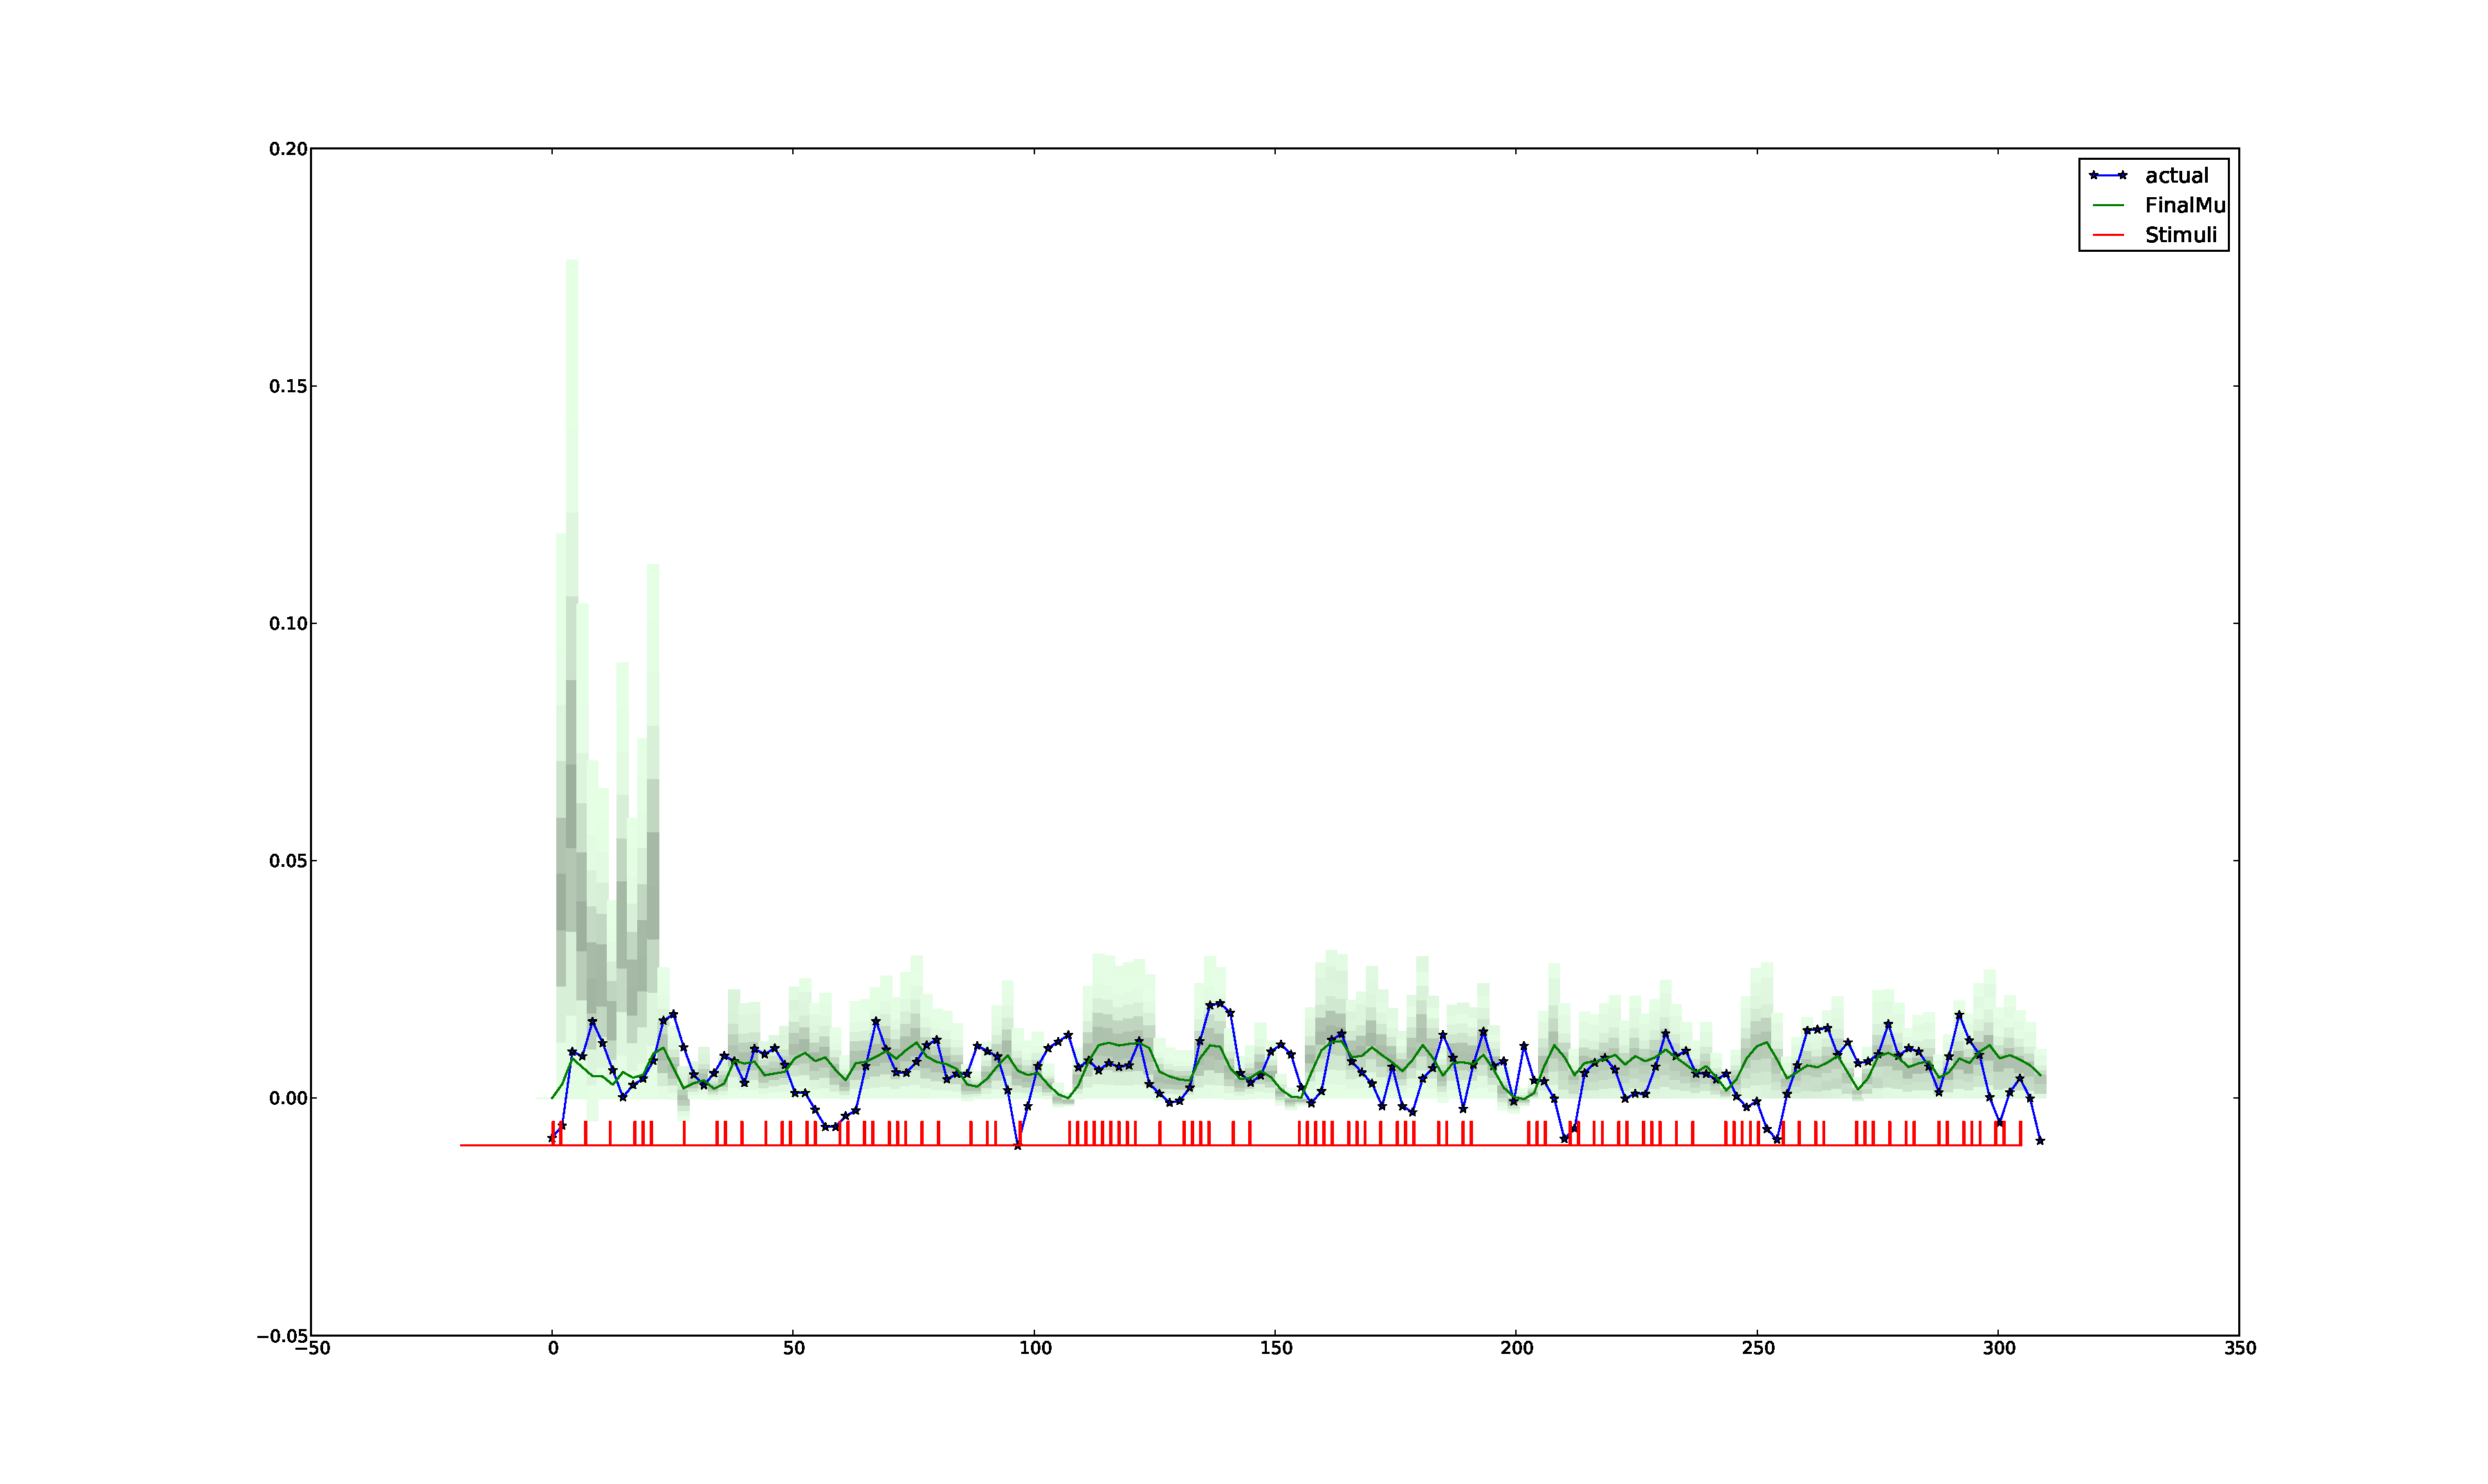
\includegraphics{images/param2a}}
\subfigure[]{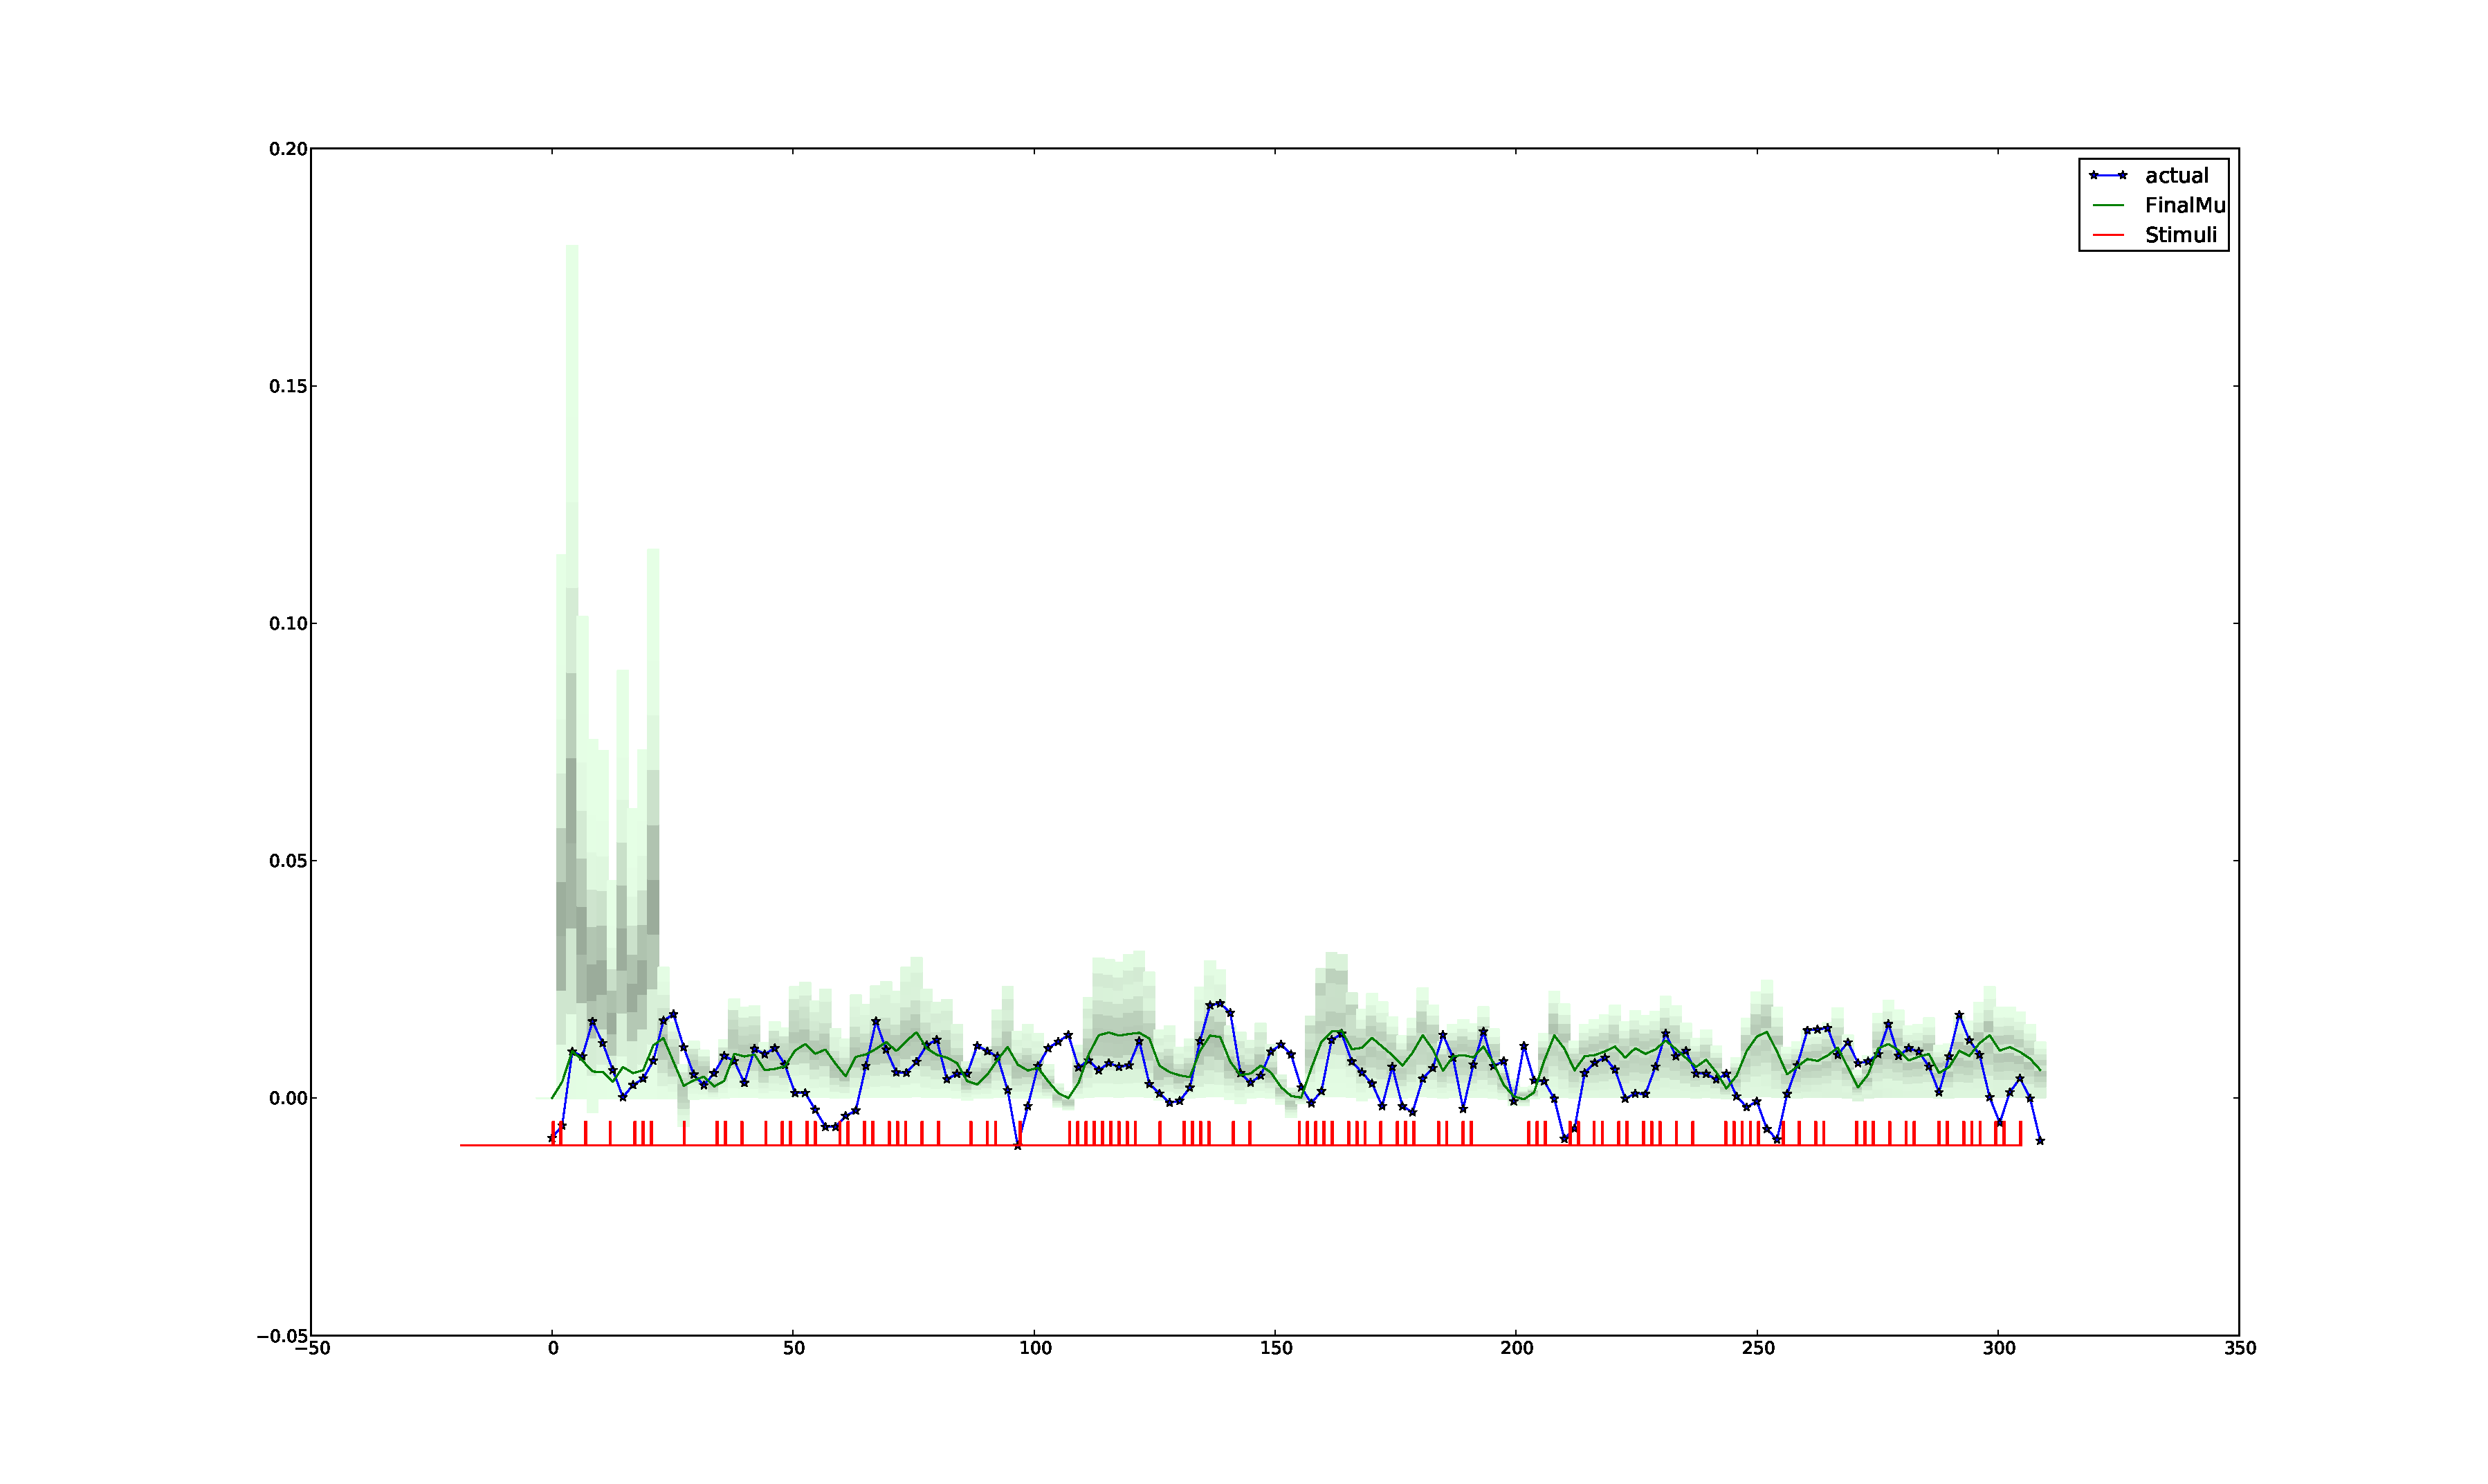
\includegraphics{images/param2b}}
\caption{A poor fit, using the same parameters as }
\end{figure}

\section{Particle Collapse Recovery}
This heuristic was initially intended to deal with cases where the particle
filter prematurely converged; and to reverse this effect. In reality, however
it did not perform well, and so it was not used in full-brain analysis. Ultimately
it did not prevent collapse of the distribution, and it often caused dramatic
increased in the variance of parameter estimates. It also pronged the analysis
time of inactive time series. Essentially the effect was exactly opposite of what
one would hope.


\section{Weighting Function Comparison}
\label{sec:Results Weights}

\section{Single Time-Series Simulation}

Graphs: 

For simulated data, single timeseries:

For \{delta, DC/Spline\}, \{exponential, gaussian, cauchy\}, \{biased, unbiased initial\},
\{100, 500, 1000\} particles
\begin{enumerate}
\item Ground truth vs. Estimated signal during particle filter run
\item Ground truth vs. Estimated signal with final parameter set
\item True Parameters vs. Final Parameter Sets
\item Variance of final parameters when faced with same ground truth, different noise
\item MSE of (a new timeseries based on X(t) vs. ground truth) for all t
\item Estimator Variance based on different noise runs
\item Final Particle Distribution
\end{enumerate}

For Simulated Data, Full Volume:

%note to self, epsilon should probably be uniform between 0 and something
\section{Simulated Volume}

\chapter{Real Data}
\begin{figure}
\label{fig:hm_canon_spm}
\subfigure[]{\label{fig:hm_spm} 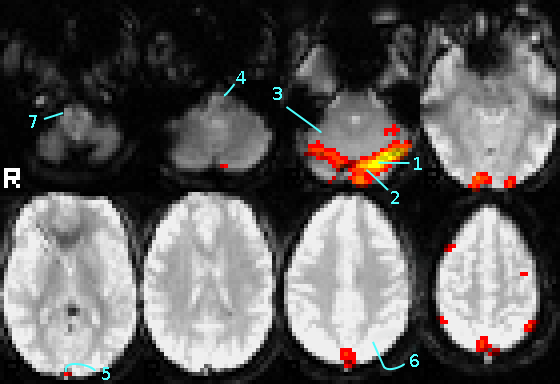
\includegraphics[scale=.66]{images/spm_hm}}
\subfigure[]{\label{fig:hm_canon_spm_x} 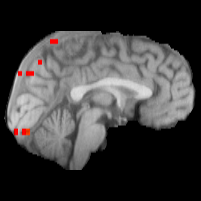
\includegraphics[scale=.85]{images/spm_hm_x}}
\subfigure[]{\label{fig:hm_canon_spm_y} 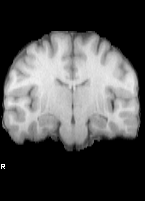
\includegraphics[scale=.85]{images/spm_hm_y}}
\subfigure[]{\label{fig:hm_canon_spm_z} 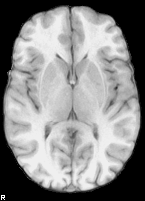
\includegraphics[scale=.85]{images/spm_hm_z}}
\subfigure{\label{fig:scale_spm} 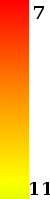
\includegraphics[scale=.3]{images/scale1}}
\caption{Sagittal, coronal and axial slices of SPM results (\autoref{fig:hm_canon_spm_x} \autoref{fig:hm_canon_spm_y} 
         \autoref{fig:hm_canon_spm_x}), as well as a series of axial slices, \autoref{fig:hm_spm}. Units
         of activation are in Student's T-scores. Higher indicates higher assurance that the signal cannot
         have occurred through noise alone.}
\end{figure}

\begin{figure}
\label{fig:hm_canon_pfilter}
\subfigure[]{\label{fig:hm_pfilter} 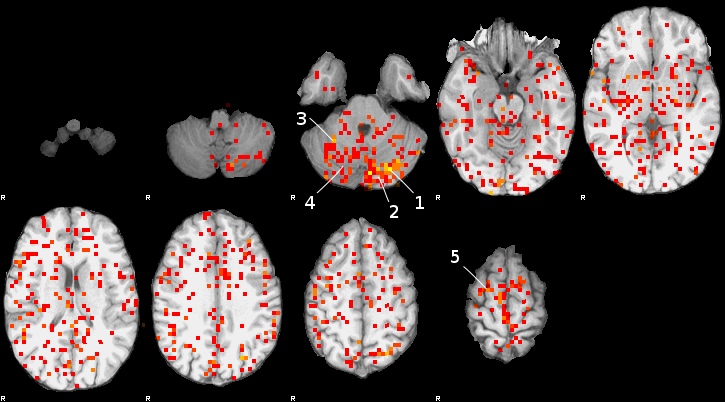
\includegraphics[scale=.66]{images/pfilter_hm}}
\subfigure[]{\label{fig:hm_canon_pfilter_x} 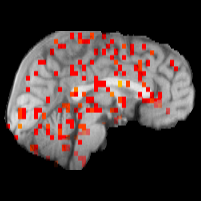
\includegraphics[scale=.85]{images/pfilter_hm_x}}
\subfigure[]{\label{fig:hm_canon_pfilter_y} 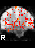
\includegraphics[scale=.85]{images/pfilter_hm_y}}
\subfigure[]{\label{fig:hm_canon_pfilter_z} 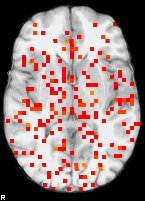
\includegraphics[scale=.85]{images/pfilter_hm_z}}
\subfigure{\label{fig:scale_pfilter} 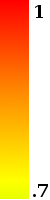
\includegraphics[scale=.3]{images/scale2}}
\caption{Sagittal, coronal and axial slices of SPM results (\autoref{fig:hm_canon_pfilter_x} \autoref{fig:hm_canon_pfilter_y} 
         \autoref{fig:hm_canon_pfilter_x}), as well as a series of axial slices, \autoref{fig:hm_pfilter}. 
         Units of match is normalized $\sqrt{MSE}$. The lowest (best) levels were $.7$,
         whereas the worst levels could go higher than 100 (not shown).}
\end{figure}

\begin{figure}
\label{fig:hm_canon_pfilter85}
\subfigure[]{\label{fig:hm_pfilter85} 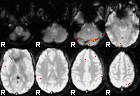
\includegraphics[scale=.66]{images/pfilter85_hm}}
\subfigure[]{\label{fig:hm_canon_pfilter85_x} 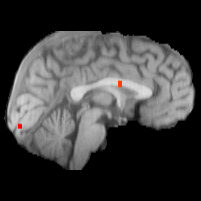
\includegraphics[scale=.85]{images/pfilter_hm85_x}}
\subfigure[]{\label{fig:hm_canon_pfilter85_y} 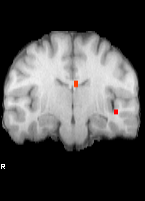
\includegraphics[scale=.85]{images/pfilter_hm85_y}}
\subfigure[]{\label{fig:hm_canon_pfilter85_z} 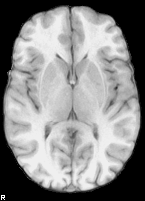
\includegraphics[scale=.85]{images/pfilter_hm85_z}}
\subfigure{\label{fig:scale_pfilter85} 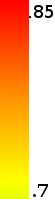
\includegraphics[scale=.3]{images/scale3}}
\caption{Sagittal, coronal and axial slices of SPM results (\autoref{fig:hm_canon_pfilter_x} \autoref{fig:hm_canon_pfilter_y} 
         \autoref{fig:hm_canon_pfilter_x}), as well as a series of axial slices, \autoref{fig:hm_pfilter}. 
         Units of match is normalized $\sqrt{MSE}$. The lowest (best) levels were $.7$,
         whereas the worst levels could go higher than 100 (not shown).}
\end{figure}

\begin{figure}
\label{fig:comp1}
\subfigure[Particle Filter]{\label{fig:comp1pfilter} \includegraphics[trim=5cm 1cm 4cm 1cm,width=15cm]{images/1_pfilter_37_14_7}}\\
\subfigure[SPM]{\label{fig:comp1spm} \includegraphics[trim=5cm 1cm 4cm 1cm,width=15cm]{images/1_spm_37_14_7}}
\caption{}
\end{figure}

\begin{figure}
\label{fig:comp2}
\subfigure[Particle Filter]{\label{fig:comp2pfilter} \includegraphics[trim=5cm 1cm 4cm 1cm,width=15cm]{images/2_pfilter_34_12_7}}\\
\subfigure[SPM]{\label{fig:comp2spm} \includegraphics[trim=5cm 1cm 4cm 1cm,width=15cm]{images/2_spm_34_12_7}}
\caption{}
\end{figure}

\begin{figure}
\label{fig:comp3}
\subfigure[Particle Filter]{\label{fig:comp3pfilter} \includegraphics[trim=5cm 1cm 4cm 1cm,width=15cm]{images/3_pfilter_23_21_7}}\\
\subfigure[SPM]{\label{fig:comp3spm} \includegraphics[trim=5cm 1cm 4cm 1cm,width=15cm]{images/3_spm_23_21_7}}
\caption{}
\end{figure}

\begin{figure}
\label{fig:comp4}
\subfigure[Particle Filter]{\label{fig:comp4pfilter} \includegraphics[trim=5cm 1cm 4cm 1cm,width=15cm]{images/4_pfilter_26_15_7}}\\
\subfigure[SPM]{\label{fig:comp4spm} \includegraphics[trim=5cm 1cm 4cm 1cm,width=15cm]{images/4_spm_26_15_7}}
\caption{}
\end{figure}

\begin{figure}
\label{fig:comp5}
\subfigure[Particle Filter]{\label{fig:comp5pfilter} \includegraphics[trim=5cm 1cm 4cm 1cm,width=15cm]{images/5_pfilter_25_34_25}}\\
\subfigure[SPM]{\label{fig:comp5spm} \includegraphics[trim=5cm 1cm 4cm 1cm,width=15cm]{images/5_spm_25_34_25}}
\caption{}
\end{figure}

image comparing epsilon-map with GLM activation map

